\chapter{Motohashi's formula for the fourth moment}\label{c5}

\section{Introduction and Statement fo results}\label{c5:sec5.1}

IN THIS CHAPTER\pageoriginale we shall study in detail $Y$. Motohashi's recent important work on the critical line. Instead of working directly with
 $$
 I_2 (T) = \int\limits^T_0 \left|\zeta \left(\frac{1}{2} + it \right)\right|^4 dt
 $$
 we shall deal with
 \begin{equation}
 \int\limits^\infty_{-\infty} \left|\zeta\left(\frac{1}{2} + iT + it \right) \right|^4 e^{-(t/\Delta)^2} dt \;\; \left(0 < \Delta \leq \frac{T}{\log T} \right),
 \label{c5:eq5.1}
 \end{equation}
 and then use later averaging techniques to obtain information about $I_2(T)$ itself, or about $E_2(T)$. The last function was defined in Chapter \ref{c4} as 
 \begin{equation}
 E_2 (T) = \int\limits^T_0 \left| \zeta\left( \frac{1}{2} + it\right)\right|^4 dt - TP_4 (\log T),\label{c5:eq5.2}
 \end{equation}
 where $P_4(y)$ is a suitable polynomial in $y$ of degree four with
 the leading coefficient equal to $1/(2\pi^2)$. The basic idea is to
 consider the following function of four complex variables $u,v,w,z$,
 namely 
{\fontsize{10pt}{12pt}\selectfont
 \begin{equation}
 I(u, v,w,z; \Delta) : = \frac{1}{\Delta \sqrt{\pi}} \int\limits^\infty_{-\infty} \zeta (u+ it) \zeta (v-it) \zeta (w+ it) \zeta (z - it) e^{-(t/\Delta)^2} dt.\label{c5:eq5.3}
 \end{equation}}
 For $\re u$, $\re v$, $\re w$, $\re z >1$ we have by absolute convergence
 \begin{align*}
& I (u,v,w,z;\Delta )\\
& = \frac{1}{\Delta \sqrt{\pi}} \sum\limits^\infty_{k=1}
   \sum\limits^\infty_{\ell=1} \sum\limits^\infty_{m=1}
   \sum\limits^\infty_{n=1} k^{-u} \ell^{-v} m^{-w} n^{-z}
   \int\limits^\infty_{-\infty} \exp \left(it \;\log \frac{\ell n}{km}
   - t^2 \Delta^{-2}\right) dt\\ 
& = \sum\limits^\infty_{k, \ell, m, n=1} k^{-u} \ell^{-v} m^{-w} n^{-z}\exp \left(-\left(\frac{\Delta}{2} \log \frac{\ell n}{km} \right)^2 \right), 
 \end{align*}
 since 
 $$
 \int\limits^\infty_{-\infty} e^{Ax -Bx^2} dx = \sqrt{\frac{\pi}{B}}
 e^{A^2/(4B)} \quad (\re B > 0). 
 $$\pageoriginale
 Following the initial step in Atkinson's treatment of $E(T)$ (see (\ref{c2:eq2.7}) and (\ref{c2:eq2.8})) one writes then
{\fontsize{10pt}{12pt}\selectfont 
\begin{align}
 I(u,v,w,z;\Delta) & = \left\{ \sum\limits_{km = \ell n} +
 \sum\limits_{km< \ell n} + \sum\limits_{km > \ell n} \right\} k^{-u}
 \ell^{-v} m^{-w}  n^{-z}\times
\exp \left(- \left(\frac{\Delta}{2} \log
 \frac{\ell n}{ km} \right)^2 \right)\notag\\ 
 & = I_1 (u,v,w,z; \Delta) + I_2 (u,v,w,z;\Delta) + I_3 (u,v,w, z;\Delta),\label{c5:eq5.4}
 \end{align}}
 say. In $I_1$ we have $n=km/\ell$, hence
 \begin{align*}
& I_1(u,v,w,z;\Delta) = \sum\limits_{k,m,\ell, n \geq 1; km=\ell n} \ell^{z-v_m u-w} (km)^{-u-z}\\
& = \sum\limits^\infty_{r=1} \left(\sum\limits_{\ell n = r} \ell^{z-v} \right) \left(\sum\limits_{km=r} m^{u-w} \right) r^{-u-z} = \sum\limits^{\infty}_{r=1} \sigma_{z-v} (r) \sigma_{u-w} (r) r^{-u-z}.
 \end{align*}

 To evaluate the last series we recall a classical identity of
 S. Ramanujan. This is  
 \begin{equation}
 \sum\limits^\infty_{n=1} \sigma_a (n) \sigma_b (n) n^{-s} = \frac{\zeta(s) \zeta(s-a) \zeta (s-b) \zeta(s-a-b)}{\zeta(2s-a-b)}\label{c5:eq5.5}
 \end{equation}

 It is valid for $\re s > \max (1, \re  a+ 1, \re b + 1, \re a + \re b + 1)$ and can be proved by expanding both sides into an Euler product, since $\sigma_z(n)$ is a multiplicative function of $n$ for any $z$. Setting $s = u +z$, $a = z - v$, $b = u - w$ we obtain
 \begin{equation}
 I_1(u,v,w,z;\Delta) = \frac{\zeta (u+v) \zeta (u+z) \zeta (v+w) \zeta
   (w+z)}{\zeta(u+v+w+z)}, \label{c5:eq5.6} 
\end{equation}
thereby providing analytic continuation of $I_1$ as a meromorphic
function of $u,v,w,z$ over $\mathbb{C}^4$. By symmetry 
 \begin{equation}
 I_3 (u,v,w,z;\Delta) = I_2 (v,u,z,w;\Delta),\label{c5:eq5.7} 
 \end{equation}
 and the main task is to prove that $I_2 (u,v,w,z;\Delta)$ also exists
 as a meromorphic function of $u,v,w,z$ on $\mathbb{C}^4$. We are
 interested in (\ref{c5:eq5.3}) for $u = \frac{1}{2} + i T$, $v =
 \frac{1}{2} - iT $, $w = \frac{1}{2} + iT$, $z = \frac{1}{2} - iT$,
 that is, in the\pageoriginale analytic continuation of the function
 defined initially by (\ref{c5:eq5.3}). Henceforth we shall assume
 that $I(u,v,w,z;\Delta)$ stands for the meromorphic function of
 $u,v,w,z$ on $\mathbb{C}^4$ defined initially by (\ref{c5:eq5.3}). 

 It is not difficult to show that
 \begin{align}
 & I \left(\frac{1}{2} + i T, \frac{1}{2} - iT, \frac{1}{2} +iT, \frac{1}{2} - i T;\Delta \right) = \label{c5:eq5.8}\\
 & \qquad \frac{1}{\Delta\sqrt{x}} \int\limits^\infty_{-\infty} \left|\zeta \left(\frac{1}{2} + i T+ it \right)\right|^4 e^{-(t/\Delta)^2} dt + \frac{\sqrt{x}}{\Delta} \re\notag\\
& \qquad  \left\{ \left(\gamma - \log 2 \pi + \Delta^{-2} \left(\frac{1}{2} + i T \right)  \right) \exp \left( \left(\frac{\frac{1}{2}  + iT}{\Delta} \right)^2 \right) \right\},\notag 
 \end{align}
  and the last expression is $O \left(\exp \left(-\dfrac{1}{2} \log^2 T \right) \right)$ for $0 < \Delta \leq \dfrac{T}{\log T}$.  The analytic continuation of $I_2 (u,v,w,z;\Delta)$ is carried out in several steps, to a region in which it admits an expression in terms of sums of Kloosterman sums
 \begin{equation}
 S(m,n;c) = \sum\limits_{1 \leq d \leq c , (d,c) = 1, d d' \equiv 1 (\mod c)} e\left(\frac{md+nd'}{c} \right),\label{c5:eq5.9}
 \end{equation}
 where $e(x) = e^{2\pi ix}$. This analytic continuation will be given
 in detail in Section \ref{c5:sec5.2}. It turns out that one can
 successfully apply the powerful machinery of Kuznetsov's trace
 formula and the spectral theory of automorphic forms to the resulting
 expression for analytic continuation. This will be discussed in
 Section \ref{c5:sec5.3}, while in Section \ref{c5:sec5.4} we shall
 obtain an explicit formula for (\ref{c5:eq5.1}) which requires a
 considerable amount of technical work. This is Motohashi's main
 result, which we state here as 

\setcounter{thm}{0}
 \begin{thm}\label{c5:thm5.1}
 If $0 < \Delta \leq I / \log  T$, then 
 \begin{align}
&  \frac{1}{\Delta \sqrt{\pi}} \int\limits^\infty_{-\infty}
   \left|\zeta \left(\frac{1}{2}+ iT + it\right) \right|^4 e^{-
     (t/\Delta)^2} dt \label{c5:eq5.10} \\ 
 & \qquad = F_0(T,\Delta) + \frac{1}{\pi} \int\limits^\infty_{-\infty}
   \frac{\left|\zeta \left(\frac{1}{2} + i \xi
     \right)\right|^6}{\left|\zeta(1+ 2i\xi)\right|^2} \theta (\xi; T,
   \Delta) d\xi\notag\\ 
&  \qquad = \sum\limits^\infty_{j=1} \alpha_j H^3_j \left(\frac{1}{2}
   \right) \theta (x_j; T,\Delta)\notag\\
&\qquad + \sum\limits^\infty_{k=6} \sum\limits^{d_{2k}}_{j=1} \alpha_{j,2k} 
H^3_{j,2k} \left(\frac{1}{2} \right) \Lambda (k; T, \Delta) + O\left(T^{-1}
\log^2 T\right), \notag
 \end{align}
 where\pageoriginale $\alpha_j,a_{j,2k}$ and the functions $H_j$, $H_{j,2k}$ are defined in Section \ref{c5:sec5.3}; $F_0, \theta, \Lambda$ by (\ref{c5:eq5.112}) and (\ref{c5:eq5.110}). The $0$-constant in (\ref{c5:eq5.10}) is absolute.
 \end{thm}

 One can evaluate explicitly $F_0(T,\Delta)$ as follows. From Stirling's formula one has
 $$
 \Gamma' (s)  = \Gamma(s) \left(\log s -\frac{1}{2s} + a_2 s^{-2} + \ldots + a_rs^{-r} + F_r(s)\right)
 $$
 with $F_r(s) \ll_r |s|^{-r-1}$. Hence by successive differentiation
 $$
 \frac{\Gamma^{(k)}(s)}{\Gamma(s)} = \sum\limits^k_{j=0} b_{j,k} (s) \log^j s + c_{-1, k} s^{-1} + \ldots  + c_{-r, k} s^{-r} + 0 \left(_r |s|^{-r-1}\right)
 $$
 for any fixed integers $k \geq 1$, $r \geq 0$, where each $b_{j,k} (s)$ ($\sim b_{j,k}$ for a suitable constant $b_{j,k}$) has an expansion in nonpositive powers of $s$. From (\ref{c5:eq5.112}) it is seen that in evaluating $F_0(T,\Delta)$ we encounter sums which involve, for $0 \leq r \leq 4$,
 \begin{align*}
 & \re \left\{\frac{1}{\Delta \sqrt{\pi}} \int\limits^\infty_{-\infty}
   \log^r \left(\frac{1}{2} + iT + it \right) e^{-(t/\Delta)^2}
   dt\right\}\\ 
 & \qquad = \pi^{-\frac{1}{2}} \re \left\{
   \int\limits^\infty_{-\infty} \log^r \left(\frac{1}{2} +iT +
   iu\Delta \right) e^{-u^2} du \right\}\\ 
 & \qquad =  \pi^{-\frac{1}{2}} \re \left\{  \int\limits^{\log
     T}_{-\log T} \log^r \left(\frac{1}{2} + iT + i u\Delta \right)
   e^{-u^2} du\right\} + O_A(T^{-A}) 
 \end{align*}
 for any fixed $A > 0$. For $|u| \leq \log T$ one has the power series expansion
 \begin{align*}
 \log^r \left(\frac{1}{2} + iT + i u \Delta \right) & = (\log iT)^r +
 \sum\limits^r_{k=1} \binom{r}{k} (\log iT)^{r-k} \\ 
& \qquad \left(\frac{u\Delta}{T} + \frac{1}{2iT} - \frac{1}{2}
 \left(\frac{u\Delta}{T} + \frac{1}{2iT} \right)^2 + \ldots
 \right)^k. 
 \end{align*}

Thus in the range $0 < \Delta \leq T \exp (-\sqrt{\log T}) $ we have 
\begin{equation}
 F_0(T,\Delta) = Q_4 (\log T) + O \left(\exp \left(-\frac{1}{2} \sqrt{\log T } \right) \right), \label{c5:eq5.11}
 \end{equation}
 where\pageoriginale $Q_4(y)$ is a polynomial of degree four whose
 coefficients may be explicitly evaluated. 

 A remarkable feature of Theorem \ref{c5:thm5.1} is that the error
 term appearing in it is quite small. This makes it a powerful
 instrument in the study of $\zeta(s)$  in general, with greater, with
 greater potential and applicability than the formulas for the fourth
 moment of Heath-Brown and Zavorotnyi that were discussed in Chapter
 \ref{c4}. By more careful analysis, involving the evaluation of
 certain exponential integrals by the saddle-point method, it is
 possible to transform the right-hand side of (\ref{c5:eq5.10}) into a
 more explicit form, at the cost of a poorer error term and a shorter
 range for $\Delta$. This will be effected in Section \ref{c5:sec5.5},
 and the result is the following theorem (all the relevant notation is
 defined in Section \ref{c5:sec5.3}): 

 \begin{thm}\label{c5:thm5.2}
 If $T^{\frac{1}{2}} \log^{-A} T \leq \Delta \leq T \exp (-\sqrt{\log T})$ where $A>0$ is arbitrary but fixed, then there exists $C = C(A) >0$ such that uniformly in $\Delta$
 \begin{align}
& \frac{1}{\Delta \sqrt{\pi}} \int\limits^\infty_{-\infty} \left|\zeta \left(\frac{1}{2} + i T + it \right)\right|^4 e^{-(t/\Delta)^2} dt\label{c5:eq5.12}\\
& = \pi 2^{-\frac{1}{2}} T^{-\frac{1}{2}}  \sum\limits^\infty_{j=1}
   \alpha_j x^{-\frac{1}{2}}_j H^3_j \left(\frac{1}{2} \right) \sin
   \left(x_j \log \frac{x_j}{4eT} \right) e^{-(\Delta x_j/ 2T)^2} + O
   (\log^CT).\notag 
 \end{align}
 \end{thm}

 By (\ref{c5:eq5.11}) we have $F_0(T,\Delta) \gg \log^4T$, so that $C \geq 4$ in (\ref{c5:eq5.12}). It is also useful to have an integrated version of (\ref{c5:eq5.12}).

 \begin{thm}\label{c5:thm5.3}
 If $V^{\frac{1}{2}} \log {}^{-A} V \leq \Delta \leq V \exp (-\sqrt{\log V})$, where $A>0$ is arbitrary but fixed, then there exists $C = C(A) > 0$ such that uniformly in $\Delta$
{\fontsize{10pt}{12pt}\selectfont
 \begin{align}
&  \frac{1}{\Delta \sqrt{\pi}} \int\limits^V_0
   \int\limits^\infty_{-\infty} \left|\zeta \left(\frac{1}{2} + iT +
   it \right) \right|^4 e^{-(t/\Delta)^2} dt \; dT
    \label{c5:eq5.13}\\  
& \quad = VP_4 (\log V)  + \pi \left(\frac{V}{2} \right)^{\frac{1}{2}} 
 \sum\limits^\infty_{j=1} \alpha_j H^3_j \left(\frac{1}{2} \right)
 x^{-3/2}_j \cos \left(x_j \log \frac{x_j}{4eV} \right) e^{-(\Delta x_j
   / 2V)^2}\notag\\
&\quad + O\left(V^{\frac{1}{2}} \log^C V\right) + O(\Delta \log^5 V),\notag 
 \end{align}}
 where $P_4(y)$\pageoriginale is a suitable polynomial of degree four
 in $y$. Moreover, if $V^{\frac{1}{2}} \log^{-A} V \leq \Delta \leq
 V^{\frac{3}{4}}$, then  
 \begin{align}
&  \frac{1}{\Delta \sqrt{\pi}} \int\limits^V_0
   \int\limits^\infty_{-\infty} \left|\zeta \left(\frac{1}{2} + iT +
   it \right)\right|^4 e^{-(t/\Delta)^2} dt \; dT = VP_4 (\log V)\notag \\ 
& \qquad  +\pi \left(\frac{V}{2} \right)^{\frac{1}{2}}
   \sum\limits^\infty_{j=1} \alpha_j H^3_j \left(\frac{1}{2} \right)
   c_j \cos \left(x_j \log \frac{x_j}{4eV} \right)\notag\\ 
& \qquad e^{-(\Delta x_j / 2 V)^2} + O (V^{\frac{1}{2}}) + O (\Delta \log^5 V),\label{c5:eq5.14}
 \end{align}
 where, as $j \to \infty$,
 $$
 c_j = (1+ o(1)) x^{-3/2}_j. 
 $$
 \end{thm}

 In fact, it is not difficult to see that $P_4$ is the same polynomial which appears in the definition (\ref{c5:eq5.2}) of $E_2(T)$ (see also (\ref{c4:eq4.3}) and (\ref{c4:eq4.4})), and it is possible to deduce an upper bound for $E_2(T)$ from Theorem \ref{c5:thm5.3}. This is 

 \begin{thm}\label{c5:thm5.4}
 There is an absolute constant $C>0$ such that 
 \begin{equation}
 E_2(T) \ll T^{2/3} \log^C T. \label{c5:eq5.15}
 \end{equation}
 \end{thm}

 This upper bound is a slightly sharper form of the result
 (\ref{c4:eq4.6}) of N. Zavorotnyi. We can also obtain integral
 averages of $E_2(T)$ which correspond to Theorem \ref{c3:thm3.1} and
 Theorem \ref{c3:thm3.7} for $E_1(T) = E(T)$. This is 

\begin{thm}\label{c5:thm5.5}
We have
\begin{equation}
\int\limits^T_0 E_2(t) dt \ll T^{3/2}\label{c5:eq5.16}
\end{equation}
and
\begin{equation}
\int\limits^T_0 E_2(t) \left|\zeta \left(\frac{1}{2} + it
\right)\right|^4 dt \ll T^{3/2} \log^4 T.\label{c5:eq5.17} 
\end{equation}

We also have a mean square result on $E_2(T)$, contained in 
\end{thm}

\begin{thm}\label{c5:thm5.6}
There is a suitable constant $C>0$ such that uniformly for $T^{2/3}
\ll H \leq T$ 
\begin{equation}
\int\limits^{T+H}_T E^2_2(t) dt \ll T^{3/2} H^{3/4} \log^C
T.\label{c5:eq5.18} 
\end{equation}\pageoriginale
\end{thm}

The previous theorems dealt with upper bound results. However, we can also obtain an omega-result for $E_2(T)$. The result, which is one of the most important applications of the explicit formula for the fourth moment, is 

\begin{thm}\label{c5:thm5.7}
\begin{equation}
E_2(T) = \Omega (T^{\frac{1}{2}}). \label{c5:eq5.19}
\end{equation}
\end{thm}

In the proof of Theorem \ref{c5:thm5.7}, given in Section
\ref{c5:sec5.7}, we shall make  use of a non-vanishing type of result
for automorphic $L$-functions, proved recently by
Y. Motohashi. However, if one could prove a certain linear
independence over the integers of spectral values, then we shall that
(\ref{c5:eq5.19}) may be replaced by the stronger 
$$
\limsup\limits_{T\to \infty} |E_2 (T)| T^{-\frac{1}{2}} = + \infty.
$$

Finally, we shall reprove an important result of $H$. Iwaniec on sums
of integrals of $|\zeta \left(\frac{1}{2} + it \right)|^4$ in short
intervals. In fact we improve on Iwaniec's result by obtaining
log-powers where we had $T^\epsilon$. This is  

\begin{thm}\label{c5:thm5.8}
Suppose $R < t_1 < t_2 < \ldots < t_R \leq 2T$ with $t_{r+1} - t_r > \Delta$ $(r = 1,2,\ldots, R-1 )$ and $T^{\frac{1}{2}} \leq \Delta \leq T$. Then there exist constants $C_1, C_2 >0$ such that 
$$
\sum\limits_{r\leq R} \int\limits^{t_r+\Delta}_{t_r} \left|\zeta \left(\frac{1}{2} + it \right)\right|^4 dt \ll R \Delta \log^{C_1} T + R^{\frac{1}{2}} T \Delta^{-\frac{1}{2}} \log^{C_2} T. 
$$
\end{thm}

We shall prove Theorems \ref{c5:thm5.4} - \ref{c5:thm5.6} and Theorem \ref{c5:thm5.8} in Section \ref{c5:sec5.1}. We remark that Theorem \ref{c5:thm5.8} yields
$$
\int\limits^T_0 \left|\zeta \left(\frac{1}{2} + it \right) \right|^{12} dt \ll T^2 \log^D T
$$\pageoriginale
as a corollary with an effectively computable $D >0$. The above estimate, with $D=17$, was proved first by D.R. Heath-Brown.

\section{Analytic Continuation}\label{c5:sec5.2}

As the first step we shall establish (\ref{c5:eq5.8}), which is important because the integral (\ref{c5:eq5.1}) appears on the right-hand side. In (\ref{c5:eq5.3}) we move the line of integration to $\mathscr{L}$, as follows:

\begin{figure}[H]
\centering
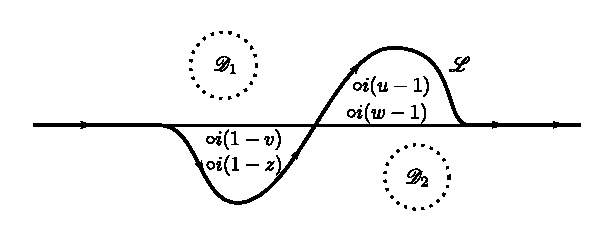
\includegraphics{figures/fig1.eps}
\end{figure}


Then we have, for $\re u$, $\re v$, $\re w$, $\re z >1$, by the residue theorem
\begin{align*}
& I (u,v,w,z;\Delta) = \frac{1}{\Delta \sqrt{\pi}}
  \int\limits_{\mathscr{L}} \zeta (u + it) \zeta(v - it) \zeta(w + it)
  \zeta(z - it) e^{-(t/\Delta)^2} dt \\ 
&\quad + \frac{2}{\Delta} \pi^{\frac{1}{2}} \left\{ \zeta (u+ v -1)
  \zeta(w-u+1) \zeta(u+z-1) \exp \left( \left(\frac{u-1}{\Delta}
  \right)^2\right) \right.\\ 
&\quad + \zeta(u+v-1) \zeta(v+w-1) \zeta(z-v+1) \exp
  \left(\left(\frac{v-1}{\Delta} \right)^2\right)\\ 
&\quad + \zeta(u-w+1) \zeta(v+w-1) \zeta(w+z-1) \exp
  \left(\left(\frac{w-1}{\Delta} \right)^2\right)\\ 
&\quad \left. + \zeta(u+z-1) \zeta (v-z+1) \zeta(w+z-1) \exp
  \left(\left(\frac{z-1}{\Delta} \right)^2 \right) \right\}. 
\end{align*}

Namely, there are simple poles of the integrand at the points $t =
(1-u)/i$, $(1-w)/i$, $(v-1)/i$, $(z-1)/i$ and e.g. 
$$
\lim\limits_{t \to (1-u)/i} \zeta(u+it) \left(t - \frac{1-u}{i} \right) = \frac{1}{i}, 
$$
hence the above relation follows. It obviously holds for those
$u,v,w,z$\pageoriginale such that $i(1-v)$, $i(1-z) \in
\mathscr{D}_1$, and $i(u-1)$, $i(w-1) \in \mathscr{D}_2$. Then
$\mathscr{L}$ can be replaced by the real axis, and we obtain for any
$T>0$ and $\re u$, $\re v$, $\re w$, $\re z <1$, 
\begin{align}
& I(u+ iT, v - iT, w + iT, z - i T; \Delta)\label{c5:eq5.20}\\
&\quad = \frac{1}{\Delta \sqrt{\pi}} \int\limits^\infty_{-\infty} \zeta(u+iT
+ it) \zeta(v-iT-it) \zeta (w+ iT + it)\notag\\ 
&\hspace{6cm}\zeta (z-iT - it) e^{-(t/\Delta)^2} dt\notag\\
&\quad + \frac{2\pi^{\frac{1}{2}}}{\Delta} \left\{ \zeta (u+v-1)
\zeta(w-u+1) \zeta(u+z-1) \exp \left( \left(\frac{u+iT
  -1}{\Delta}\right)^2 \right)\right.\notag\\ 
&\quad + \zeta (u+v-1) \zeta(v+w-1) \zeta(z-v+1) \exp \left(
\left(\frac{v-iT-1}{\Delta} \right)^2\right)\notag\\ 
&\quad + \zeta(u-w+1) \zeta(v+w-1) \zeta(w+z-1) \exp \left( \left(
\frac{w+iT-1}{\Delta}\right)^2\right)\notag\\ 
&\quad \left. + \zeta(u+z-1) \zeta(v-z+1) \zeta(w+z-1) \exp \left(\left(\frac{z-iT-1}{\Delta} \right)^2 \right) \right\}.\notag
\end{align}

When $(u,v,w,z)$ is in the neighbourhood of the point $
\left(\frac{1}{2}, \frac{1}{2}, \frac{1}{2}, \frac{1}{2} \right)$, the
points $u+v-1$, $w-u+1$ etc. appearing in curly braces in
(\ref{c5:eq5.20}) are close to 0 and 1. Using the power series
expansion of $\zeta(s)$ near these points and simplifying we obtain
(\ref{c5:eq5.8}) from (\ref{c5:eq5.20}). 

The next step is to seek analytic continuation of the functions $I_2$
and $I_3$, defined by  (\ref{c5:eq5.4}), in the case $u=\frac{1}{2} +
iT$, $v = \frac{1}{2} - iT$, $w = \frac{1}{2} + iT$, $z = \frac{1}{2}
- iT$. We can write, for $\re u$, $\re v$, $\re w$, $\re z >1$, 
{\fontsize{10pt}{12pt}\selectfont
\begin{align*}
& I_2 (u+iT, v - iT, w + iT, z- iT; \Delta)\\
& = \sum\limits^{\infty}_{m_1, m_2, n_1, n_2 =1; m_1 m_2 < n_1 n_2}
m_1^{-u-iT} m^{-w-iT}_2 n_1^{-v+iT} n_2^{-z+iT}
 \exp \left( -\left(\frac{\Delta}{2} \log \frac{n_1 n_2}{m_1 m_2}
\right)^2\right).   
\end{align*}}

We group together terms with $m_1m_2 = m$, set $n_1 n_2 = m+n$, so
that $m,n \geq 1$. Thus we obtain 
\begin{align*}
& I_2 (u+iT, v - iT, w + iT, z - iT; \Delta)\\
& \qquad = \sum\limits^\infty_{m,n=1} m^{-u} (m+n)^{-v} \left(\sum\limits_{m_2|m} m^{u-w}_2 \right) \left(\sum\limits_{n_2|(m+n)} n^{v-z}_2 \right) \\
& \qquad \qquad  \qquad  \left(1+\frac{n}{m} \right)^{iT} \exp \left(- \left(\frac{\Delta}{2} \log \left(1+ \frac{n}{m} \right) \right)^2 \right)\\
& \qquad = \sum\limits^\infty_{m,n=1} \sigma_{u-w} (m) \sigma_{v-z} (m+n) \left(1+\frac{n}{m} \right)^{-v+iT}\\
& \qquad \qquad \qquad   m^{-u-v} \exp \left(- \left(\frac{\Delta}{2} \log \left(1+ \frac{n}{m} \right) \right)^2 \right).
\end{align*}\pageoriginale

To transform further the last expression we set $p=s$, $q=w-s$ in the
beta-integral formula 
$$
\frac{\Gamma(p) \Gamma(q)}{\Gamma(p+q)} = \int\limits^\infty_0
\frac{x^{p-1}}{(1+x)^{p+q}} dx \quad (\re p, \re q > 0) 
$$
to obtain
$$
\frac{\Gamma (s) \Gamma (w-s)}{\Gamma(w)} = \int\limits^{\infty}_0
(1+x)^{-w} x^{s-1} dx. 
$$

This means that $F(s) = \Gamma (s) \Gamma (w-s) / \Gamma (w)$ (for $w$
fixed) is the Mellin transform of $f(x) = (1+x)^{-w}$. Hence by the
Mellin inversion formula 
\begin{equation}
\Gamma(w) (1+x)^{-w} = \frac{1}{2\pi i} \int\limits^{a+ i
  \infty}_{a-i\infty} \Gamma(s) \Gamma (w-s) x^{-s}
ds,\label{c5:eq5.21} 
\end{equation}
where $\re w > a > 0$, $x > 0$. We divide (\ref{c5:eq5.21}) by $\Gamma(w)$, replace $w$ by $w+ it$, multiply by $\exp (-(t/\Delta)^2)$ and integrate over $t$. Using the exponential integral as in the transformation of (\ref{c5:eq5.3}) we have
\begin{align}
& (1+x)^{-w} \exp \left(- \left(\frac{\Delta}{2} \log (1+x) \right)^2 \right)\label{c5:eq5.22}\\
& = \frac{1}{2\pi i} \; \frac{1}{\Delta \sqrt{\pi}}
  \int\limits^{\infty}_{-\infty}
  \frac{e^{-(t/\Delta)^2}}{\Gamma(w+it)}
  \int\limits^{a+i\infty}_{a-i\infty} \Gamma(s) \Gamma (w+it-s) x^{-s}
  ds \; dt\notag\\ 
& = \frac{1}{2\pi i} \int\limits^{a+i\infty}_{a-i\infty} M(s, w;
  \Delta) x^{-s} ds,\notag 
\end{align}
where the interchange of integration is justified by absolute
convergence, and where we set, for $\re w > \re s > 0$, 
\begin{equation}
M(s, w;\Delta) : = \frac{1}{\Delta \sqrt{\pi}}
\int\limits^{\infty}_{-\infty} \frac{\Gamma(s) \Gamma (w+
  it-s)}{\Gamma(w+it)} e^{-(t/\Delta)^2}
dt.\label{c5:eq5.23} 
\end{equation}

By the Mellin inversion formula one has from (\ref{c5:eq5.22}), for
$\re s > 0$ and any $w$, 
\begin{equation} 
M(s,w;\Delta) = \int\limits^{\infty}_0 y^{s-1} (1 + y)^{-w} \exp
\left(- \left(\frac{\Delta}{2} \log (1+y) \right)^2 \right)
dy.\label{c5:eq5.24} 
\end{equation}

This\pageoriginale implies that $M(s,w;\Delta)$ is an entire function
of $w$ and a meromorphic function of $s$ which decays rapidly with
respect to $s$. Namely, we have for all $s$ and $w$ 
$$
M(s,w;\Delta) = (e^{2\pi i s} -1)^{-1} \int\limits_{\mathscr{L}}
z^{s-1} (1-z)^{-w} \exp \left(-\frac{\Delta^2}{4} \log^2 (1+z) \right)
dz, 
$$
where $\mathscr{L}$ is the loop contour consisting of the real axis
from $+\infty$ to $\epsilon$, the circular arc of radius $\epsilon$
with center at the origin $(0<\epsilon<1)$, and again the real axis
from $\epsilon$ to $+\infty$. By performing $[C]+1$ integrations by
parts in the above integral it is seen that  
$$
M(s,w;\Delta) = O (1+|s|)^{-C}
$$
uniformly for any fixed $C>0$, bounded $w$ and $\re s$ bounded, as
long as $s$ stays away from nonpositive integers. 

Now we recall that Ramanujan's sum $c_r(n)$, defined by
\begin{equation}
c_r(n) = \sum\limits^r_{h=1, (h,r)=1} e \left(\frac{h}{r}n \right),
\label{c5:eq5.25} 
\end{equation}
may be written alternatively as 
$$
c_r(n) = \sum\limits_{d|r,d|n} \mu \left(\frac{r}{d} \right)d =
\sum\limits_{\ell m =r, m|n} \mu(\ell) m. 
$$

Thus
$$
c_r(n)r^{-s} = \sum\limits_{\ell m =r, m|n} \mu(\ell) \ell^{-s} m^{1-s},
$$
and consequently for $\re s >1$
$$
\sum\limits^\infty_{r=1} c_r(n) r^{-s} = \sum\limits^\infty_{\ell=1}
\left(\sum\limits_{m|n} m^{1-s} \right) \mu (\ell) \ell^{-s} =
\frac{\sigma_{1-s} (n)}{\zeta(s)}.  
$$

In this formula set $s=1-\alpha$ with $\re \alpha <0$. Then we obtain
\begin{equation}
\sigma_\alpha (n) = \zeta(1-\alpha) \sum\limits^\infty_{r=1} c_r(n)
r^{\alpha-1} \quad (\re \alpha < 0), \label{c5:eq5.26} 
\end{equation}
which is a variant of a classical formula of S. Ramanujan. With
(\ref{c5:eq5.22}) and (\ref{c5:eq5.26}) we have  
\begin{align*}
I_2 & = \sum\limits^\infty_{m,n=1} \sigma_{u-w} (m) \sigma_{v-z} (m+n)
m^{-u-v} \cdot \frac{1}{2\pi i} \int\limits^{a+i\infty}_{a-i\infty}
M(s,v-iT;\Delta) \\ 
& \quad  \left(\frac{n}{m} \right)^{-s} ds = 
\zeta(1+z-v) \sum\limits^\infty_{r=1} \sum\limits^\infty_{m,n=1}
\sigma_{u-w} (m) c_r (m+n) r^{v-z-1} \cdot  \frac{1}{2\pi i}\\ 
& \quad  \int\limits^{a+ i \infty}_{a-i \infty} M(s, v - iT;\Delta)
m^s n^{-s} ds  
\end{align*}\pageoriginale
\begin{align*}
& = \zeta (1+z-v) \sum\limits^\infty_{r=1} r^{v-z-1}
  \sum\limits^r_{h=1, (h,r) =1 } \sum\limits^\infty_{m=1}
  \sum\limits^{\infty}_{n=1} e \left((m+n) \frac{h}{r} \right)\\ 
& \qquad \qquad  \sigma_{u-w} (m) m^{-u-v} \frac{1}{2\pi i}
  \int\limits^{a+i\infty}_{a-i\infty} m^s n^{-s} M(s,v-iT;\Delta) ds
  \\ 
& = \zeta (1+z-v) \sum\limits^\infty_{r=1} r^{v-z-1}
  \sum\limits^r_{h=1,(h,r)=1} \frac{1}{2\pi i} \int\limits^{a+ i
    \infty}_{a-i\infty} M(s, v - iT;\Delta) \\ 
& \qquad \qquad \left(\sum\limits^\infty_{n=1} e(\frac{h}{r} n) n^{-s}
  \right) \left(\sum\limits^\infty_{m=1} e (\frac{h}{r} m)
  \sigma_{u-w} (m) m^{-u-v+s} \right) ds. 
\end{align*}

The introduction of Ramanujan's sums via the identity
(\ref{c5:eq5.26}) played a crucial r\^ole, because it enabled us to
separate the variables $m$ and $n$, since $e \left((m+n) \frac{h}{r}
\right) = e \left(m \frac{h}{r} \right) e \left(n \frac{h}{r}
\right)$. To write the last two sums above in brackets in closed form
we introduce the zeta-functions 
{\fontsize{10pt}{12pt}\selectfont
\begin{equation}
D \left(s; \alpha, e \left(\frac{h}{r} \right) \right) : =
\sum\limits^\infty_{m=1} \sigma_\alpha(m) e \left(\frac{h}{r}m \right)
m^{-s} \quad (\sigma > \max (1, \re \alpha+1))\label{c5:eq5.27} 
\end{equation}}
and 
\begin{equation}
\zeta \left(s; e \left(\frac{h}{r} \right) \right) : =
\sum\limits^\infty_{n=1} e \left(\frac{h}{r}n \right) n^{-s} \quad
(\re s >1),\label{c5:eq5.28} 
\end{equation}
the latter being a special case (with $x = h / r$, $a=0$) of the
so-called Lerch zeta-function 
\begin{equation}
\varphi (x, a,s) = \sum\limits^\infty_{n=0} e (nx)
(n+a)^{-s}.\label{c5:eq5.29} 
\end{equation}

With this notation we obtain, for $\re u$, $\re w >1$ and $\re v > \re
z > a >1$,  
\begin{align}
& I_2 (u+iT, v - i T, w + iT, z - iT;\Delta)\label{c5:eq5.30}\\
& \qquad = \zeta (1+v-z) \sum\limits^\infty_{r=1} r^{z-v-1}
  \sum\limits^r_{\substack{h=1\\(h,r)=1}} \frac{1}{2\pi i}
  \int\limits^{a+i\infty}_{a - i\infty}\notag\\ 
& \qquad D \left(u+z-s; u-w, e \left(\frac{h}{r} \right) \right) \zeta
  \left(s; e \left(\frac{h}{r} \right) \right) M (s, z - iT;\Delta)
  ds. \notag 
\end{align}

Actually here we changed places of $v$ and $z$, for technical reasons,
which\pageoriginale is permissible because from the definition of
$I_2$ it follows that  
$$
I_2 (u+iT, v - iT, w + iT, z - iT;\Delta) = I_2 (u+iT, z - iT, w+iT, v
-iT;\Delta). 
$$

A common property of zeta-functions is that they possess in many cases
functional equations resembling (and often generalizing) the classical
functional equation (\ref{c1:eq1.8}) for $\zeta(s)$. This is the case
with the zeta-function $D(\cdot)$, defined by (\ref{c5:eq5.27}). If
$(h,r) =1$ and $h \bar{h} \equiv 1 (\text{mod\,} r)$, then we have the
functional equation 
\begin{align}
& D \left(s;\alpha, e \left(\frac{h}{r} \right) \right)  =  
2(2\pi)^{2s-2-\alpha} r^{\alpha-2s+1} \Gamma(1-s) \Gamma (1+\alpha-s)
\label{c5:eq5.31}\\ 
& \qquad \left\{- \cos \left(\pi s - \frac{\pi \alpha}{2} \right)  D
\left(1-s ; -\alpha,e \left(-\frac{\bar{h}}{r} \right) \right)
\right.\notag\\ 
& \qquad   \left. + D \left(1-s; -\alpha, e \left(\frac{\bar{h}}{r}
\right) \right) \cos \left(\frac{\pi \alpha}{2} \right)
\right\}.\notag 
\end{align}

The functional equation (\ref{c5:eq5.31}) follows similarly as does
the functional equation ($h \bar{h} \equiv 1 (\mod k)$ here) 
\begin{align}
E \left(s , \frac{h}{k} \right) &= 2 (2 \pi)^{2s - 2} \Gamma^2 (1-s)
k^{1-2s}\notag\\
&\quad \times \left\{ E \left(1-s, \frac{\bar{h}}{k} \right) - \cos
(\pi s) E \left(1-s, - \frac{\bar{h}}{k} \right)\right\},
\label{c5:eq5.32} 
\end{align}
where
$$
E \left(s, \frac{h}{k} \right) : = \sum\limits^\infty_{m=1} d(m) e
\left(m\frac{h}{k} \right) m^{-s} \quad (\re s > 1),  
$$
so that
$$
E \left(s, \frac{h}{r} \right) = D \left(s; 0, e \left(\frac{h}{r}
\right) \right)  
$$
and (\ref{c5:eq5.32}) is a special case of (\ref{c5:eq5.31}). To
obtain (\ref{c5:eq5.31}) one writes  
\begin{align}
 D \left(s; \alpha, e \left(\frac{h}{r} \right) \right) & =
 \sum\limits^\infty_{m,n=1} e \left(\frac{h}{r}mn \right) m^{\alpha}
 (mn)^{-s} \label{c5:eq5.33}\\ 
&= \sum\limits^r_{a,b=1} e \left(\frac{h}{r} ab \right)
 \sum\limits_{m \equiv a (\text{mod } r) , \; n \equiv b (\text{mod }
   r)} m^{\alpha -s } n^{-s }\notag\\ 
& = \sum\limits^r_{a,b=1} e \left(\frac{h}{r} ab \right)
 \sum\limits^\infty_{\mu, \nu=0} (a+ \mu r)^{\alpha-s} (b+ \nu r
 )^{-s}\notag\\ 
& = r^{\alpha -2s} \sum\limits^r_{a,b=1} e \left(\frac{h}{r} ab
 \right) \zeta \left(s-\alpha, \frac{a}{r} \right) \zeta \left(s,
 \frac{b}{r} \right),\notag 
\end{align}\pageoriginale
where 
$$
 \zeta(s,a) = \sum\limits^\infty_{n=0} (n+a)^{-s} \quad (0 \leq a
 \leq 1, \;  \re s > 1) 
$$
is the Hurwitz zeta-function (it should not be confused with $\zeta
\left(s; e \left(\dfrac{h}{r} \right) \right)$ of
(\ref{c5:eq5.28})). The representation (\ref{c5:eq5.33}) provides
analytic continuation of $D(\cdot)$, showing that it has simple poles
at $s=1$ and $s = \alpha +1$ $(\alpha\neq 0)$ with residues $r^{\alpha
  - 1} \zeta(1-\alpha)$ and $r^{-\alpha -1} \zeta(1+\alpha)$,
respectively. 

We can write $\zeta(s,a)$ as
\begin{align}
\zeta(s,a) & =  \sum\limits^\infty_{n=0} \frac{1}{\Gamma(s)}
\int\limits^\infty_0 x^{s-1} e^{-(n+a)x} dx = \frac{1}{\Gamma(s)}
\int\limits^\infty_{0} \frac{x^{s-1} e^{-ax}}{1-e^{-x}} dx
\label{c5:eq5.34}\\ 
& = \frac{e^{- i \pi s} \Gamma (1-s)}{2 \pi i}
\int\limits_{\mathcal{C}} \frac{z^{s-1} e^{-az}}{1-e^{-z}} dz,\notag 
\end{align}
where $\mathcal{C}$ is the loop contour as in the proof of Theorem
\ref{c2:thm2.10}, and where we have used $\Gamma(s) \Gamma (1-s) = \pi
/\sin (\pi s)$. The last integral representation provides the analytic
continuation of $\zeta(s,a)$ over the  whole complex plane. Expanding
the loop to infinity it is seen that the residues at $2 m\pi i$ and
$-2 m \pi i$ contribute together 
$$
-2(2 m \pi)^{s-1} e^{+ i \pi s} \sin \left(\frac{1}{2} \pi s + 2 m \pi
a \right), 
$$
hence it follows that
{\fontsize{10pt}{12pt}\selectfont
\begin{equation}
\zeta (s,a) = 2 (2\pi)^{s-1} \Gamma(1-s) \sum\limits^\infty_{m=1} \sin
\left(\frac{1}{2} \pi s + 2 m \pi a \right)  m^{s-1}  \; \; (\re s <
0).\label{c5:eq5.35} 
\end{equation}}

Inserting (\ref{c5:eq5.35}) in (\ref{c5:eq5.33}) and simplifying one
obtains (\ref{c5:eq5.31}) for $\re s < 0$, and by analytic
continuation (\ref{c5:eq5.31}) holds also for other values of $s$. 

Now we return to (\ref{c5:eq5.30}) and shift the line of integration
to $\re s =b$, where $b > a +1$ and the conditions 
\begin{equation}
\re u > 1,\quad \re w > 1,\quad \re v > \re z > a > 1\label{c5:eq5.36}
\end{equation}
and 
\begin{equation}
\re (u+z) < b ,\quad \re (z + w) < b,\quad 2 (b+1) < \re
(u+v+w+z)\label{c5:eq5.37} 
\end{equation}
are satisfied. There is  a domain in $\mathbb{C}^4$ where both
(\ref{c5:eq5.36}) and (\ref{c5:eq5.37})\pageoriginale are satisfied,
and assuming $u \neq w$ there are simple poles at $s = -1 + u+ z$ and
$s = - 1 + w + z$. By using (\ref{c5:eq5.26}) and  
$$
\sum\limits^\infty_{n=1} \sigma_a (n) n^{-s} = \zeta (s) \zeta (s-a)
\quad ( \sigma > \max (1, \re a + 1)),  
$$
it is seen that the contribution of the residues from these poles to
(\ref{c5:eq5.30}) will be 
{\fontsize{10pt}{12pt}\selectfont
\begin{align}
& \frac{\zeta(u+v) \zeta(z+w-1) \zeta(1+v-z)
  \zeta(1+u-w)}{\zeta(u+v-z-w+2)} M(z+w-1, z - i
T;\Delta)\label{c5:eq5.38}\\ 
& + \frac{\zeta(w+v) \zeta(u+z-1) \zeta(1+v-z)
  \zeta(1+w-u)}{\zeta(w+v-u-z+2)} M(u+z-1, z-iT;\Delta).\notag  
\end{align}}

There remains
\begin{align}
& \zeta (1+v-z) \sum\limits^\infty_{r=1} r^{z-v-1}
  \sum\limits^r_{\substack{h=1\\(h,r)=1}}
  \int\limits^{b+i\infty}_{b-i\infty} D\left(u+z-s;u -w , e
  \left(\frac{h}{r} \right) \right)\label{c5:eq5.39}\\  
& \qquad \zeta \left(s; e \left(\frac{h}{r}\right) \right) M (s, z
  -iT;\Delta) ds.\notag 
\end{align}

By (\ref{c5:eq5.31}) it is seen that the double sum in
(\ref{c5:eq5.39}) converges absolutely in the region defined by
(\ref{c5:eq5.37}), hence there it is regular. Therefore in
(\ref{c5:eq5.37}) $I_2$ possesses analytic continuation and in that
region it may be decomposed into the sum of the expressions
(\ref{c5:eq5.38}) and (\ref{c5:eq5.39}), so we may write 
\begin{align}
&I_2 (u+iT, v - iT, w + iT, z - iT;\Delta)\notag\\
& = I_2^{(1)}
(u,v,w,z;T,\Delta) + I^{(2)}_2 (u,v,w,z;T,\Delta),\label{c5:eq5.40} 
\end{align}
where $I^{(1)}_2$ denotes the first summand in (\ref{c5:eq5.38}), and
$I^{(2)}_2$ denotes the second. At this point we shall use the
functional equation (\ref{c5:eq5.31}) and simplify the resulting
expression. The exponential factors $e\left(\dfrac{h}{r} \right)$ and
$e\left( -\dfrac{\bar{h}}{r} \right)$ will lead to the appearance of
the Kloosterman sums 
\begin{equation}
S(m,n;c) = \sum\limits_{1 \leq d \leq c , (d,c) =1, \; d \bar{d}
  \equiv (\text{mod\,} c)} e \left(\frac{md + n\bar{d}}{c}
\right)\label{c5:eq5.41} 
\end{equation} 
and the related Kloosterman-sum zeta-function
\begin{equation}
Z_{m,n} (s) : = (2\pi \sqrt{mn})^{2s-1} \sum\limits^\infty_{\ell=1}
S(m,n;\ell) \ell^{-2s}.  
\label{c5:eq5.42}
\end{equation}

This is one of the most important features of the whole approach,
since sums of Kloosterman sums can be successfully treated by the
Kuznetsov trace formula and spectral theory of automorphic forms. In
view\pageoriginale of the bound $S(m,n;c) \ll_{m,n,\epsilon}
c^{\frac{1}{2} + \epsilon}$ (see (\ref{c4:eq4.89})) it is seen that
the series representation (\ref{c5:eq5.42}) is valid for $\sigma >
3/4$. 

So we use the functional equation (\ref{c5:eq5.31}) in
(\ref{c5:eq5.39}), writing  
\begin{equation}
I^{(2)}_2 (u,v,w,z;T,\Delta) = I^{(2)}_{2,+} (u,v,w,z;T,\Delta) +
I^{(2)}_{2,-} (u,v,w,z;T,\Delta),\label{c5:eq5.43} 
\end{equation}
where $I^{(2)}_{2,+}$ refers to $D \left(1-s;-\alpha, e
\left(\frac{\bar{h}}{s} \right) \right) \cos \left(\frac{\pi
  \alpha}{2} \right)$ in (\ref{c5:eq5.31}), and $I^{(2)}_{2,-}$ to
$-\cos \left(\pi s -\frac{\pi \alpha}{2} \right) D \left(1-s;-\alpha,
e \left(-\frac{\bar{h}}{r} \right) \right)$. Then we obtain 
{\fontsize{9}{11}\selectfont
\begin{align*}
I^{(2)}_{2,-}  & = \zeta (1+v-z) \sum\limits^\infty_{r=1} r^{z-v-1} \sum\limits^r_{\substack{h=1\\(h,r)=1}} \frac{1}{2\pi i} \int\limits^{b+ i \infty}_{b-i\infty} - 2(2\pi)^{2u + 2 z - 2s - 2 -u + w_r u - w - 2u - 2 z + 2 s +1}\\
&\qquad  \times  \Gamma (1-u-z-s) \Gamma(1-w-z+s) \cos \left(\pi (u+z-s) - \frac{\pi}{2}(u-w) \right) \\
& \qquad D \left(1-u - z + s ; w - u, e \left(-\frac{\bar{h}}{r} \right) \right)
 \zeta \left(s;e \left(\frac{h}{r} \right) \right) M(s, z - i T;\Delta) ds \\
& = \zeta (1+v-z) \sum\limits^\infty_{r=1}  r^{-u - v - w - z} \frac{-1}{2 \pi i} \sum\limits^r_{h=1, (h,r) = 1 } \int\limits^{b+ i \infty}_{b- i \infty}  2 (2 \pi)^{u+w+ 2 z - 2 s - 2} r^{2s}\\
& \qquad  \Gamma(1- u - z + s) \Gamma (1-w-z+s)
\times \cos \left(\pi \left(z+ \frac{u+w}{2} - s \right) \right)\\
& \qquad  M(s, z - i T; \Delta) \sum\limits^\infty_{m=1} e \left(\frac{h}{r} m \right) m^{-s} \sum\limits^\infty_{n=1} \sigma_{w-u} (n) e \left(-\frac{\bar{h}}{r}n \right) n^{-1 + u + z -s} ds \\
 & = \zeta(1+v-z) \sum\limits^\infty_{m=1} \sum\limits^\infty_{n=1} 2 i \sigma_{w - u} (n) n^{-1+ u+z} \sum\limits^\infty_{r=1} r^{-u-v-w-z} \left( \sum\limits^r_{h=1, (h,r) =1} e \left(\frac{hm - \bar{h}n}{r}\right)\right)\\
& \qquad \times \int\limits^{b+ i \infty}_{b- i \infty} \cos \left(\pi \left(z+ \frac{u+w}{2} - s \right) \right) \Gamma (1-u - z +s) \Gamma (1-w-z+s) \\
& \qquad  M (s, z - iT;\Delta) (2\pi)^{u+w+ 2z-2s -3} r^{2s} (mn)^{-s} ds,
\end{align*}}
where the interchange of summation and integration is justified by
absolute convergence because of the choice of $b$. If $h$ runs over a
reduced system of residues mod $r$, so does $-\bar{h}$, so that the
sum over $h$ is $S(-m, n ;r)$. Hence after some rearrangement, which
will be useful later for technical reasons (i.e. application of
(\ref{c5:eq5.64})), we obtain  
\begin{align}
&I^{(2)}_{2,-} (u,v,w,z;T,\Delta) = 
2i (2\pi)^{2-v-2} \zeta (1+v -2) \sum\limits^\infty_{m=1}
\sum\limits^\infty_{n=1}\label{c5:eq5.44}\\ 
&\delta_{w-u} (n) n^{-\frac{1}{2} (w+v - u - z + l)} m^{-\frac{1}{2}
  (u+v+w+z-1)}\notag\\
&\times \sum\limits^\infty_{r=1} \frac{S(-m,n;r)}{r}
\left(\frac{2\pi \sqrt{mn}}{r} \right)^{u+v+w+z-1} \notag\\ 
&\times \int\limits^{b+i\infty}_{b - i \infty}  \cos \left(\pi \left(z+
\frac{u+w}{2} -s \right) \right) \Gamma (1-u - z + s) \Gamma
(1-w-z+s)\notag \\ 
&M(s, z - iT; \Delta) \left(\frac{2\pi \sqrt{mn}}{r}\right)^{-2s} ds.\notag 
\end{align}\pageoriginale

In a similar way it follows that
\begin{align}
I^{(2)}_{2,+} (u,v,w,z;T,\Delta)&= 
-2i (2\pi)^{z-v-z} \cos \left(\frac{\pi}{2} (u-w) \right) \zeta(1+v-z)\notag\\
&\sum\limits^\infty_{m=1} \sum\limits^\infty_{n=1} m^{-\frac{1}{2}
  (u+v+w+z-1)} \sigma_{w-u} (n) n^{-\frac{1}{2} (w+v-u-z+1)}\notag\\ 
&\times\int\limits^{b+ i\infty}_{b-i\infty} Z_{m,n} \left(\frac{u+v+w+z}{2}
- s\right)\Gamma (1- u -z + s)\notag\\ 
&\times \Gamma (1-w - z + s)M (s, z - iT;\Delta)
ds,\label{c5:eq5.45}  
\end{align}
where the Kloosterman-sum zeta-function $Z_{m,n}$ is defined by
(\ref{c5:eq5.42}). This ends our present transformation of
$I_2$. Further analysis will be carried out by the means of spectral
theory of automorphic functions and the Kuznetsov trace formula. 

\section[Application of Spectral theory and Kuznetsov's...]{Application of Spectral theory and Kuznetsov's trace 
  formula}\label{c5:sec5.3} 

We begin first by introducing briefly some notions and results which
will be used later. A detailed study would lead us too much astray. 

On the upper complex half-plane $\mathbb{H}$ the modular group
$$
\Gamma = SL (2, \mathbb{Z}) = \left\{ 
\begin{bmatrix} 
a & b \\ 
c & d 
\end{bmatrix} :  (a,b,c,d \in \mathbb{Z}) \wedge (ad - bc =1)\right\}
$$
acts in the obvious way. Namely, if $\gamma \in \Gamma$, then $\gamma z = \dfrac{az+b}{cz+d}$. The non-Euclidean Laplace operator
$$
L = - y^2 \left( \frac{\partial^2}{\partial x^2} + \frac{\partial^2}{\partial y^2} \right)
$$
is invariant under $\Gamma$, as is the measure $d\mu(z) = y^{-2} dx
dy$, $z = x + iy$. The terminology non-Euclidean comes from the fact
that $\mathbb{H}$ is the Poincar\'e model of Loba\v cevskyi's
hyperbolic geometry, where straight lines are either semicircles with
centers on the real axis or lines perpendicular\pageoriginale to
it. The classical cusp forms of even integral weight are regular
functions $f(z)$ on $\mathbb{H}$ such that  
$$
f(\gamma z) = (cz + d)^k f (z)
$$
for any $\gamma \in \Gamma$ and $y^{\frac{1}{2}k} |f(z)|$ is bounded
as $y \to \infty$. As a generalization of these, H. Maass introduced
non-holomorphic cusp forms (cusp forms of weight zero), the so-called
Maass wave forms. They are the eigenfunctions of the discrete spectrum
of $L$ (which has the form $\{\lambda_j\}^{\infty}_{j=1}$ with
$\lambda_j = x^2_j + \dfrac{1}{4}$ and $x_j > 0$), and they satisfy
the partial differential equation $L\Psi (z) = \lambda \Psi
(z)$. Every solution $\Psi (z)$ satisfies also $\Psi (\gamma z) = \Psi
(z)$ for $\gamma \in \Gamma$, and the finiteness condition 
$$ 
\int\limits_{\mathscr{D}} |\Psi (z)|^2 d\mu (z) =
\int\limits_{\mathscr{D}} |\Psi (x+ i y)|^2 y^{-2} dx \; dy < +
\infty, 
$$
where $\mathscr{D}$ is the fundamental domain of the modular group
$\Gamma$. In standard form one usually takes $(z = x + iy)$ 
$$
\mathscr{D} = \left\{ z : y >  0, |z| > 1, -\frac{1}{2} \leq x <
\frac{1}{2}\right\} \cap \left\{z : |z| = 1, -\frac{1}{2}  \leq x < 0
\right\}. 
$$

Since $\Psi(z)$ is periodic in $x = \re z$ with period 1, it has a
Fourier series of the form  
$$
\Psi (z) = \sum\limits^\infty_{m=-\infty} c_m(y) e^{2\pi i mx}.
$$

If we insert this relation in the equation $L\Psi (z) = \lambda
\Psi(z)$, multiply by $e(-nx)$ and integrate over $x$ from 0 to 1, we
obtain the  differential equation 
$$
-y^2 c''_n(y) + 4 \pi^2 n^2 y^2 c_n(y) = \lambda c_n(y), 
$$
which determines $c_n(y)$ up to a constant factor. For $n \neq 0$ and
$y>0$ the solution of this equation is  
$$
c_n(y) = \rho (n) y^{\frac{1}{2}} K_{ix}  (2\pi |n| y) + \bar{\rho}
(n) y^{\frac{1}{2}} I_{ix} (2\pi |n| y), 
$$
where $x = \left(\lambda - \frac{1}{4} \right)^{\frac{1}{2}}$,
$\rho(n)$ and $\tilde{\rho}(n)$ are constants, $I$ and $K$ are the
Bessel functions. The above finiteness condition forces
$\tilde{\rho}(n) = 0$ and yields also $c_0(y) =0$. Thus if $\varphi_j$
is the eigenfunction attached\pageoriginale to $x_j$, then we have the
Fourier expansion 
$$
\varphi_j (z) = \sum\limits_{n \neq 0} \rho_j(n)  e (nx)
y^{\frac{1}{2}} K_{ix_j} (2\pi |n| y) \quad (z = x + iy), 
$$
and moreover for real-valued $\varphi_j$ we have $\rho_j(n) =
\overline{\rho_j (-n)}$, in which case $\varphi_j$ is either an even
or an odd function of $x$. 

The function $K_s(y)$ is an even function of $s$ and is real for $s$
purely imaginary and $y>0$. For $\re z >0$ one defines 
$$
K_s (z) = \frac{1}{2} \int\limits^\infty_{0} t^{s-1} \exp
\left(-\frac{z}{2} \left(t+ \frac{1}{2} \right) \right) dt,
$$ 
which gives $K_s(z) = K_{-s} (z)$ by changing $t$ to $1/t$ in the
above integral. We have the Mellin transform 
\begin{equation}
\int\limits^\infty_{0} K_r(x) x^{s-1} dx = 2^{s-2} \Gamma
\left(\frac{s+r}{2} \right) \Gamma  \left(\frac{s-r}{2} \right) \;
(\re s > |\re r|),\label{c5:eq5.46} 
\end{equation}
and if $\re s$, $\re z > 0$, then 
$$
K_s (z) \sim 2^{s-1}  \Gamma (s) z^{-s} \; (z \to 0) , K_2(z) \sim \left(\frac{\pi}{2z}\right)^{\frac{1}{2}} e^{-z} \; (z \to \infty). 
$$

Setting $s = ir$, $z = y$ in the definition of $K_2(z)$ we obtain
$$
K_{ir} (y) = \int\limits^\infty_0 e^{-y ch t} \cos (rt) dt \sim
\left(\frac{\pi}{2y} \right)^{\frac{1}{2}} e^{-y } \quad (y \to
\infty) 
$$
for $r$ fixed, while for $y$ fixed
$$
K_{ir} (y) \sim \left(\frac{2\pi}{r} \right)^{\frac{1}{2}}
e^{-\frac{1}{2}\pi r} \sin \left(\frac{\pi}{4} + r \log r - r - r \log
\frac{y}{2} \right) \qquad (r \to \infty). 
$$ 

From the Mellin transform formula (\ref{c5:eq5.46}) one obtains by the
inversion formula for Mellin transforms 
$$
K_{2ir} (x) = \frac{1}{4\pi i} \int\limits^{\sigma + i \infty}_{\sigma
  -i \infty} 4^s \Gamma(s+ir) \Gamma (s - ir ) x^{-2s } \; ds (x > 0,
\; \sigma > 0). 
$$ 

Henceforth let $\varphi_j$ denote the Maass wave form attached to
$x_j$, so that $\{\varphi_j\}^\infty_{j=1}$ forms an orthonormal basis
(with respect to the Petersson inner product $(f_1, f_2) =
\int\limits_{\mathscr{D}} f_1 \bar{f}_2 d \mu (z)$) of all cusp forms
of $\mathbb{H}$, and $\varphi_j$ is an eigenfunction of every Hecke
operator. The Hecke operator $T_n$ acts on $\mathbb{H}$, for a given
$n \in\mathbb{N}$, by the relation 
$$
(T_n f) (z) = n^{-\frac{1}{2}} \sum\limits_{ad = n, \; d > 0} \; \sum\limits_{b(\text{mod\,} d)} f \left(\frac{az + b}{d} \right),
$$\pageoriginale
and we also have $(T_{-1} f) (z) = f(-\bar{z})$. The Hecke operators are commutative, which follows from the relation (omitting $f$ and $z$) 
\begin{equation}
T_n T_m = \sum\limits_{d|(n,m)} T_{nm/d^2},\label{c5:eq5.47}
\end{equation}
so that $T_{nm} = T_n T_m$ if $(n,m) =1$, that is, $T_n$ is a
multiplicative function of $n$. Thus $T_n$ is determined by its values
at prime powers $n = p^{\alpha}$, and (\ref{c5:eq5.47}) yields for
$\alpha \geq 2$ 
$$
T_{p^\alpha} = T_p T_{p^{\alpha-1}} - T_{p^{\alpha -2}} .
$$

This recurrence  relation shows that if we define the \v Cebyshev
polynomial $U_n(x) (n=0,1,\ldots)$ by the identity 
$$
U_n(\cos \theta) = \frac{\sin (n+1)\theta}{\sin \theta},
$$
then for any integer $r \geq 1$
$$
T_{p^r} = U_r \left(\frac{1}{2} T_p \right)  = \sum\limits_{0\leq k
  \leq \frac{1}{2} r} \frac{(-1)^k (r-k)!}{k!(r-2k)!} T^{r-2k}_p.  
$$

Let, for each $n \geq 1$, $t_j (n)$ denote the eigenvalue
corresponding to $\varphi_j$ with respect to $T_n$, i.e. $T_n
\varphi_j (z) = t_j (n) \varphi_j(z)$, and assume that $\varphi_j(z)$
is an eigenfunction of the reflection operator. This means that
$\varphi_j(-\bar{z}) = \epsilon_j \varphi_j (z)$, where $\epsilon_j =
\pm 1$ is the parity sign of the form corresponding to $x_j$. Thus
$\epsilon_j = +1$ if $\varphi_j$ is an even function of $x$, and
$\epsilon_j = -1$ if $\varphi_j$ is an odd function  of
$x$. Calculating $T_n \varphi_j(z)$ by using the Fourier expansion of
$\varphi_j (z)$, it follows that 
$$
T_n \varphi_j(z) = \sum\limits_{m \neq 0} \left( \sum\limits_{d|(n,m), d > 0} \rho_j \left(\frac{nm}{d^2} \right)\right) e(mx) y^{\frac{1}{2}} K_{ix_j} (2\pi|m|y),
$$
while by comparing this result with the expansion of $t_j(n)
\varphi_j(z)$ we obtain 
$$
t_j(n) \rho_j (m) = \sum\limits_{d|(n,m) , d > 0}  \rho_j \left(
\frac{nm}{d^2}\right), \quad (m \neq 0) 
$$\pageoriginale
hence in particular
$$
\rho_j (1) t_j(n) = \rho_j(n) \quad (n \geq 1, \; j \geq 1).
$$ 

The Fourier coefficient $\rho_j(1)$ is of special importance in the
sequel. Following standard usage we set 
$$
\alpha_j : = |\rho_j (1)|^2 (ch (\pi x_j))^{-1}.
$$

One always has $\alpha_j > 0$, for otherwise the corresponding Maass
wave form would be identically zero (since $\rho_j(n) = \rho_j(1)
t_j(n)$), which is impossible. 

N.V. Kuznetsov proved the asymptotic formula
\begin{equation}
\sum\limits_{x_j \leq T} |\rho_j (n)|^2 (ch \pi x_j)^{-1} =
\left(\frac{T}{\pi} \right)^2 + O \left(T \log T + T n^{\epsilon} +
n^{\frac{1}{2} + \epsilon}\right),\label{c5:eq5.48} 
\end{equation}
so that (\ref{c5:eq5.48}) for $n=1$ provides an asymptotic formula for
$\sum\limits_{x_j \leq T} \alpha_j$.  

From the theory of the Selberg zeta-function it follows that 
\begin{equation}
\{x_j : x_j \leq T\} = \frac{T^2}{12} + O(T), \quad \left\{x_j : |x_j -
T| \leq 1 \right\} \ll T, \label{c5:eq5.49} 
\end{equation}
whence 
$$
x_j \sim \sqrt{12j} \quad (j \to \infty).
$$

By the Rankin-Selberg convolution method one can deduce a functional
equation and obtain analytic continuation of the function 
$$
R_j(s)= \sum\limits^\infty_{n=1} |\rho_j (n)|^2 n^{-s},
$$
and furthermore deduce
\begin{equation}
\sum\limits_{n \leq N} |\rho_j(n)|^2  = 6 \pi^{-2} ch (\pi x_j)N +
O_{j,\epsilon} (N^{3/5 + \epsilon}).\label{c5:eq5.50} 
\end{equation}

This immediately implies $\rho_j(n) \ll_{\epsilon, j} n^{3/10 +
  \epsilon}$, but even $\rho_j(n) \ll_{\epsilon, j} n^{1/5 +
  \epsilon}$ is known. 

At this\pageoriginale point we define the Hecke series
\begin{equation}
H_j(s) : = \sum\limits^\infty_{n=1} t_j(n) n^{-s} = \prod\limits_p
\left(1-t_j(p)p^{-s} + p^{-2s}\right)^{-1}\label{c5:eq5.51} 
\end{equation}
in the region of absolute convergence of the above series and product
(which includes the region $\sigma > 2$, since $t_j(n) \ll \sigma_1
(n)$), and otherwise by analytic continuation. From the properties of
Hecke operators $T_n$ it follows that $t_j(n)$ is a multiplicative
function of $n$, and in fact 
\begin{equation}
t_j(m) t_j(n) = \sum\limits_{d|(m,n)} t_j \left(\frac{mn}{d^2} \right)
\quad (m,n \geq 1). \label{c5:eq5.52}
\end{equation}

Writing out the series representation for $H_j (s) H_j(s-a)$ and using
(\ref{c5:eq5.52}) it is seen that, in the region of absolute
convergence, we have  
\begin{equation}
\sum\limits^\infty_{n=1} \sigma_a(n) t_j(n) n^{-s} = (H_j(s) H_j
(s-a)) / \zeta (2s-a). \label{c5:eq5.53} 
\end{equation}

This identity is the counterpart of the classical Ramanujan identity
(\ref{c5:eq5.5}).  

The Hecke series satisfy the functional equation 
\begin{align}
H_j(s) &= \pi^{-1} (2\pi)^{2s-1} \Gamma(1-s+ix_j) \Gamma
(1-s-ix_j)\notag\\  
&\quad\{-\cos (\pi s) + \epsilon_j ch (\pi x_j) \}
H_j(1-s),\label{c5:eq5.54} 
\end{align}
where $\epsilon_j$ is the parity sign corresponding to
$\varphi_j$. This functional equation is analogous to the functional
equation $\zeta(s) = x(s) \zeta(1-s)$ for the Riemann
zeta-function. The function $H_j(s)$ is an entire function of $s$ and
satisfies $H_j (s) \ll x^c_j$ for some $c>0$ and bounded $s$. 

One has the following formula, due to Y. Motohashi:
\begin{equation} 
\sum\limits_{x_j\leq T} \alpha_j H^2_j \left(\frac{1}{2} \right) =
\frac{2T^2}{\pi^2} \left(\log T + \gamma - \frac{1}{2} - \log
(2\pi)\right) + O(T \log^6 T). \label{c5:eq5.55} 
\end{equation}

We shall now briefly discuss holomorphic cusp forms and introduce
analogous notions and notation. Let $\{\varphi_{j,2k}\}$, $1 \leq j
\leq d_{2k}$, $k \geq 6$ be the orthonormal basis, which consists of
eigenfunctions of Hecke operators $T_{2k}(n)$, of the Petersson
unitary space of holomorphic cusp\pageoriginale forms of weight $2k$
for the full modular group. Thus for every $n \geq 1$ there is a
$t_{j,2k} (n)$ such that 
\begin{align}
& T_{2k} (n) (\varphi_{j,2k} (z))  \label{c5:eq5.56}\\
& = n^{-\frac{1}{2}} \sum\limits_{ad = n, \; d > 0} \left(\frac{a}{d}
  \right)^k \sum\limits_{b(\mod d)} \varphi_{j,2k}
  \left(\frac{az+b}{d} \right) = t_{j,2k}(n) \varphi_{j,2k} (z).\notag 
\end{align}

The corresponding Hecke series
\begin{equation}
H_{j,2k} (s) : = \sum\limits^\infty_{n=1} t_{j,2k}(n) n^{-s}
\label{c5:eq5.57} 
\end{equation}
converges absolutely, as in the case of $H_j(s)$, at least for $\sigma
>2$. The function $H_{j,2k} (s)$ is entire. It satisfies a functional
equation which implies that, uniformly for bounded $s$,  
\begin{equation}
H_{j,2k} (s) \ll_{j} k^c\label{c5:eq5.58}
\end{equation}
nor some $c > 0$. The analogue of (\ref{c5:eq5.52}) is
\begin{equation}
\sum\limits^\infty_{n=1} \sigma_a(n) t_{j,2k} (n) n^{-s} = (H_{j,2k}
(s) H_{j,2k} (s-a))/ \zeta(2s-a).\label{c5:eq5.59} 
\end{equation}

If $\rho_{j, 2k}(1)$ is the first Fourier coefficient of
$\varphi_{j,2k}$, then let 
$$
\alpha_{j,2k}: = (2k -1)! 2^{-4k+2} \pi^{-2k-1} |\rho_{j, 2k} (1)|^2.
$$

Setting
\begin{equation}
p_{m,n} (k) := (2k-1) \sum\limits^\infty_{\ell=1} \frac{1}{\ell}
S(m,n;\ell) J_{2k-1} \left(4\pi \sqrt{mn} \ell^{-1}\right),
\label{c5:eq5.60} 
\end{equation}
where $J$ is the Bessel function of the first kind, we have for every
$m,n \geq 1$ Petersson's formula 
{\fontsize{10pt}{12pt}\selectfont
\begin{equation}
p_{m,n} (k) = \frac{\pi}{2} (-1)^k \sum\limits_{j \leq d_{2k}}
\alpha_{j,2k} t_{j,2k} (m) t_{j,2k} (n) + (-1)^{k-1} \delta_{m,n}
\frac{(2k-1)}{\pi},\label{c5:eq5.61} 
\end{equation}}
where $\delta_{m,n} =1$ if $m=n$ and $\delta_{m,n} = 0$ if $m \neq
n$. From the standard representation  
$$ 
J_\nu (x) = \frac{2\pi^{-\frac{1}{2}}(x/2)^{\nu}}{\Gamma
  (\nu+\frac{1}{2})} \int\limits^1_0 \cos (xt)
(1-t^2)^{\nu-\frac{1}{2}} dt \; \left(\re \nu > -\frac{1}{2}\right) 
$$  
one obtains, for $x > 0$,
$$
J_{2k-1}  (x) \ll \frac{1}{\Gamma (2k-\frac{1}{2})} \left(\frac{x}{2}
\right)^{2k-1}. 
$$\pageoriginale

Hence using the trivial bound $|S(m,n;\ell)| \leq \ell$ it follows
that uniformly 
\begin{equation}
p_{m,n} (k) \ll \frac{1}{\Gamma(2k - 3/2)} (2\pi \sqrt{mn})^{2k-1},
\label{c5:eq5.62} 
\end{equation}
and setting $m=n=1$ in (\ref{c5:eq5.61}) and (\ref{c5:eq5.62}) we
obtain 
$$
\sum\limits_{j \leq d_{2k}} \alpha_{j,2k} \ll k \quad (k \geq 6).
$$

After these preparations we are going to state a variant of the
Kuznet\-sov trace formula, which connects a sum of Kloosterman sums with
a sum over the eigenvalues $t_j$. Let 
\begin{equation}
\text{\v h }(w) : = 2 ch (\pi w) \int\limits^\infty_0 h(y) K_{2iw} (y)
\frac{dy}{y}\label{c5:eq5.63} 
\end{equation}
be the Bessel transform of $h(y)$, where $h(y) \in C^3(0,\infty)$,
$h(0) = h'(0) = 0$, $h^{(j)} (y) \ll y^{-2-\epsilon}$ as $y \to
\infty$ for some $\epsilon  >0$ and $0 \leq j \leq 3$. Then for every
$m,n \geq 1$ 
\begin{align}
& \sum\limits^\infty_{\ell =1} \frac{1}{\ell} S(-m, n ;\ell) h\left(4\pi
\sqrt{mn} \ell^{-1}\right)\label{c5:eq5.64}\\
 & = \sum\limits^\infty_{j=1} \alpha_j \epsilon_j t_j(m) t_j (n)
\text{ \v h }(x_j) + \frac{1}{\pi} \int\limits^{\infty}_{-\infty}
\frac{\sigma_{2iw} (m) \sigma_{2iw} (n) \text{ \v h } (w)}{(mn)^{iw}
  |\zeta(1+2 i w)|^2} dw.\notag 
\end{align}

Another form of the trace formula deals with sums of $S(m,n;\ell)$
when $mn>0$. We shall need a consequence of it, which is the following
decomposition of the zeta-function $Z_{m,n} (x)$, defined by
(\ref{c5:eq5.42}). Namely for any $s$ and $m,n \geq 1$ we have 
\begin{equation}
Z_{m,n} (s)  = Z^{(1)}_{m,n} (s) + Z^{(2)}_{m,n} (s) + Z^{(3)}_{m,n}
(s) - \delta_{m,n} \cdot \frac{\Gamma(s)}{2\pi \Gamma (1-s)},
\label{c5:eq5.65} 
\end{equation}
where 
{\fontsize{10pt}{12pt}\selectfont
\begin{align}
Z^{(1)}_{m,n} (s) & = \frac{1}{2} \sin (\pi s)
\sum\limits^\infty_{j=1} \alpha_j t_j (m) t_j (n) \Gamma \left(s -
\frac{1}{2} + i x_j \right) \Gamma \left(s - \frac{1}{2} - ix_j
\right), \label{c5:eq5.66}\\ 
Z^{(2)}_{m,n} (s) & = \frac{1}{\pi} \sin (\pi s)
\sum\limits^\infty_{k=1}  (-1)^k p_{m,n} (k) \Gamma
\left(s-\frac{1}{2} + \left(k-\frac{1}{2} \right) \right)\notag\\ 
& \qquad \Gamma \left(s - \frac{1}{2} - \left(k-\frac{1}{2} \right)
\right),\label{c5:eq5.67}
\end{align}}
and\pageoriginale $Z^{(3)}_{m,n} (s)$ is the analytic continuation of
the function defined, for $\re\break s > 1/2$, by the formula 
\begin{align}
Z^{(3)}_{m,n} (s) & = \frac{\sin (\pi s)}{2\pi}
\int\limits^{\infty}_{-\infty} \left(\frac{n}{m} \right)^{iw}
\sigma_{2iw}(m) \sigma_{-2iw} (n)\label{c5:eq5.68}\\ 
& \qquad |\zeta (1+2 iw)|^{-2} \Gamma \left(s - \frac{1}{2}+ iw
\right) \Gamma  \left(s-\frac{1}{2} - iw \right) dw.\notag 
\end{align}

The decomposition formula (\ref{c5:eq5.65}) will be applied to (\ref{c5:eq5.45}). Note that (\ref{c5:eq5.37}) holds, hence $\re \left(\dfrac{u+v+w+z}{2}  -r\right) >1$ for $\re r =b$. The integral in (\ref{c5:eq5.45}) becomes then 
\begin{align}
&\int\limits^{b+i\infty}_{b- i \infty} \ldots  M(s, z - iT;\Delta) ds
  =  
\int\limits^{b + i \infty}_{b -  i\infty}
\left\{\vphantom{\rule{0.1pt}{0.8cm}}\left(Z^{(1)}_{m,n} + 
Z^{(2)}_{m,n} + Z^{(3)}_{m,n}\right)\right.\notag\\ 
&\hspace{1cm}\left.\left( \frac{u+v+w+2}{2} -s\right) -
\frac{\delta_{m,n}}{2\pi} \cdot \frac{\Gamma \left(\frac{u+v+w+2}{2}
  -s\right)}{\Gamma\left(1+s- \frac{u+v+w+z}{2}\right)}
\right\}\notag\\[4pt]  
&\hspace{1cm}\Gamma (1-u -z+s) \Gamma (1-w-z+s) M(s,z-iT;\Delta)
ds\notag\\[4pt] 
&\hspace{1cm}= (C^{(1)}_{m,n} + C^{(2)}_{m,n} + C^{(3)}_{m,n} + C^{(4)}_{m,n} ) \;
(u,v,w,z),\label{c5:eq5.69} 
\end{align}
say. Here obviously $C^{(j)}_{m,n}$ corresponds to $Z^{(j)}_{m,n}$ for $1 \leq j \leq 3$, and $C^{(4)}_{m,n}$ to the portion with $\delta_{m,n}$. 

From (\ref{c5:eq5.66}), $t_j(n) \ll \sigma_1(n)$, $\sum\limits_{x_j
  \leq x} \alpha_j \ll x^2$ and Stirling's formula we find that 
$$
Z^{(1)}_{m,n} (s) \ll \sigma_1(m) \sigma_1(n) |s|^{2\re s}. 
$$ 

This implies that we may change the order of summation and integration
in $C^{(1)}_{m,n} (u,v,w,z)$ to obtain 
\begin{equation}
C^{(1)}_{m,n} (u,v,w,z) = \frac{1}{2} \sum\limits^\infty_{j=1}
\alpha_j t_j(m) t_j(n) U (u,v,w,z;i x_j),\label{c5:eq5.70} 
\end{equation}
where
\begin{align}
& U(u,v,w,z;\xi) :  =
\int\limits^{b + i \infty}_{b - i \infty} \sin \left(\frac{\pi}{2}
(u+v+w+z-2s) \right)\label{c5:eq5.71}\\ 
& \qquad \Gamma \left(\frac{u+v+w+z-1}{2} - s + \xi \right)\Gamma
\left(\frac{u+v+w+z-1}{2} - s - \xi\right)\notag\\ 
& \qquad  \Gamma (1-u-z+s) \Gamma (1-w-z+s) M (s,z-iT;\Delta) ds.\notag
\end{align}

Note that $U$ is well defined if (\ref{c5:eq5.37}) holds and $|\re
\xi| < 1$. Moreover for\pageoriginale compacta of (\ref{c5:eq5.37})
and $\xi \in \mathbb{R}$ 
\begin{equation}
U(u,v,w,z;\xi) \ll e^{-\pi |\xi|}.\label{c5:eq5.72}
\end{equation}

Next consider $C^{(3)}_{m,n}$ and observe that we may change the order
of integration by appealing to Stirling's formula. It follows that  
{\fontsize{10pt}{12pt}\selectfont
\begin{equation}
C^{(3)}_{m,n} (u,v,w,z) = \frac{1}{2\pi}
\int\limits^{\infty}_{-\infty} \left(\frac{n}{m} \right)^{i\xi}
\sigma_{2i\xi} (m) \sigma_{-2i\xi} (n) \frac{U(u,v,w,z; i
  \xi)}{|\zeta(1+2i\xi)|^2} d \xi.\label{c5:eq5.73} 
\end{equation}}

Similarly we may change the order of summation and integration in
$C^{(2)}_{m,n}$ to obtain first 
\begin{equation}
C^{(2)}_{m,n} (u,v,w,z) = \frac{1}{\pi} \sum\limits^{\infty}_{k=1}
(-1)^k p_{m,n} (k) U \left(u,v,w,z; k -\frac{1}{2}
\right).\label{c5:eq5.74} 
\end{equation}

Then we shift the line of integration in (\ref{c5:eq5.71}) to $\re s =
b_1 > 0$, where $b_1$ may be arbitrarily large, but is fixed. In doing
this no poles of the integrand will be encountered, and by Stirling's
formula we infer that, if (\ref{c5:eq5.37}) holds and $C>0$ is
arbitrary but fixed, then uniformly 
\begin{equation}
U \left(u,v,w,z;k-\frac{1}{2} \right) \ll k^{-C}.\label{c5:eq5.75}
\end{equation}

With this estimate it is seen that we may write (\ref{c5:eq5.74}) as
\begin{align}
C^{(2)}_{m,n} (u,v,w,z) & = \frac{1}{\pi}
\sum\limits^{\infty}_{k=1}(-1)^k \left(p_{m,n} (k) - (-1)^{k-1}
\delta_{m,n} \frac{(2k-1)}{2\pi} \right)\notag\\  
& \qquad U \left(u,v,w,z;k -\frac{1}{2} \right) - \frac{1}{2\pi}
\delta_{m,n}\notag\\ 
& \qquad  \sum\limits^\infty_{k=1} (2k-1) U
\left(u,v,w,z;k-\frac{1}{2} \right).\label{c5:eq5.76} 
\end{align}

To transform the second sum in (\ref{c5:eq5.76}), note that using
$z\Gamma(z) = \Gamma (z+1)$ we have  
\begin{equation}
(2k-1) \frac{\Gamma (k-1 +s)}{\Gamma (1+k-s)} = \frac{\Gamma
    (k+s)}{\Gamma(1+k-s)} + \frac{\Gamma(k-1+s)}{\Gamma(k-s)},
  \label{c5:eq5.77} 
\end{equation}
and write
$$
\sum\limits^\infty_{k=1} = \sum\limits_{k \leq k_0} + \sum\limits_{k >
  k_0} = \sum\limits_1 + \sum\limits_{2},  
$$
say, where $k_0$ is a large integer. Using (\ref{c5:eq5.77}) we find
that  
\begin{align}
& \sum_1 = - \pi \int\limits^{b + i \infty}_{b - i \infty} \Gamma
  (1-u-z+s) \Gamma (1-w-z+s) M (s, z-iT;\Delta) \label{c5:eq5.78}\\ 
& \times \left\{  \frac{\Gamma (\frac{u + v+w+z}{2} -s)}{\Gamma (1-
    \frac{u+v+w+z}{2} +s)} + (-1)^{k_o+i} \frac{\Gamma (k_0 +
    \frac{u+v+w+z}{2} -s)}{\Gamma(k_0 + 1 - \frac{u+v+w+z}{2} + s)}
  \right\} ds.\notag 
\end{align}\pageoriginale

Now by using again (\ref{c5:eq5.77}) and inverting the order of
summation and integration by appealing to (\ref{c5:eq5.75}), we have
with $b_1$ arbitrarily large 
\begin{align*}
 \sum_2 & = \pi \sum\limits_{k>k_0} (-1)^k (2k-1) \int\limits^{b_1+ i \infty}_{b_1-i\infty} \Gamma (1-u-z+s) \Gamma (1-w-z+s)\\
& \qquad  M (s,z-iT;\Delta) \frac{\Gamma (k-1-s + \frac{1}{2}
   (u+v+w+z))}{\Gamma (k+1+s-\frac{1}{2} (u+v+w+z))} ds\\ 
& = \pi (-1)^{k_0+1} \int\limits^{b_1 + i \infty}_{b_1 -i \infty}
 \Gamma (1-u-z+s) \Gamma (1-w-z+s) M (s, z - i T;\Delta) \\ 
& \qquad  \frac{\Gamma (k_0 + \frac{1}{2} (u+v+w+z)-s)}{\Gamma (k_0 +
   1+s-\frac{1}{2} (u+v+w+z))} ds, 
\end{align*}
since all the terms in the sum will cancel, except the one
corresponding to $k_0+1$, because of the presence of the factor
$(-1)^k$. In the last integral we shift the line of integration back
to $\re s = b$, and add the results to (\ref{c5:eq5.76}). We find then
that the second term on the right-hand side of (\ref{c5:eq5.76}) is
equal to $-C^{(4)}_{m,n} (u,v,w,z)$. Thus using Petersson's formula
(\ref{c5:eq5.61}) we have  
\begin{align}
& C^{(2)}_{m,n} (u,v,w,z) + C^{(4)}_{m,n} (u,v,w,z)\label{c5:eq5.79}\\
& = \frac{1}{\pi} \sum\limits^\infty_{k=1} (-1)^k \left(p_{m,n} (k) -
  (-1)^{k-1} \delta_{m,n} \cdot \frac{2k-1}{2\pi} \right) U
  \left(u,v,w,z;k-\frac{1}{2} \right)\notag\\ 
& = \frac{1}{2} \sum\limits^{\infty}_{k=1} \sum\limits_{j \leq d_{2k}}
  \alpha_{j,2k} t_{j,2k} (m) t_{j,2k} (n)U \left(u,v,w,z;k-\frac{1}{2}
  \right).\notag  
\end{align}

This ends our transformation of the integral in (\ref{c5:eq5.69}). We
are going to insert the transformed formula into the right-hand side
of (\ref{c5:eq5.45}) and transform it further. To achieve this note
that from the above expressions we have
{\fontsize{9pt}{11pt}\selectfont  
\begin{align}
& C^{(1)}_{m,n} (u,v,w,z) \ll \sigma_1(m) \sigma_1(n)
  \sum\limits^\infty_{j=1} \alpha_j e^{-\pi x_j} \ll \sigma_1 (m)
  \sigma_1(n),\label{c5:eq5.80}\\ 
& C^{(3)}_{m,n} (u,v,w,z) \ll d(m) d (n) \int\limits^\infty_{-\infty}
  |\zeta(1+2i\xi)|^{-2} e^{-\pi |\xi|} d \xi, \label{c5:eq5.81}\\ 
& C^{(2)}_{m,n} (u,v,w,z) + C^{(4)}_{m,n} (u,v,w,z) \ll \sigma_1 (m)
  \sigma_1(n) \sum\limits_k k^{-C} \ll \sigma_1(m)
  \sigma_1(n).\label{c5:eq5.82} 
\end{align}}\pageoriginale

These estimates are all uniform for bounded $u,v,w,z$ satisfying\break
(\ref{c5:eq5.37}). 

Now temporarily assume that $(u,v,w,z)$ satisfies (\ref{c5:eq5.37})
and that $\re v$ is large. Then (\ref{c5:eq5.80})-(\ref{c5:eq5.82})
ensure that all multiple sums that arise, after inserting the
transformed formula for (\ref{c5:eq5.69}) in (\ref{c5:eq5.45}), are
absolutely convergent. Performing the summation and taking into
account (\ref{c5:eq5.52}) and (\ref{c5:eq5.59}) we obtain the
following spectral decomposition formula: 
\begin{align}
& I^{(2)}_{2,+}  (u,v,w,z;T,\Delta)  = \frac{1}{\pi}
  \int\limits^\infty_{-\infty} \zeta \left( 
\frac{u+v+w+z-1}{2} + i \xi \right)\label{c5:eq5.83}\\  
& \qquad  \zeta \left(\frac{u+v+w+z-1}{2} - i \xi \right) \times
\zeta \left(\frac{u+v-w-z+1}{2} + i \xi \right)\notag\\ 
& \qquad  \zeta \left(\frac{u+v-w-z+1}{2} - i \xi \right) \zeta
\left(\frac{v+w-u-z+i}{2} - i \xi \right)\notag\\ 
&\hspace{6cm}\times \frac{\Psi (u,v,w,z; i\xi)}{|\zeta(1+2i\xi)|^w} d
\xi\notag\\ 
& \qquad + \sum\limits^{\infty}_{j=1} \alpha_j H_j
\left(\frac{u+v+w+z-1}{2} \right) H_j \left(
\frac{u+v-w-z+1}{2}\right)\notag\\ 
&  \qquad H_j \left(\frac{v+w-u-z+1}{2} \right) \Psi (u,v,w,z;i x_j)
 + \sum\limits^\infty_{k=6} \sum\limits_{j \leq d_{2k}}
 \alpha_{j,2k}\notag\\ 
& \qquad H_{j,2k}  \left(\frac{u+v+w+z-1}{2} \right) H_{j,2k}
 \left(\frac{u+v-w-z+1}{2} \right)\notag\\  
 & \qquad H_{j,2k} \left(\frac{v+w-u-z+1}{2} \right) \Psi
 \left(u,v,w,z;k-\frac{1}{2} \right),\notag 
\end{align}
where we have set
\begin{align}
& \Psi (u,v,w,z;\xi) = \Psi (u,v,w,z;\xi,T,\Delta) : = 
-i (2\pi)^{z-v-2}\label{c5:eq5.84}\\
& \qquad \cos \left(\frac{\pi u - \pi w}{2} \right)
\int\limits^{i\infty}_{-i\infty} \sin \left(\pi
\left(\frac{u+v+w+z}{2} -s \right) \right)\notag\\ 
& \qquad \Gamma \left(\frac{u+v+w+z-1}{2} -s + \xi\right) \Gamma
\left(\frac{u+v+w+z-1}{2} -s -\xi \right)\notag\\ 
& \qquad  \Gamma (1-u-z+s) \Gamma (1-w-z+s) M (s, z - iT;\Delta)
ds.\notag  
\end{align}

In the last integral the path of integration is curved (indented) to
ensure that the poles of the first two gamma-factors of the integrand
lie to the right of the path and the poles of the other two
gamma-factors are on the left of the path, with the condition that
$u,v,w,z$, are such that the contour may be drawn. Obviously when
(\ref{c5:eq5.37}) is satisfied and $\xi$ is purely imaginary, then the
path may be taken as $\re  s= b$.\pageoriginale Since for bounded $s$
we have uniformly 
\begin{equation}
H_j(s) \ll x^c_j, \; H_{j, 2k } (s) \ll k^c \qquad
(c>0),\label{c5:eq5.85} 
\end{equation}
which follows from the functional equations for $H_j$ and $H_{j,2k}$,
we infer that the condition that $\re v$ be large may be
dropped. Hence (\ref{c5:eq5.83}) holds for $u,v,w,z$ satisfying
(\ref{c5:eq5.37}). 

The integral in (\ref{c5:eq5.84}) bears resemblance to the so-called
Mellin-Barnes type of integral. A classical example is the Barnes
lemma, which states that 
\begin{align}
& \frac{1}{2\pi i} \int\limits^{i\infty}_{-i\infty} \Gamma (\alpha+s)
  \Gamma (\beta +s) \Gamma (\gamma -s) \Gamma (\delta -s)
  ds\label{c5:eq5.86}\\ 
& = \frac{\Gamma (\alpha + \gamma) \Gamma (\alpha+ \delta) \Gamma
    (\beta+ \gamma) \Gamma (\beta + \delta)}{\Gamma(\alpha+ \beta +
    \gamma + \delta)},\notag 
\end{align}
and the line of integration is to be taken to the right of the poles
of $\Gamma (\alpha+s) \Gamma (\beta +s)$, and to the left of the poles
of $\Gamma (\gamma-s) \Gamma (\delta- s)$.  

Now we shall transform $I^{(s)}_{2,-}$ in (\ref{c5:eq5.44}). The
presence of the Kloosterman sums $S(-m,n;r)$ makes the application of
the Kuznetsov trace formula (\ref{c5:eq5.64}) a natural tool. We are
going to transform the sum 
$$
D_{m,n} (u,v,w,z) : = \sum\limits^\infty_{\ell=1} \frac{1}{\ell} S
(-m, n ;\ell) \varphi \left(4 \pi \sqrt{mn\ell}^{-1}\right), 
$$
where $m,n \geq 1$ and 
\begin{align}
& \varphi(x) : = 
\left(\frac{x}{2} \right)^{u+v+w+z-1} \int\limits^{b+i\infty}_{b-i\infty} \cos \left(\pi \left(z+\frac{u+w}{2} -s \right) \right)\label{c5:eq5.87} \\
& \qquad \Gamma (1-u-z+s) \Gamma (1-w-z+s) M (s, z - iT;\Delta)
\left(\frac{x}{2} \right)^{-2s} ds\notag  
\end{align}
with $(u,v,w,z)$ satisfying (\ref{c5:eq5.37}). The function
$\varphi(x)$ defined by (\ref{c5:eq5.87}) satisfies the regularity and
decay condition needed in the application of (\ref{c5:eq5.64}), which
may be seen by suitably shifting the line of integration. Then
applying (\ref{c5:eq5.64}) we have 
\begin{align*}
& D_{m,n} (u,v,w,z) = \sum\limits^\infty_{j=1} \alpha_j \epsilon_j t_j
  (m) t_j (n) \check{\varphi} (x_j)\\ 
& + \frac{1}{\pi} \int\limits^\infty_{-\infty} \sigma_{2i\xi} (m)
  \sigma_{2i\xi} (n) (mn)^{-i\xi} |\zeta(1+ 2i \xi)|^{-2}
  \check{\varphi} (\xi) d \xi.  
\end{align*}\pageoriginale

Similarly as in the case of $I^{(x)}_{2,+}$, it follows that for
$I^{(2)}_{2,-}$ we have the following spectral decomposition formula 
\begin{align} 
& I^{(2)}_{2,-} (u,v,w,z;T,\Delta) = - \frac{1}{\pi}
  \int\limits^{\infty}_{-\infty} \zeta\left(\frac{u+v+w+z-1}{2}  - \xi
  \right)\label{c5:eq5.88}\\ 
& \qquad \times \zeta \left(\frac{u+v-w-z+1}{2} + i \xi \right) \zeta
  \left(\frac{u+v-w-z+1}{2} - i \xi \right)\notag\\ 
& \qquad  \zeta \left(\frac{v+w-u-z+1}{2} + i \xi \right) 
d \zeta \left(\frac{v+w-u-z+1}{2} - i \xi \right)\notag\\
& \qquad  \frac{\Phi(u,v,w,z;i\xi)}{|\zeta (1+2i\xi)|^2} d\xi 
 - \sum\limits^\infty_{j=1} \epsilon_j \alpha_j H_j
 \left(\frac{u+v+w+z-1}{2} \right)\notag\\ 
& \qquad H_j  \left(\frac{u+v-w-z+1}{2} \right) H_j
 \left(\frac{v+w-u-z+1}{2} \right) \Phi (u,v,w,z;i x_j),\notag 
\end{align}
where we have set
\begin{align}
& \Phi (u,v,w,z;\xi)  = \Phi (u,v,w,z;\xi, T, \Delta) : =  -i (2
  \pi)^{z - v -2} \cos (\pi \xi)\label{c5:eq5.89}\\ 
& \qquad \int\limits^{i\infty}_{-i\infty} \cos \left(\pi \left(z+
  \frac{u+w}{2} -s \right) \right) \Gamma \left(\frac{u+v+w+z-1}{2}  -
  s + \xi\right)\notag\\ 
& \qquad  \Gamma  \left(\frac{u+v+w+z-1}{2} -s - \xi\right) \Gamma
  (1-u - z + s)\notag\\ 
& \qquad \Gamma (1-w-z+ s) M (s, z - iT;\Delta) ds. \notag
\end{align}

The same remark about the path of integration should be made here as
for (\ref{c5:eq5.84}), and (\ref{c5:eq5.89}) also holds for $u,v,w,z$
satisfying (\ref{c5:eq5.37}). 

Thus finally we may collect the preceding formulas and obtain an
expression for $I_2 (u+iT, v - iT, w + iT, z - iT;\Delta)$ (the
omission of $iT$, that is, the consideration of $I_2 (u,v,w,z;\Delta)$
results only in the omission of $iT$ in the $M$-factor; thus it is no
loss of generality if one worked with $I_2 (u,v,w,z;\Delta)$), which
is valid for $u,v,w,z$ satisfying (\ref{c5:eq5.37}). This is 
{\fontsize{10pt}{12pt}\selectfont
\begin{align}
&  I_2 (u+ iT, v - iT, w + iT, z - iT;\Delta)\label{c5:eq5.90}\\
& \qquad = \zeta(u+v) \zeta(w+z-1) \zeta (u-w+1) \zeta(v-z+1)\notag\\
& \qquad  \frac{M(w+z-1,z-iT;\Delta)}{\zeta(u+v-w-z+2)}
 + \zeta (v+w) \zeta(u+z-1) \zeta(w-u+1) \notag\\
& \qquad \zeta(v-z+1) \frac{M(u+z-1, z-iT;\Delta)}{\zeta (w+v-u-z+2)}
 \frac{1}{i\pi}
  \int\limits^{i\infty}_{-i\infty} \zeta \left(\frac{u+v+w+z-1}{2} +
  \xi \right)\notag\\
& \qquad  \zeta \left(\frac{u+v+w+z-1}{2} - \xi \right) \zeta \left(\frac{u+v-w-z+1}{2} + \xi \right)\notag\\
& \qquad\times \zeta \left(\frac{u+v-w-z+1}{2} - \xi \right) \zeta
  \left(\frac{v+w-u-z+1}{2} + \xi \right)\notag\\ 
& \qquad \zeta \left(\frac{v+w-u-z+1}{2} - \xi \right)
  \frac{(\Psi-\Phi) (u,v,w,z;\xi)}{\zeta(1+2\xi) \zeta (1-2\xi)} d
  \xi\notag\\ 
& \qquad  +  \sum\limits^\infty_{j=1} \alpha_j H_j
  \left(\frac{u+v+w+z-1}{2} \right) H_j \left(\frac{u+v-w-z+1}{2}
  \right)\notag\\ 
& \qquad H_j \left(\frac{v+w-u-z+1}{2} \right) (\Psi - \epsilon_j
  \Phi) (u,v,w,z;i x_j)\notag\\ 
& \qquad  + \sum\limits^\infty_{k=6} \sum\limits_{j \leq d_{2k}}
  \alpha_{j,2k} H_{j,2k} \left(\frac{u+v+w+z-1}{2} \right) H_{j,2k}
  \left(\frac{u+v-w-z+1}{2} \right)\notag\\ 
& \qquad   H_{j,2k} \left(\frac{v+w-u-z+1}{2} \right) \Psi
  \left(u,v,w,z;k - \frac{1}{2} \right),\notag 
\end{align}}\pageoriginale
where we changed the variable so that the $\xi$-integral is teken
along the imaginary axis. This ends our transformation of $I_2$. In
the next section it will be shown that (\ref{c5:eq5.90}) actually
provides the analytic continuation of $I_2 (u+iT, v-iT, w+iT,
z-iT;\Delta)$ to the entire four-dimensional space $\mathbb{C}^4$.  

\section{Further Analytic Continuation and the explicit
  formula}\label{c5:sec5.4} 

In this section it will be shown that (\ref{c5:eq5.90}) provides
analytic continuation of $I_2 (u+iT, v - iT, w + iT, z - iT;\Delta)$
to $\mathbb{C}^4$. Hence specializing $(u,v,w,z) = (\frac{1}{2},
\frac{1}{2}, \frac{1}{2}, \frac{1}{2})$ one will obtain eventually
(\ref{c5:eq5.10}) (Theorem \ref{c5:thm5.1}) from (\ref{c5:eq5.4}) and
(\ref{c5:eq5.6}) - (\ref{c5:eq5.8}). Theorem \ref{c5:thm5.1} is the
fundamental result on which all subsequent results of this chapter
(Theorems \ref{c5:thm5.2} - \ref{c5:thm5.8}) are founded. However,
before we make the passage from (\ref{c5:eq5.90}) to
(\ref{c5:eq5.10}), some difficult technical work has to be done. We
have to show that $\Psi (u,v,w,z;\xi)$ and $\Phi (u,v,w,z;\xi)$
possess meromorphic continuation to the entire space
$\mathbb{C}^5$. This will be achieved by showing  that $\Psi$ and
$\Phi$ can be expressed in terms of the function  
\begin{align}
&\Xi (u,v,w,z;\xi) : =  \int\limits^{i\infty}_{-i\infty} \frac{\Gamma
    (\frac{1}{2} (u+v+w+z-1) - s + \xi)}{\Gamma (\frac{1}{2} (3 - u -
    v - w - z) + s + \xi)}\label{c5:eq5.91}\\ 
& \qquad \qquad  \Gamma (1- u - z + s) \Gamma (1-w-z+s) M (s, z -
  iT;\Delta) ds,\notag  
\end{align}
and then proving the analytic continuation of $\Xi$. In
(\ref{c5:eq5.91}) the path of integration, as before in analogous
situations, has to be suitably curved.\pageoriginale 

Using $\Gamma (s) \Gamma (1-s) = \pi / \sin (\pi s)$ one obtains the identities
\begin{align}
\sin (\pi s) \Gamma \left(s - \frac{1}{2} + \eta \right) & \Gamma
\left(s-\frac{1}{2} - \eta \right)  = \frac{\pi}{2 \sin (\pi \eta)}
\notag\\ 
& \qquad  \left\{ \frac{\Gamma (s-\frac{1}{2} - \eta)}{ \Gamma (-s +
  \frac{3}{2} - \eta)} - \frac{\Gamma (s - \frac{1}{2} + \eta)}{
  \Gamma (-s + \frac{3}{2} + \eta )}  \right\}
\label{c5:eq5.92} 
\end{align}
and 
\begin{align}
\cos (\pi s) \Gamma \left(s-\frac{1}{2} + \eta \right) & \Gamma
\left(s - \frac{1}{2} - \eta \right) = \frac{-\pi}{2 \cos (\pi
  \eta)}\notag\\ 
& \qquad \left\{\frac{\Gamma (s - \frac{1}{2} + \eta)}{\Gamma (-s +
  \frac{3}{2} + \eta)} - \frac{\Gamma (s-\frac{1}{2} -\eta)}{\Gamma
  (-s + \frac{3}{2} -\eta)} \right\}\label{c5:eq5.93} 
\end{align}
for any $s$ and $\eta$. From (\ref{c5:eq5.92}) and (\ref{c5:eq5.93})
it follows that 
\begin{align}
\Psi (u,v,w,z;\xi) & = i (2\pi)^{z-v-1} \frac{\cos (\frac{1}{2} (\pi u
  - \pi w))}{4\sin (\pi \xi)} \notag\\ 
& \quad \left\{ \Xi (u,v,w,z;\xi) - \Xi
(u,v,w,z,-\xi)\right\}\label{c5:eq5.94} 
\end{align}
and 
\begin{align}
 \Phi (u,v,w,z;\xi) & = 
\frac{i(2\pi)^{z-v-1}}{4\sin (\pi \xi)} \left\{  \sin \left(\pi \left(\frac{v-z}{2} + \xi \right) \right) \right. \label{c5:eq5.95}\\
&  \left. \xi (u,v,w,z;\xi) - \sin \left(\pi \left(\frac{v-z}{2} - \xi
\right) \right) \Xi (u,v,w,z;-\xi)\right\}.\notag 
\end{align}

To investigate the analytic continuation of $\Xi$, consider the region
$D(P)$, which consists of $(u,v,w,z)$ satisfying (\ref{c5:eq5.37}),
$\xi$ satisfying $|\re \xi| < \frac{1}{2}$ and $|u|, |v| , |w|, |z|,
|\xi| <P$, where $P>0$ is a (large) parameter. Assuming this we may
take $\re s = b$ (see (\ref{c5:eq5.37})) as the line of integration in
(\ref{c5:eq5.91}). We split $\Xi$ into two parts by noting that, using
(\ref{c5:eq5.24}) and integrating by parts $\nu$ times, we have  
\begin{align}
M(s,z;\Delta) & = \int\limits^\infty_0 x^{s-1} (1+x)^{-z} \exp
\left(-\frac{\Delta^2}{4} \log^2 (1+x) \right)
dx\label{c5:eq5.96}\\ 
& = \frac{\Gamma(s)}{\Gamma (s+\nu)} \left(\int\limits^1_0 +
\int\limits^\infty_1 \right) x^{s+\nu-1} f^{(\nu)} (x) dx \notag\\ 
& = \frac{\Gamma(s)}{\Gamma(s+\nu)} (M^{(\nu)}_1 (s, z;\Delta) +
M^{(\nu)}_2 (s,z;\Delta)),\notag 
\end{align}
say, where 
$$
f^{(\nu)} (x) = \left(\frac{d}{dx} \right)^\nu \left\{(1+x)^{-z} \exp
\left(-\frac{\Delta^2}{4} \log^2 (1+x) \right)\right\}.  
$$

Accordingly we may write 
\begin{equation}
\Xi (u,v,w,z;\xi) = \Xi^{(\nu)}_1(u,v,w,z;\xi) + \Xi^{(\nu)}_2 (u,v,w,z;\xi),
\label{c5:eq5.97} 
\end{equation}
where $\sum_1$ corresponds to $\int\limits^1_0$, and $\sum_2$ to
$\int\limits^\infty_1$. Note that, uniformly for $\re s >
0$,\pageoriginale 
$$
M^{(\nu)}_1 (s, z;\Delta) \ll 1, 
$$
with the $\ll$-constant depending on $v,z,\Delta$. Thus by Stirling's
formula the integrand of $\Xi^{(\nu)}_1$ is, for $\re s \geq b$, 
$$
\ll |s|^{-\nu - 1+ \re (\nu-z)},
$$
as long as $\frac{1}{2}(u+v+w+z-1) + \xi -s$ stays away from
nonpositive integers. Thus we may shift the line of integration from
$\re s =b$ to $+ \infty$ if $\nu > 3P$, say. If this is assumed, then
by the residue theorem we obtain 
{\fontsize{8}{10}\selectfont
\begin{align}
& \Xi^{(\nu)}_1 (u,v,w,z;\xi) = 
-2\pi i \sum\limits^\infty_{q=0} (-1)^q M^{(\nu)}_1
\left(\frac{u+v+w+z-1}{2} + \xi + q, z ;\Delta \right)\notag\\ 
& \frac{\Gamma (\frac{1}{2} (v+w-u-z+1) + \xi + q) \Gamma (\frac{1}{2}
  (u+v-w-z+1) + \xi + q) \Gamma (\frac{1}{2} (u+v+w+z-1) + \xi +
  q)}{\Gamma(q+1)\Gamma (q+1+2\xi) \Gamma (\frac{1}{2} (u+v+w+z-1) + q
  + \xi + \nu)}.\label{c5:eq5.98} 
\end{align}}

This series provides meromorphic continuation of $\Xi^{(\nu)}_1$ to
compacta of $\mathbb{C}^5$, since the summands are by Stirling's
formula 
$$
\ll q^{-\nu - 1+ \re (\nu-z)}
$$
uniformly for all bounded $(u,v,w,z,\xi)$ regardless of whether they
belong to the region $D(P)$ or not, and $\nu$ may be taken
sufficiently large. By analogous considerations one may also obtain a
series representation for $\Xi^{(\nu)}_2(u,v,w,z;\xi)$ which is of a
similar type as the one we have in (\ref{c5:eq5.98}). We conclude that
$\Xi (u,v,w,z;\xi)$, and then by (\ref{c5:eq5.94}) and
(\ref{c5:eq5.95}), the functions $\Psi (u,v,w,z;\xi)$ and $\Phi
(u,v,w,z;\xi)$ are meromorphic over $\mathbb{C}^5$. To show that the
double sum over $k$ and $j$ in (\ref{c5:eq5.83}) is a meromorphic
function over $\mathbb{C}^4$, it is enough to show that  
\begin{equation}
\Psi \left(u,v,w,z; k -\frac{1}{2} \right) \ll k^{-C}\label{c5:eq5.99} 
\end{equation}
uniformly for $|u|, |v|, |w|, |z| < P$ and $C>0$ an arbitrary, but
fixed constant. By (\ref{c5:eq5.94}) we see that (\ref{c5:eq5.99})
follows from  
\begin{equation}
\Xi \left(u,v,w,z;k-\frac{1}{2} \right) \ll k^{-C},
\label{c5:eq5.100} 
\end{equation}
since it gives, for $k$ an integer,
\begin{align} 
& \Psi \left(u,v,w,z;k-\frac{1}{2} \right) = \frac{i}{2} (-1)^{k+1}
  (2\pi)^{z-v-1}\notag \\ 
& \qquad \cos \left(\frac{\pi}{2} (z-w) \right) \Xi
  \left(u,v,w,z;k-\frac{1}{2} \right),\label{c5:eq5.101} 
\end{align}\pageoriginale
since by using $\Gamma (s) \Gamma (1-s) = \pi/ \sin (\pi s)$ and
(\ref{c5:eq5.91}) we find that  
$$
\Xi \left(u,v,w,z; - \left(k-\frac{1}{2} \right) \right) =- \Xi \left(u,v,w,z;k-\frac{1}{2} \right) \qquad (k\in \mathbb{Z}). 
$$ 

To obtain (\ref{c5:eq5.100}), shift the line of integration in
(\ref{c5:eq5.91}) to $\re s = Q$, where $2P -1 < Q < k-1+2P$. Using
Stirling's formula and choosing $Q$ appropriately it is seen that
(\ref{c5:eq5.100}) holds. Also if $|u|< P$, $|v|  < P$, $|w| < P$,
$|z| < P$ and $|\xi| < P$, then  
\begin{equation}
\Xi (u, v, w, z ; \xi) \ll |\xi|^{-C}\label{c5:eq5.102}
\end{equation}
for any fixed $C>0$, and consequently also
\begin{equation}
\Psi (u,v,w,z;\xi) \ll |\xi|^{-C} e^{-\pi |\xi|}\label{c5:eq5.103}
\end{equation}
and
\begin{equation}
\Phi(u,v,w,z;\xi) \ll |\xi|^{-C}.\label{c5:eq5.104}
\end{equation}

Therefore it is seen that the sums over the discrete spectrum in
(\ref{c5:eq5.90}) admit meromorphic continuation over $\mathbb{C}^4$,
and it remains to deal with the continuous spectrum in
(\ref{c5:eq5.90}) and (\ref{c5:eq5.88}). Using (\ref{c5:eq5.94}) and
(\ref{c5:eq5.95}) we have that the term pertaining to the continuous
spectrum in (\ref{c5:eq5.90}) is equal to  
\begin{align*}
&I_c (u,v,w,z) : = 2(2\pi)^{z-v-3} \int\limits^{i\infty}_{-i\infty}
  \zeta \left(\frac{u+v+w+z-1}{2} + \xi\right)\\ 
& \qquad  \zeta \left(\frac{u+v+w+z-1}{2} - \xi \right) \times 
 \zeta \left(\frac{u+v-w-z+1}{2} + \xi \right) \\
& \qquad \zeta \left(\frac{u+v-w-z+1}{2} - \xi \right)
 \zeta \left( \frac{v+w-u-z+1}{2} + \xi\right) \\
& \qquad  \zeta \left( \frac{v+w-u-z+1}{2} - \xi \right) \times 
 (2\pi)^{2\xi} \Gamma (1-2\xi) \left\{ \cos \left(\frac{\pi}{2} (u-w)
 \right)  \right.\\ 
& \qquad \left. - \sin \left(\pi \left(\frac{v-z}{2} + \xi \right)
 \right)\right\} \frac{\Xi (u,v,w,z;\xi)}{\zeta(1+2\xi) \zeta(2\xi)}
 d\xi,  
\end{align*}
where we assume that $u,v,w,z$ satisfy (\ref{c5:eq5.37}), and the path
of integration is the imaginary axis. The singularities of the
integrand are the poles coming from a) poles of the function $\Xi$, b)
poles of the product of the six zeta-factors, c) poles of $(\zeta
(1+2\xi) \zeta (2\xi))^{-1}$, d) poles of $\Gamma (1-2\xi)$. If we
assume again that $P$ is large, $|u|, |v|, |w|, |z| < P$\pageoriginale
and $\zeta (s) \neq 0$ on the line $|\im s| = 3P$, then we can replace
the line of integration $\re \xi = 0$ for $I_c$ by the contour which
is piecewise linear and is formed by the points $-i\infty$, $-3Pi$,
$3P-3Pi$, $3P+3Pi$, $3Pi$, $i\infty$. Denote this contour by
$\mathscr{L}$. By the residue theorem we obtain a contribution of $0(P
\log P)$ residues, all of which are meromorphic functions on
$\mathbb{C}^4$. Recalling (\ref{c5:eq5.102}), we have that
$\Xi(u,v,w,z;\xi)$ decays rapidly if $|u|, |v|, |w|,|z| <P$, which is
our case. Hence the integral over $\mathscr{L}$ is a regular function,
and since $P$ may be arbitrary this shows that $I_c$ admits
meromorphic continuation to $\mathbb{C}^4$. Hence the decomposition
formula for $I(u,v,w,z;\Delta)$, given by (\ref{c5:eq5.4}) in terms of
$I_1, I_2, I_3$, holds for $(u,v,w,z) \in \mathbb{C}^4$. 

We are going now to take the special value
\begin{equation}
(u,v,w,z) = \left(\frac{1}{2} + iT, \frac{1}{2} -iT, \frac{1}{2} + iT,
  \frac{1}{2} -iT \right)\label{c5:eq5.105} 
\end{equation}
in (\ref{c5:eq5.4}), or equivalently in the expression
(\ref{c5:eq5.90}) for $I_2$ we take $u=v = w= z = \frac{1}{2}$. More
precisely, if $P_T$ is the point given by (\ref{c5:eq5.105}), then we
have to study $I_2 (u,v,w,z;\Delta)$ in the vicinity of $P_T$. 

Consider first the contribution of the discrete spectrum in
(\ref{c5:eq5.90}). The functions $H_j$ are entire, and for $\xi = i
x_j$ the functions $\Psi$ and $\Phi$ are regular near $P_T$, since 
\begin{align*}
 \Xi (u,v,w,z;i x_j) & = 
 \int\limits^{\frac{1}{4} + i \infty}_{\frac{1}{4} - i \infty}
 \frac{\Gamma (\frac{1}{2} (u+v+w+z-1) - s + i x_j )}{\Gamma
   (\frac{1}{2} (3-u-v-w-z) + s + i x_j)}\\ 
& \qquad \Gamma (1- u - z + s) \Gamma (1-w-z+s) M (s, z;\Delta) ds, 
\end{align*}
and the right-hand side is regular near $P_T$. Hence the first term in
(\ref{c5:eq5.90}) that belongs to the discrete spectrum equals 
$$
\sum\limits^\infty_{j=1}  \alpha_j H^3_{j} \left(\frac{1}{2} \right)
(\Psi - \epsilon_j \Phi) (P_T ; i x_j), 
$$
with the obvious abuse of notation. Similarly it follows that the
other sum in (\ref{c5:eq5.90}) involving the discrete spectrum is
equal to  
$$ 
\sum\limits^\infty_{k=6} \sum\limits_{j \leq d_{2k}} \alpha_{j,2k}
H^3_{j,2k} \left(\frac{1}{2} \right) \psi \left(P_T; k -\frac{1}{2}
\right). 
$$

To deal\pageoriginale with the continuous-spectrum term $I_c$, suppose
first that $(u,v,w,s)$ satisfies (\ref{c5:eq5.37}). Then we replace
the line of integration $\re \xi = 0$ in the integral for $I_c$ by the
contour $\mathscr{L}$, as defined above. By the residue theorem it
follows that  
\begin{equation} 
I_c(u,v,w,z) = I_c^{(1)}(u,v,w,z) + I^{(2)}_c(u,v,w,z) +
\int\limits_{\mathscr{L}},  
\label{c5:eq5.106}
\end{equation}
where ($\rho$ denotes complex zeros of $\zeta(x)$) 
$$
I^{(1)}_c(u,v,w,z) = - 2 \pi i \sum\limits_{|\im \rho| < 3 P} \;
\underset{\xi = \frac{1}{2} \rho}{\text{Res}}  
$$
and 
$$
I^{(2)}_c (u,v,w,z) = - 2 \pi i \sum \text{ Res, }
$$
the residues being taken here at the points $\xi =\frac{1}{2}
(u+v+w+z-3)$, $\frac{1}{2}(u+v-w-z-1)$, $\frac{1}{2} (v+w-u-z-1)$, all
of which have positive real parts for suitable $u,v,w,z$ satisfying
(\ref{c5:eq5.37}). But, as stated before, $\int\limits_{\mathscr{L}}$
provides analytic continuation of $I_c$, so we may consider
$(u,v,w,z)$ to belong to a neighbourhood of $P_T$. Then we obtain 
\begin{equation}
\int\limits_{\mathscr{L}} = I^{(3)}_c (u,v,w,z) - I^{(1)}_c(u,v,w,z) +
\int\limits^{i\infty}_{-i\infty},\label{c5:eq5.107} 
\end{equation}
where 
$$
I^{(3)}_c (u,v,w,z) = 2 \pi i \sum \re s,
$$
the residues being now taken at the points $\xi = \frac{1}{2}
(3-u-v-w-z)$, $\frac{1}{2} (w+z-u-v+1)$, $\frac{1}{2} (u+z-v-w+1)$,
which have positive real parts in a neighbourhood of $P_T$. Combining
(\ref{c5:eq5.106}) and (\ref{c5:eq5.107}) we obtain 
$$
I_c (u,v,w,z) = I^{(2)}_c (u,v,w,z) + I^{(3)}_c (u,v,w,z) +
\int\limits^{i\infty}_{-i\infty}.  
$$

The last integral is over the imaginary axis. It is regular at $P_T$
and equals there 
$$
\frac{1}{\pi} \int\limits^\infty_{-\infty} \frac{|\zeta(\frac{1}{2} +
  i\xi)|^2}{|\zeta(1+2i\xi)|^2} (\Psi - \Phi) (P_T; i\xi) d \xi. 
$$

Now we compute $I^{(2)}_c$ and $I^{(3)}_c$, noting that 
$$
\Psi (u,v,w,z;\xi) = \Psi (u,v,w,z;-\xi) , \Phi (u,v,w,z;\xi) = \Phi
(u, v, w, z ; -\xi),  
 $$
so that\pageoriginale $I^{(2)}_c$ and $I^{(3)}_c$ are of equal
absolute value, but of opposite sign. We insert the preceding
estimates in the expression (\ref{c5:eq5.90}) for $I_2$, and recall
that by (\ref{c5:eq5.4}), (\ref{c5:eq5.6}) and (\ref{c5:eq5.7}) we
have 
\begin{align}
I(u,v,w,z;\Delta) &= \frac{\zeta(u+v) \zeta(u+z) \zeta (v+w)
  \zeta(w+z)}{ \zeta(u+v+w+z)}  \label{c5:eq5.108}\\
&\quad+ I_2 (u,v,w,z;\Delta) + I_2 (v, u,z,w;\Delta)\notag
\end{align}

Hence
\begin{align}
&  I(P_T; \Delta) = F(\dot{T},\Delta) + \frac{1}{\pi}
  \int\limits^\infty_{-\infty} \frac{|\zeta(\frac{1}{2} + i
    \xi)|^2}{|\zeta(1+2i\xi)|^2} \theta (\xi; T, \Delta) d \xi 
\label{c5:eq5.109}\\
& + \sum\limits^\infty_{j=1}\alpha_j H^3_j \left(\frac{1}{2} \right)
\theta (x_j; T,\Delta) + \sum\limits^\infty_{k=6} \sum\limits_{j \leq
  d_{2k} } \alpha_{j,2k} H^3_{j,2k} \left(\frac{1}{2} \right) \Lambda
(k,T;\Delta), \notag
\end{align}
where we have (note that we may assume $\epsilon_j = +1$, for if
$\epsilon_j = - 1$, then $H_j(\frac{1}{2}) = 0$ by (\ref{c5:eq5.54})) 
{\fontsize{9pt}{11pt}\selectfont
\begin{equation}
\theta (\xi; T,\Delta): = 2 \re \{(\Psi - \Phi) (P_T; i\xi)\}, \Lambda
(k;T,\Delta):= 2 \re \left\{\Psi \left(P_T;k -\frac{1}{2} \right)
\right\}, \label{c5:eq5.110} 
\end{equation}}
and $F(T,\Delta)$ is the value at $P_T$ of the function
\begin{align}
& \qquad \qquad f(u,v,w,z) : = \frac{\zeta(u+v) \zeta(u+z) \zeta(v+w)
    \zeta(w+z)}{\zeta(u+v+w+z)}\label{c5:eq5.111}\\ 
& + \frac{\zeta(u+v) \zeta (w+z-1) \zeta(u-w+1) \zeta (v-z+1)}{
    \zeta(u+v-w-z+2)} M(w+z-1,  z ;\Delta)\notag\\ 
& +  \frac{\zeta(v+w) \zeta (u+z-1) \zeta (w-u+1)
    \zeta(v-z+1)}{\zeta(v+w-u-z+2)} M (u+z-1, z ;\Delta)\notag\\ 
& + \frac{\zeta(u+v) \zeta (w+z-1) \zeta (u-w+1)
    \zeta(v-z+1)}{\zeta(u+v-w-z+2)} M (w+z-1;w,\Delta)\notag\\ 
& + \frac{\zeta(u+z) \zeta (v+w-1) \zeta (z-v+1) \zeta (u-w+1)}{
    \zeta(u+z-v-w+2)} M (v+w-1; w,\Delta)\notag\\ 
& + 4 \frac{\zeta (u+z) \zeta (v+w-1) \zeta(u-w+1)
    \zeta(v-z)}{\zeta(2+u+z-v-w)} (\Psi -\Phi)\notag\\ 
& \qquad \qquad  \left(u,v,w,z;\frac{1}{2} (v+w-u-z-1) \right)\notag\\
& + 4 \frac{\zeta(w+z) \zeta(u+v-1) \zeta(w-u+1)
    \zeta(v-z)}{\zeta(2+wz-u-v)} (\Psi -\Phi)\notag\\ 
& \qquad \qquad \left(u,v,w,z;\frac{1}{2} (u+v-w-z-1) \right)\notag\\
& + 4 \frac{\zeta(2-u-z) \zeta(2-w-z) \zeta (u+v-1) \zeta
    (v+w-1)}{\zeta(4-u-v-w-z)} (\Psi - \Phi)\notag\\ 
& \qquad \qquad  \left(u,v,w,z;\frac{1}{2} (u+v+w+z-3) \right)\notag\\
& + 4 \frac{\zeta(v+w) \zeta (u+z-1) \zeta(v-z+1)
    \zeta(u-w)}{\zeta(2+v+w-u-z)} (\Psi-\Phi)\notag\\ 
& \qquad \qquad \left(v,u,z,w;\frac{1}{2} (u+z-v-w-1) \right)\notag\\ 
& + 4 \frac{\zeta (w+z) \zeta (u+v-1) \zeta (z-v+1) \zeta
    (u-w)}{\zeta(2+w+z-u-v)} (\Psi-\Phi)\notag\\ 
& \qquad \qquad \left(v,u,z,w;\frac{1}{2} (u+v-w-z-1)\right)\notag\\
& + 4 \frac{\zeta(2-v-w) \zeta(2-w-z) \zeta (u+v-1)
    \zeta(u+z-1)}{\zeta(4-u-v-w-z)} (\Psi - \Phi)\notag\\ 
& \qquad \qquad  \left(v,u,z,w;\frac{1}{2} (u+v+w+z-3) \right).\notag
\end{align}\pageoriginale

This expression contains 11 terms, of which the first is the
zeta-function term in (\ref{c5:eq5.108}), and the others (denoted by
$I$ to $X$) are formed as follows. I and II are the first two terms
(without $-iT$ in $M(\cdot)$) on the right-hand side of
(\ref{c5:eq5.90}), and III, IV come form I, II by changing $u$ to $v$
and $w$ to $z$, as is clear from (\ref{c5:eq5.108}). The terms V, VI,
VII come from the residues of $I^{(2)}_c$ at the points $\frac{1}{2}
(v+w-u-z-1)$, $\frac{1}{2}(u+v-w-z-1)$, $\frac{1}{2} (u+v+w+z-3)$,
respectively. Finally VIII, IX, X come from V, VI, VII by changing
again $u$ to $v$ and $w$ to $z$. What remains is the technical task to
evaluate $f(u,v,w,z)$ at the point $P_T$. It will be shown that, with
the obvious abuse of notation, there are absolute constants $c_0,
\ldots, c_{11}$ such that  
\begin{align}
& F(T,\Delta) = H_0 (T,\Delta) + c_0 + \re \left( (\Delta
\sqrt{\pi})^{-1}  \int\limits^{\infty}_{-\infty} \{ c_1
\frac{\Gamma'}{\Gamma} + \right.\label{c5:eq5.112}\\ 
&+ c_2 \frac{\Gamma''}{\Gamma} + c_3 \left(\frac{\Gamma'}{\Gamma}
\right)^2 + c_4 \frac{\Gamma'''}{\Gamma} + c_5
\frac{\Gamma'\Gamma''}{\Gamma^2} + c_6 \left(\frac{\Gamma'}{\Gamma}
\right)^3 + c_7 \frac{\Gamma^{(4)}}{\Gamma} + c_8
\left(\frac{\Gamma''}{\Gamma} \right)^2\notag\\ 
&\left.  c_9 \frac{\Gamma'\Gamma'''}{\Gamma^2} + c_{10}
\left(\frac{\Gamma'}{\Gamma} \right)^4 + c_{11} \frac{(\Gamma')^2
  \Gamma''}{\Gamma^2} \} \left(\frac{1}{2} + iT + it \right)
e^{-(t/\Delta)^2} dt \right)\notag\\ 
& = H_0(T, \Delta) + F_0 (T,\Delta), \notag
\end{align}
say. We already simplified $F_0 (T,\Delta)$ in (\ref{c5:eq5.11}), and it will turn out that 
\begin{equation}
H_0 (T,\Delta) \ll T^{-1} \log^2 T +
e^{-(T/\Delta)^2}\label{c5:eq5.113} 
\end{equation}\pageoriginale
for any $T,\Delta >0$, so that the contribution of $H_0 (T,\Delta)$ is
negligible. 

In the neighbourhood of $P_T$ the points $\xi =\frac{1}{2}
(v+w-u-z-1)$ etc. in $V-X$ in (\ref{c5:eq5.11}) are close to
$-\frac{1}{2}$. Thus the integrals (\ref{c5:eq5.84}) and
(\ref{c5:eq5.89}), which define $\Psi$ and $\phi$, cannot be used,
since the path of integration cannot be drawn. For $\Psi$ the
singularity comes from the factor $\Gamma (\frac{1}{2} (u+v+w+z)- s+
\xi)$, which has a simple pole at $s = \frac{1}{2} (u+v+w+z) +
\xi$. We make a small indentation around the path in
(\ref{c5:eq5.84}), so that the last point lies to the left of the
indented contour, and then use the theorem of residues, moving
eventually the contour to $\re s =\frac{1}{4}$. This can be done for
$\Phi$ also, and therefore when $(u,v,w,z)$ is in the neighbourhood of
$P_T$ and $\xi$ is close to $-\frac{1}{2}$ we have  
\begin{align}
& (\Psi -\Phi) (u,v,w,z;\xi) = H (u,v,w,z;\xi) +
(2\pi)^{z-v-1} \left\{\cos \left(\frac{\pi u - \pi w}{2} \right)
  \right.\notag\\ 
& \quad \left.  - \cos \left(\frac{\pi}{2} (z-v+1) - \pi \xi \right)
  \right\} \cos (\pi \xi)  
 \Gamma (-2\xi) \Gamma \left(\frac{1+v+w-u-z}{2} + \xi \right)\notag\\
& \quad  \Gamma \left(\frac{1+u+v-w-z}{2} + \xi \right) M \left(
 \frac{u+v+w+z-1}{2}  + \xi, z;\Delta\right)\label{c5:eq5.114}
\end{align}
where
\begin{align}
H (u,v,w,z;\xi) &:= 
-i (2\pi)^{z-v-2} \cos \left( \frac{\pi u - \pi w}{2}\right)\notag\\
&\times\int\limits^{\frac{1}{4} + i \infty}_{\frac{1}{4} - i \infty} \sin
\left(\frac{\pi}{2} (u+v+w+z) -\pi s\right)\notag\\ 
&\times\Gamma\left(\frac{u+v+w+z-1}{2} - s+\xi \right)\notag\\
&\times\Gamma \left(\frac{u+v+w+z-1}{2} s- \xi \right) \Gamma
(1-u-z+s)\notag\\ 
&\times\Gamma (1-w-z+s) M (s,z;\Delta) ds\notag \\ 
&+ i (2 \pi)^{z-v-2} \cos (\pi \xi)\notag\\ 
&\times\int\limits^{\frac{1}{4} + i
\infty}_{\frac{1}{4}- i \infty} \cos \left(\pi z + \frac{\pi}{2}
(u+w) - \pi s \right)\notag\\ 
&\times\Gamma \left(\frac{u+v+w+z-1}{2} s+ \xi \right)\notag\\ 
&\times\Gamma \left( \frac{u+v+w+z-1}{2} s - \xi \right) \Gamma
(1-u-z+s)\notag\\ 
&\times\Gamma (1-w-z+s) < (s,z;\Delta) ds.\label{c5:eq5.115}  
\end{align}

In (\ref{c5:eq5.114}) we may set $\xi =\frac{1}{2} (v+w-u-z-1)$ etc.,
and then insert the resulting expression in $V-X$ of
(\ref{c5:eq5.111}). Then we set 
$$
(u,v,w,z) = P_T + (\delta_1, \delta_2, \delta_3, \delta_4),
$$
or 
$$
u =\frac{1}{2} + iT + \delta_1, v = \frac{1}{2} -iT + \delta_2, w
=\frac{1}{2}+iT+\delta_3, z =\frac{1}{2} -iT + \delta_4, 
$$
where\pageoriginale the $\delta$'s are small in absolute value, and
will eventually tend to zero. In the process we take into account that 
{\fontsize{10pt}{12pt}\selectfont
\begin{equation}
M(r,s;\Delta) = \Gamma (r) (\Delta \sqrt{\pi})^{-1}
\int\limits^{\infty}_{-\infty} \frac{\Gamma (s-r+it)}{\Gamma(s+it)}
e^{-(t/\Delta)^2} dt \;\; (\re s > \re r), 
\label{c5:eq5.116}
\end{equation}}
so that the gamma-factor terms are introduced. The resulting
expression for  
$$
f \left(\frac{1}{2} +iT + \delta_1, \frac{1}{2} - iT + \delta_2,
\frac{1}{2} + iT + \delta_3, \frac{1}{2} - iT + \delta_4 \right)  
$$
is cumbersome. It contains 11 terms without $H$ (of which all but the
first contain integrals with the gamma-function), plus six terms with
$H$. The simplification of the expression in question is tedious,
albeit straightforward. Eventually one obtains (\ref{c5:eq5.112}),
with $H_0(T,\Delta)$ coming from all the terms containing the
$H$-functions. Putting (\ref{c5:eq5.116}) in (\ref{c5:eq5.115}) it is
seen that at the points $P_T+ (\delta_1, \delta_2, \delta_3,
\delta_4)$ and $\xi =\frac{1}{2} (\delta_2 + \delta_3
-\delta_1-\delta_4-1)$ the function $H$ may be expressed as a double
integral, whose estimation leads to (\ref{c5:eq5.113}). By restricting
finally $\Delta$  to the range $0<\Delta \leq T /\log T$ we obtain
(\ref{c5:eq5.10}), so that Theorem \ref{c5:thm5.1} is proved. 

\section{Deductions from the  explicit formula}\label{c5:sec5.5}

Theorem \ref{c5:thm5.1} provides a precise expression for the integral
in (\ref{c5:eq5.10}), but the right-hand side contains the functions
$\Theta$ and $\Lambda$ whose asymptotic behaviour is not simple. Thus
in this section we shall give a detailed deduction of Theorem
\ref{c5:thm5.2} from Theorem \ref{c5:thm5.1}. The result is the
asymptotic formula (\ref{c5:eq5.12}), which is quite explicit,
although the error term is not sharp. The same type of analysis with
appropriate modifications, which will be indicated, permits also the
deduction of Theorem \ref{c5:thm5.3}, which contains the asymptotic
formulas (\ref{c5:eq5.13}) and (\ref{c5:eq5.14}), valid for different
ranges of $V$. 

To begin with, note that by (\ref{c5:eq5.94}) and (\ref{c5:eq5.95}),
for real $\xi$ we have 
\begin{equation}
\psi(P_T;i\xi) = \frac{1}{8\pi sh(\pi \xi)} (\Xi (P_T;i\xi) - \Xi
(P_T;-i\xi)) \label{c5:eq5.117}
\end{equation}
and
\begin{equation}
\Phi (P_T;i\xi) = \frac{i}{8\pi} (\Xi (P_T ; i\xi) + \Xi
(P_T;-i\Xi)),\label{c5:eq5.118} 
\end{equation}\pageoriginale
where by (\ref{c5:eq5.91})
\begin{equation}
\Xi (P_T;i\xi) = \int\limits^{\frac{1}{4} + i \infty}_{\frac{1}{4} - i
  \infty} \frac{\Gamma (\frac{1}{2} - s + i \xi)}{\Gamma (\frac{1}{2}
  + s + i\xi)} \Gamma^2 (s) M \left(s,\frac{1}{2} - iT;\Delta \right)
ds.\label{c5:eq5.119} 
\end{equation}

Moreover by (\ref{c5:eq5.101}) we have, for $k=6,7,\ldots$
{\fontsize{10pt}{12pt}\selectfont
\begin{equation} 
\Psi \left(P_T; k -\frac{1}{2} \right) = \frac{(-1)^{k+1}}{4\pi}
\int\limits^{\frac{1}{4}+i\infty}_{\frac{1}{4} - i \infty}
\frac{\Gamma (k-s)}{\Gamma (k+s)} \Gamma^2 (s) M \left(s, \frac{1}{2}
-iT;\Delta \right)ds.\label{c5:eq5.120} 
\end{equation}}

To estimate $\Xi (P_T;i\xi)$ in (\ref{c5:eq5.119}) and $\Psi (P_T;k
-\frac{1}{2})$ in (\ref{c5:eq5.120}) we need a bound for $M(s,
\frac{1}{2} - iT;\Delta)$. In (\ref{c5:eq5.24}) we replace the ray of
integration and write 
\begin{align}
& M \left(s, \frac{1}{2} -iT;\Delta \right) = \int\limits^{\infty \exp
    (iT-1 \cdot gn (Ims))}_0 x^{s-1} (1+x)^{-\frac{1}{2} + iT}
  \label{c5:eq5.121}\\  
& \qquad \exp \left(-\frac{\Delta^2}{4} \log^2 (1+x) \right) dx
\ll e^{-|Im s| / T M (\re s, \frac{1}{2};\Delta)} \ll e^{-|Im s|
  /T_\Delta - \re s},\notag 
\end{align}
where the $\ll$-constant depends only on $\re s$, since by a change of
variable we obtain, for $\re s>0$, 
\begin{align*}
 M \left(\re s, \frac{1}{2};\Delta \right) & = \Delta^{-\re s}
 \int\limits^\infty_0 u^{\re s -1} \left(1+\frac{u}{\Delta}
 \right)^{-\frac{1}{2}} \\ 
& \qquad \exp \left(-\frac{\Delta^2}{4} \log^2
 \left(1+\frac{u}{\Delta} \right) \right) \ll \Delta^{-\re s},  
\end{align*}
the last integral above being bounded.

By shifting the line of integration integration in (\ref{c5:eq5.120})
sufficiently to the right and using (\ref{c5:eq5.121}) it is seen that
for any fixed $C_1 > 0$ 
\begin{equation}
\Psi \left(P_T;k - \frac{1}{2} \right) \ll 
\begin{cases}
\Delta^{-k} &  \text{ if } k \leq C,\\
(k\Delta)^{-C_1} & \text{ if } k >  C,
\end{cases}\label{c5:eq5.122}
\end{equation}
where $C$ depends on $C_1$. Therefore we have, uniformly for $0<\Delta
< \dfrac{T}{\log T}$, 
\begin{equation}
\sum\limits^\infty_{k=6} \sum\limits_{j \leq d_{2k}} \alpha_{j,2k}
H^3_{j,2k} \left(\frac{1}{2} \right) \Lambda (k;T,\Delta) \ll
\Delta^{-6}.\label{c5:eq5.123} 
\end{equation}

Next we indicate how one obtains
\begin{equation}
\Xi (P_T ; i\xi) \ll |\xi|^{-C}\label{c5:eq5.124}
\end{equation}
for any\pageoriginale fixed $C > 0$ if  $T^\delta \leq \Delta \leq T$
for any fixed $0 < \delta <1$, $|\xi| \geq C_1 T \log T$ with $C_1 >
0$ a sufficiently large constant. To see this we move the line of
integration in (\ref{c5:eq5.119}) to $\re s = m + \dfrac{1}{4}$ for a
large integer $m$. Thus by the residue theorem 
\begin{align*}
\Xi (P_T ; i\xi) &= 2 \pi i \sum\limits^{m-1}_{k=0}
\frac{(-1)^k\Gamma^2 (k + \frac{1}{2} + i \xi)}{\Gamma (k+1) \Gamma
  (k+1 + 2 i \xi)} M \left(k + \frac{1}{2} + i \xi, \frac{1}{2} - i
T;\Delta \right)\\ 
&\quad + \int\limits^{m+ \frac{1}{4} + i \infty}_{m+ \frac{1}{4} - i
  \infty} \frac{\Gamma (\frac{1}{2} - s+ i \xi)}{\Gamma (\frac{1}{2} +
  s + i \xi)} \Gamma^2 (s) M \left(s, \frac{1}{2} - i T;\Delta \right)
ds .  
\end{align*}

On using (\ref{c5:eq5.121}) and Stirling's formula (\ref{c5:eq5.124})
then follows. Therefore we have shown that, for $T^\delta \leq \Delta
\leq T /\log T$, 
\begin{align}
& (\Delta \sqrt{\pi})^{-1} \int\limits^\infty_{-\infty}
  \left|\zeta\left(\frac{1}{2} + iT + it \right)\right|^4
  e^{-(t/\Delta)^2} dt \label{c5:eq5.125}\\ 
&\quad = F_0 (T,\Delta) + \frac{1}{\pi} \int\limits^{C T \log T}_{-C T \log
    T}  \frac{|\zeta(\frac{1}{2} + i \xi)|^2}{|\zeta(1+2i\xi)|^2}
  \theta (\xi ; T, \Delta) d \xi\notag\\ 
&\quad +  \sum\limits_{x_j \leq C T \log T} \alpha_j H^3_j
  \left(\frac{1}{2} \right) \theta (x_j;T,\Delta) + o(\Delta^{-6})  +
  o(T^{-1} \log^2 T). \notag 
\end{align}

We want to show that in (\ref{c5:eq5.125}) both the sum and the
integral can be further truncated with a small error. To this end we
transform $\Xi (P_T;i\xi)$ by noting that, for $|\xi| \ll T \log T$
and $T^\delta \leq \Delta \leq T /\log T$ ($\delta > 0$ arbitrarily
small, but fixed) we have  
\begin{align}
\Xi (P_T ; i\xi)  &= \int\limits^{\frac{1}{4} + i \infty}_{\frac{1}{4}
  - i \infty} \frac{\Gamma (\frac{1}{2} -\Gamma + i \xi)}{ \Gamma
  (\frac{1}{2} + \Gamma + i \xi)} \Gamma^2 (r)\notag\\
&\qquad \int\limits^\infty_0
x^{r-1} (1+x)^{-\frac{1}{2} + iT}  e^{-\frac{1}{4} \Delta^2 \log^2
  (1+x)} dx \; dr\label{c5:eq5.126}\\ 
&= \int\limits^{\frac{1}{4} + i \infty}_{\frac{1}{4} - i \infty} \ldots
\int\limits^{\frac{1}{2}}_0 \ldots dx \; dr  + o(e^{-\Delta^2/
  100})\notag\\  
&=\Xi^o (P_T;i\xi) + o(e^{-\Delta^2/100}), \notag
\end{align}
say. We have
\begin{align}
& \Xi^o (P_T ; i\xi) : 
 = \int\limits^{\frac{1}{2}}_0 x^{-1} (1+x)^{-\frac{1}{2} + iT}
 \label{c5:eq5.127}\\ 
& \qquad \exp \left(-\frac{\Delta^2}{4} \log^2 (1+x)\right) \left\{\int\limits^{\frac{1}{4} + i \infty}_{\frac{1}{4} - i \infty}
 \frac{\Gamma (\frac{1}{2} - r + i\xi)}{\Gamma (\frac{1}{2} + r+ i
   \xi)} \Gamma^2 (r) x^r dr\right\} dx\notag\\ 
& = 2\pi i \int\limits^{\frac{1}{2}}_0 R(x,\xi) x^{-\frac{1}{2} + i
   \xi} (1+x)^{-\frac{1}{2} + iT} \exp \left(-\frac{\Delta^2}{4}
 \log^2 (1+x) \right) dx,\notag 
\end{align}\pageoriginale
where 
\begin{equation}
R (x,\xi) : = \int\limits^1_0 y^{-\frac{1}{2} + i\xi} (1-y)^{-\frac{1}{2} + i\xi} (1+ xy)^{-\frac{1}{2} - i\xi} dy.\label{c5:eq5.128}
\end{equation}

The proof of the identity (\ref{c5:eq5.127}), with $R(x,\xi)$ given by
(\ref{c5:eq5.128}), is equivalent to showing that  
\begin{align}
& (2\pi i)^{-1} \int\limits^{\frac{1}{4} + i \infty}_{\frac{1}{4} - i
    \infty} \frac{\Gamma (\frac{1}{2} -  r + i \xi)}{\Gamma
    (\frac{1}{2} + r + i \xi)} \Gamma^2 (r) x^r dr  
\label{c5:eq5.129}\\
& = x^{\frac{1}{2} + i \xi} \int\limits^1 _0 y^{-\frac{1}{2} + i \xi} (1-y)^{-\frac{1}{2} + i \xi} (1+ xy)^{-\frac{1}{2} - i \xi} dy.\notag
\end{align}

The right-hand side of (\ref{c5:eq5.129}) may be written as
$x^{\frac{1}{2} + i \xi} I(-x)$, where 
$$
I(x) : = \int\limits^1_0 z^{\alpha-1} (1-z)^{\gamma -\alpha-1}
(1-zx)^{-\beta} dz 
$$
with $\alpha = \beta =\frac{1}{2} + i \xi$, $\gamma =1+ 2 i
\xi$. Setting 
$$
(a)_n = \frac{\Gamma (a+n)}{\Gamma (a)} = a(a+1) \ldots (a+ n -1), \;
(a)_0 =1,  
$$
we have, for $|x| < 1$,
\begin{align}
& I(x) = \int\limits^1_0 z^{\alpha-1} (1-z)^{\gamma -\alpha-1}
  \sum\limits^\infty_{k=0} \binom{-\beta}{k} (-zx)^k dz
 \label{c5:eq5.130}\\ 
& = \sum\limits^\infty_{k=0} \left\{\frac{(\beta)_k}{k!} \int\limits^1_0 z^{\alpha+k-1} (1-z)^{\gamma -\alpha-1} dz \right\} x^k\notag\\
& = \sum\limits^\infty_{k=0} \left\{ \frac{(\beta)_k}{k!} \cdot
 \frac{\Gamma(\alpha+k ) \Gamma (\gamma - \alpha)}{\Gamma (\gamma +
   k)} \right\} x^k = \frac{\Gamma(\alpha) \Gamma (\gamma -
   \alpha)}{\Gamma (\gamma)} F (\alpha, \beta; \gamma ;x),\notag 
\end{align}
where
$$
F(\alpha, \beta, \gamma;x) \cdot = \sum\limits^\infty_{k=0}
\frac{(\alpha)_k (\beta)_k}{(\gamma)_k k!} x^k 
$$\pageoriginale
is the hypergeometric function. Now on the left-hand side of
(\ref{c5:eq5.129}) we shift the line of integration to $\re r = N +
\dfrac{1}{4}$, where $N$ is a large integer. There are simple poles of
the integrand at $r =\frac{1}{2} + i \xi + n$, $n = 0,1,\ldots, N$. By
using the identity 
$$
\Gamma (s+n) = s(s+1) \ldots (s+n-1) \Gamma (s)
$$
and the fact that $(-1)^n/n!$ is the residue of $\Gamma (s)$ at $s = -
n$ we see that, on letting $N \to \infty$, the left-hand side of
(\ref{c5:eq5.129}) equals the right-hand side of (\ref{c5:eq5.130}). 

In (\ref{c5:eq5.127}) we replace the segment of integration
$[0,\frac{1}{2}]$ by $\ell_1 \cup \ell_2$, as follows: 

\begin{figure}[H]
\centering
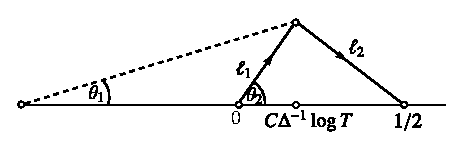
\includegraphics{figures/5.2.eps}
\end{figure}
$H \in e$ $\theta_1 = (T \log T)^{-1}$, $\theta_2 \asymp \Delta (T
\log^2 T)^{-1}$, $C >0$ is a large constant and $\xi > 0$ (the case
$\xi < 0$ is similar). On $\ell_1$ we have $x^{i\xi} \ll \exp (-C \xi
\Delta / (T \log^2 T))$, and on $\ell_2$ we have $|x| \geq C
\Delta^{-1} \log T$. Hence we obtain, for some $C' > 0$, 
\begin{equation}
\Xi^\circ (P_T ; i\xi) \ll \exp \left(-C' \frac{|\xi|\Delta}{T \log^2 T} \right) + \exp (-C'\log^2 T),\label{c5:eq5.131}
\end{equation}
providing $|\xi| \leq C_1 T \log T$. Therefore
\begin{align}
& (\Delta \sqrt{\pi})^{-1} \int\limits^\infty_{-\infty} \left|\zeta
  \left(\frac{1}{2} + iT + it \right)\right|^4 e^{-(t/\Delta)^2}
  dt\label{c5:eq5.132}\\ 
& = F_0 (T,\Delta) + \frac{1}{\pi} \int\limits^{CT\Delta^{-i} \log^3
  T}_{-CT \Delta^{-1} \log^3 T} \frac{|\zeta (\frac{1}{2} + i
  \xi)|^6}{|\zeta(1+2i\xi)|^2} \theta (\xi; T,\Delta) d \xi\notag\\ 
&\quad + \sum\limits_{x_j \leq C T \Delta^{-1} \log^3 T} \alpha_j
H^3_j \left(\frac{1}{2} \right) \theta (x_j ; T,\Delta) + o (T^{-1}
\log^2 T),\notag 
\end{align}
and henceforth we restrict $\Delta$ to the range
\begin{equation}
T^{\frac{1}{2}} \log^{-A} T \leq \Delta \leq T \exp (-\sqrt{\log T}),
\label{c5:eq5.133} 
\end{equation}\pageoriginale
with $A>0$ an arbitrary, but fixed constant. One can consider also the
values of $\Delta$ outside this range, but for all practical purposes
the range (\ref{c5:eq5.133}) appears to be sufficient. We proceed now
to evaluate 
\begin{align}
\Xi^\circ (P_T; i \xi) &=
2 \pi i \int\limits^1_0 \int\limits^{\frac{1}{2}}_0 x^{-\frac{1}{2} +
  i \xi} (1+x)^{-\frac{1}{2} + iT} (1+xy)^{-\frac{1}{2} - i \xi}
y^{-\frac{1}{2} + i \xi}\notag\\ 
&\qquad (1-y)^{-\frac{1}{2}+i\xi} e^{-\frac{1}{4}
  \Delta^2 \log^2 (1+x) } dx \; dy \label{c5:eq5.134}
\end{align}
by using the following procedure. For $|\xi| \leq \log^{3A} T$ we
integrate first over $y$ (simplifying $(1+xy)^{-\frac{1}{2} -i \xi}$
by Taylor's formula), getting essentially a beta-integral, that is,  
{\fontsize{10pt}{12pt}\selectfont
\begin{equation}
B(p,q) = \int\limits^1_0 x^{p-1} (1-x)^{q-1} dx = \frac{\Gamma(p)
  \Gamma (q)}{\Gamma (p+q)} \;\; (\re p > 0, \; \re q >
0).\label{c5:eq5.135} 
\end{equation}}

For the remaining range $\log^{3A} T \leq |\xi| \leq CT\Delta^{-1}
\log^3 T$ we use the saddle-point method, evaluating first the
integral over $x$, and then integrating over $y$. 

Thus we begin the evaluation of $\Xi^\circ (P_T;i\xi)$, supposing
$|\xi| \leq \log^{3A} T$. By (\ref{c5:eq5.134}) we have, with some
$c>0$, 
\begin{align*}
& \Xi^\circ (P_T ; i\xi) = O (e^{-clog^2 T}) + 
2 \pi i \int\limits^{\Delta^{-1} \log T}_0 x^{-\frac{1}{2} + i \xi}
(1+x)^{-\frac{1}{2} + iT} \\ 
& \qquad \exp \left(-\frac{\Delta^2}{4} \log^2 (1+x) \right) dx
\int\limits^1_0 y^{-\frac{1}{2} + i \xi} (1-y)^{-\frac{1}{2} + i \xi}
(1+xy)^{-\frac{1}{2} - i \xi} dy \\ 
& \qquad = 2 \pi i \int\limits^{\Delta^{-1} \log T}_0 x^{-\frac{1}{2}
  + i\xi } (1+x)^{-\frac{1}{2} + iT} \exp \left(-\frac{\Delta^2}{4}
\log^2 (1+x) \right) dx \\ 
& \qquad \qquad \int\limits^1_0 y^{-\frac{1}{2} + i \xi}
(1-y)^{-\frac{1}{2} + i\xi} dy +  
 2 \pi i \int\limits^{\Delta^{-1} \log T}_0 x^{-\frac{1}{2} + i\xi}
 (1+x)^{-\frac{1}{2} + iT} \\ 
& \qquad \qquad x \left(-\frac{1}{x} - i \xi \right) \exp
 \left(-\frac{\Delta^2}{4} \log^2 (1+x) \right) dx \int\limits^1_0
 y^{\frac{1}{2} + i \xi} (1-y)^{-\frac{1}{2} + i  \xi} dy\\ 
& \qquad + O \left(\int\limits^{\Delta^{-1} \log T}_0 x^{3/2}
 \log^{6A} T \cdot dx \right) + O (e^{-c\log^2 T }) = I_1 + I_2 +
 O(T^{-1}) , 
\end{align*}
say. We have
\begin{align*}
  I_1 & = 2 \pi i \int\limits^{\Delta^{-1} \log T}_0 x^{-\frac{1}{2} +
    i \xi} (1+x)^{-\frac{1}{2} + iT} \\ 
& \hspace{1cm} \exp \left(-\frac{\Delta^2}{4} \log^2 (1+x) \right) dx
  \int\limits^1_0 y^{-\frac{1}{2} + i \xi} (1-y)^{-\frac{1}{2}+ i \xi}
  dy\\ 
& = 2 \pi i  \frac{\Gamma^2 (\frac{1}{2} + i \xi)}{\Gamma(1+2i\xi)}
  \int\limits^\infty_0 x^{-\frac{1}{2} + i \xi} (1+x)^{-\frac{1}{2} +
    iT} \\ 
& \hspace{1cm}  \exp \left(-\frac{\Delta^2}{4} \log^2 (1+x)\right) dx
  + O(e^{-c\log^2 T}). 
\end{align*}\pageoriginale

Next we use
$$ 
\int\limits^\infty_{-\infty} \exp (\alpha x - \beta x^2) dx =
\sqrt{\frac{\pi}{\beta}} \exp \left(\frac{\alpha^2}{4\beta} \right)
\quad (\re \beta > 0)  
$$
to write the last integral above as
\begin{align*}
& (\Delta \sqrt{\pi})^{-1} \int\limits^\infty_0 x^{-\frac{1}{2} + i
    \xi} (1+x)^{-\frac{1}{2}+ iT} \left(\int\limits^\infty_{-\infty}
  (1+x)^{iu} e^{-(u/\Delta)^2} du \right) dx\\ 
& = (\Delta \sqrt{\pi})^{-1} \int\limits^1_0 v^{-\frac{1}{2} + i \xi}
  (1-v)^{-1-i\xi - iT} \int\limits^\infty_{-\infty} (1-v)^{-iu}
  e^{-(u/\Delta)^2} du \; dv 
\end{align*}
after change of variable $x/(1+x) =v$. This may be further written as 
\begin{align*}
& (\Delta/\sqrt{\pi})^{-1} \lim\limits_{\alpha \to -1 + 0} \int\limits^1_0 
v^{-\frac{1}{2} + i \xi} (1-v)^{\alpha-i\xi-iT} \int\limits^{\infty}_{-\infty} 
(1-v)^{-iu} e^{-(u/\Delta)^2} du \; dv\\
& = (\Delta \sqrt{\pi})^{-1} \lim\limits_{\alpha \to - 1 + 0 }
\int\limits^{\Delta \log T}_{-\Delta \log T} e^{-(u/\Delta)^2} du \\ 
& \qquad \int\limits^1_0 v^{-\frac{1}{2} + i \xi} (1-v)^{\alpha - i
  \xi  - i T - iu} dv + O (e^{-c\log^2 T}) \\ 
&= (\Delta \sqrt{\pi})^{-1} \lim\limits_{\alpha \to -1+0 }
\int\limits^{\Delta \log T}_{-\Delta \log T} e^{-(u/\Delta)^2} \cdot
\\ 
& \qquad \frac{\Gamma (\frac{1}{2} + i \xi) \Gamma (\alpha + 1 - i \xi
  - iT - iu)}{\Gamma (\alpha + \frac{3}{2} - i T - iu)} du + O
(e^{-c\log^2 T})\\ 
&= (\Delta \sqrt{\pi})^{-1} \int\limits^{\Delta \log T}_{-\Delta \log
  T} e^{-(u/\Delta)^2} \cdot \frac{\Gamma (\frac{1}{2} + i \xi) \Gamma
  (-\xi - iT- iu)}{\Gamma (\frac{1}{2} - iT - iu)} du + O (e^{-c\log^2
  T}), 
\end{align*}
where uniform convergence was used and the fact that $\xi + T + u \neq
0$ for $|u| \leq \Delta \log T$, $|\xi| \leq \log^{3A} T$. By
Stirling's formula, in the form stated after (\ref{c3:eq3.18}), we
find that  
\begin{align*}
& \frac{\Gamma (\frac{1}{2} + i \xi) \Gamma (-i \xi - iT - i
    u)}{\Gamma (\frac{1}{2} - iT - i u)} =  \Gamma \left(\frac{1}{2} +
  i \xi \right) (T + u + \xi)^{-\frac{1}{2}}\\ 
&\qquad  \exp \left\{-\frac{\pi}{2} \xi + \frac{\pi i}{4} - i \xi \log
  (T+u) + O \left(\frac{|\xi|}{T} \right) \right\} \cdot \left(1+O
  \left(\frac{1}{T} \right) \right). 
\end{align*}\pageoriginale

Since 
\begin{align*}
& \log (T + u) = \log T + \frac{u}{T} + O \left(\frac{\Delta^2 \log^2
    T}{T^2} \right), \\ 
& (T + u + \xi)^{-\frac{1}{2}} = T^{-\frac{1}{2}} + O (T^{-3/2}\Delta
  \log T) 
\end{align*}
and $\Delta \leq T \exp (\sigma \sqrt{\log T})$, it follows that 
\begin{align*}
& \frac{\Gamma (\frac{1}{2} + i \xi ) \Gamma (-i\xi - iT - iu)}{\Gamma
    (\frac{1}{2} - i u - iT)} = \Gamma \left(\frac{1}{2} + i \xi
  \right) \\ 
& \qquad e^{\frac{1}{4} \pi i - \frac{1}{2} \pi \xi}  T^{-\frac{1}{2}
    - i \xi} \cdot \left\{1+ 0 \left(\exp \left(-\frac{1}{2}
  \sqrt{\log T} \right) \right) \right\}. 
\end{align*}

This means that the last expression is negligible if $\xi > 0$ and
$\xi$ is large, in which case $\Gamma (\frac{1}{2} + i \xi) \asymp
\exp (-\frac{1}{2} \pi\xi)$. Therefore 
$$ 
I_1 = 2 \pi i \frac{\Gamma^3 (\frac{1}{2} + i \xi)}{\Gamma (1+ 2 i
  \xi)} e^{\frac{1}{4} \pi i - \frac{1}{2} \pi \xi} T^{-\frac{1}{2} -
  i \xi} \left\{ 1+ 0 \left(\exp \left(-\frac{1}{2} \sqrt{\log T}
\right) \right)\right\}, 
$$
and by the same method it is established that
$$
I_2 \ll T^{-\frac{1}{2}} \exp \left(-\frac{1}{2} \sqrt{\log T} \right). 
$$

Hence uniformly for $|\xi| \leq \log^{3A} T$ we have
{\fontsize{9pt}{11pt}\selectfont
\begin{equation}
\Xi^\circ (P_T; i \xi) = 2 \pi ie^{\frac{1}{4} \pi i - \frac{1}{2} \pi
  \xi} \frac{\Gamma^3 (\frac{1}{2} + i \xi)}{ \Gamma (1+ 2 i \xi)}
T^{-\frac{1}{2} - i \xi} \left\{1+ O \left(\exp \left(-\frac{1}{2}
\sqrt{\log T} \right) \right)\right\}. 
\label{c5:eq5.136}
\end{equation}}

It may be remarked that the expression in (\ref{c5:eq5.136}) can be
integrated in applications whenever this is needed. Now we suppose
additionally 
\begin{equation}
D < |\xi| \leq \log^{3A} T,\label{c5:eq5.137}
\end{equation}
where $D >0$ is a large constant. Then we use again Stirling's formula
to obtain 
\begin{equation}
\Xi^\circ (P_T ; i \xi) \ll T^{-\frac{1}{2}} e^{-\pi \xi} \quad (\xi > 0),\label{c5:eq5.138}
\end{equation}
and 
{\fontsize{9pt}{11pt}\selectfont
\begin{equation}
\Xi^\circ (P_T ; i \xi) = - 4 \pi^2 2^{-\frac{1}{2}}( T
|\xi|)^{-\frac{1}{2}} \exp (i \xi \log |\xi| - i \xi \log (4 eT))
\cdot \left(1+O \left(\frac{1}{|\xi|} \right) \right)\label{c5:eq5.139}
\end{equation}}
for $\xi < 0$. Finally from (\ref{c5:eq5.138}) and (\ref{c5:eq5.139})
we can obtain an asymptotic formula for $\theta (\xi; T,\Delta)$ when
(\ref{c5:eq5.137}) holds. On using (\ref{c5:eq5.117}) and
(\ref{c5:eq5.118}) it is seen that  
\begin{align}
& \theta (\xi;T,\Delta) = 2 \re \{\Psi (P_T;i\xi) - \Phi (P_T; i
  \xi)\}\label{c5:eq5.140}\\ 
& = \frac{1}{4\pi} \re \left\{ \left( \frac{1}{sh (\pi \xi)} - i
  \right) \Xi (P_T ; i \xi) - \left(\frac{1}{sh (\pi \xi)} + i \right)
  \Xi (P_T; - i\xi)\right\}\notag\\ 
& = \frac{1}{4 \pi} \im \left\{ \Xi^\circ (P_T ; i \xi) + \Xi^\circ
  (P_T;-i\xi) \right\} + O (T^{-\frac{1}{2}} |\xi|^{-1}).\notag  
\end{align}\pageoriginale

Thus $\theta (\xi;T,\Delta) \ll |\xi|^{-\frac{1}{2}} T^{-\frac{1}{2}}$
in the continuous spectrum, making the total contribution of the
continuous spectrum $\ll T^{-\frac{1}{2}} \log^C T$ for $|\xi| \leq
\log^{3A} T$. On the other hand, in the discrete spectrum one has to
take $\xi > 0$, so that the main contribution to $\theta (x_j;
T,\Delta)$ (with error which is $0(T^{-\frac{1}{2}} x^{-1}_j)$) will
be 
\begin{align*}
& \frac{1}{4\pi} \im \{\Xi^\circ (P_T;- i x_j)\}\\
& = - \pi (2 T x_j)^{-\frac{1}{2}} \sin \left(x_j \log \frac{4eT}{x_j}
  \right) = \pi (2T x_j)^{-\frac{1}{2}} \sin \left( x_j \log
  \frac{x_j}{4 eT}\right). 
\end{align*}

Then  we can, in view of $\Delta \leq T \exp (-\sqrt{\log T})$, $x_j
\leq \log^{3A} T$, insert the exponential factor $\exp (-(\Delta x_j/
2T)^2)$ in the relevant term in (\ref{c5:eq5.132}), making a
negligible error. This is done, because these (harmless) factors are
present in the series appearing in Theorem \ref{c5:thm5.2} and Theorem
\ref{c5:thm5.3}. Hence it remains to consider the ranges $|\xi| \leq
D$ and $\log^{3A} T \leq |\xi| \leq CT\Delta^{-1} \log^3T$. In the
range $|\xi| \leq D$ we trivially have $\Xi^\circ (P_T; i\xi) \ll
T^{-\frac{1}{2}}$, so that the contribution to both the continuous and
discrete spectrum is $\ll T^{-\frac{1}{2}}$, more than required by
Theorem \ref{c5:thm5.2}.  

We turn now to the range
\begin{equation}
\log^{3A} T \leq |\xi| \leq CT\Delta^{-1} \log^3
T,\label{c5:eq5.141} 
\end{equation}
provided that (\ref{c5:eq5.133}) holds. We rewrite (\ref{c5:eq5.134})
as  
\begin{equation}
\Xi^\circ (P_T; i\xi) = 2 \pi i \int\limits^1_0 y^{-\frac{1}{2} + i
  \xi} (1-y)^{-\frac{1}{2} + i \xi} S(y;\xi) dy,
\label{c5:eq5.142} 
\end{equation}
where
\begin{equation}
S (y;\xi) : =\int\limits^{\frac{1}{2}}_0 x^{-\frac{1}{2} + i \xi}
(1+x)^{-\frac{1}{2}+ iT} (1+xy)^{-\frac{1}{2} - i \xi} e^{-\frac{1}{4}
  \Delta^2 \log^2 (1+x)} dx, 
\label{c5:eq5.143}
\end{equation}
and proceed to evaluate by the saddle-point method first $S(y;\xi)$,
and then $\Xi^\circ$ itself. First we show that, in case $\xi > 0$ and
(\ref{c5:eq5.141}) holds,\pageoriginale the contribution of $S(y;\xi)$
is negligible uniformly in $y$. Namely we replace the segment of
integration $[0,\frac{1}{2}]$ by $L_1 \cup L_2$, as follows: 

\begin{figure}[H]
\centering
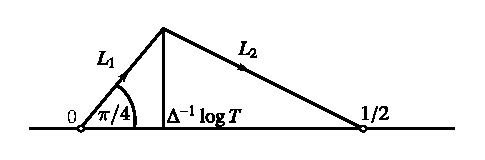
\includegraphics{figures/5.3.eps}
\end{figure}

On $L_1$ we have $x^{i \xi} \ll \exp \left(-\frac{1}{4} \pi \xi
\right)$, hence the integral over $L_1$ is $\ll \exp
\left(-\dfrac{\pi}{8} \xi \right)$. On $L_2$ we have $|x| \gg
\Delta^{-1} \log T$, consequently we obtain, for $\xi > 0$, 
\begin{equation}
\Xi^\circ (P_T;i\xi) \ll \exp \left(-\frac{\pi}{8} \xi \right) + \exp
(-C_1 \log^2 T).\label{c5:eq5.144} 
\end{equation}

In case $\xi  < 0$ write
$$ 
S(y;\xi) = \int\limits^{\frac{1}{2}}_0 x^{-\frac{1}{2}}
(1+x)^{-\frac{1}{2}} \exp \left(-\frac{\Delta^2}{4} \log^2 (1+x)
\right) \exp (if  (x)) dx, 
$$
where 
$$
f(x) = f(x;\xi, T, y): = \xi \log x + T \log (1+x) - \xi \log (1+ xy),  
$$
so that 
$$
f'(x) = \frac{\xi}{x} + \frac{T}{1+x} - \frac{\xi y}{1+ xy} , f''(x) =
-\frac{\xi}{x^2} -\frac{T}{(1+x)^2} + \frac{\xi y^2}{ (1+ xy)^2}. 
$$

The saddle point is the solution of the equation $f'(x_\circ) = 0$, giving
\begin{align}
x_\circ & = \frac{2|\xi|}{T - |\xi| + \left((T - |\xi|)^2 + 4 T
  y\xi\right)^{\frac{1}{2}}}\notag\\[5pt] 
& = \frac{|\xi|}{T -|\xi|} \left(1 -\frac{y|\xi|}{T} + O
\left(\frac{\xi^2}{T^2}\right)\right)  \sim
\frac{|\xi|}{T}.\label{c5:eq5.145} 
\end{align}

We can now evaluate $S(y;\xi)$ by a general result on exponential
integrals, like Theorem \ref{c2:thm2.3}. This will be sufficient for
the proof of Theorem \ref{c5:thm5.2} and the first part of Theorem
\ref{c5:thm5.3}. On the other hand, we may use a special contour,
suited to the particular structure of the integral $S(y;\xi)$, and
evaluate $S(y;\xi)$ from first principles. The latter approach, which
is naturally more delicate, leads to slightly better error terms and
enables one to deduce the second part of Theorem \ref{c5:thm5.3}.  

Thus\pageoriginale we shall first use Theorem \ref{c2:thm2.3}, but
before it is applied we shall truncate $S(y;\xi)$. So consider 
\begin{align*}
& \int\limits^{T^{-1}}_0 x^{-\frac{1}{2}} (1+x)^{-\frac{1}{2}} \exp
  \left(-\frac{\Delta^2}{4} \log^2 (1+x) \right) \exp  (if (x)) dx\\ 
& =  \sum\limits^\infty_{k=0} \ \int\limits^{T^{-1} 2^{-k}}_{T^{-1}
    2^{-k-1}} \ldots  = \sum\limits^\infty_{k=0} I(k), 
\end{align*}
say. In each $I(k)$ we have $f'(x) \gg |\xi| /x$, hence by Lemma
\ref{c2:lem2.1} 
$$
I(k) \ll (T^{-1} 2^{-k})^{-\frac{1}{2}} (|\xi| T2^k)^{-1} \ll
|\xi|^{-1} T^{-\frac{1}{2}} 2^{-\frac{1}{2}} k, 
$$
and consequently
$$
\int\limits^{T^{-1}}_0 x^{-\frac{1}{2}} (1+x)^{-\frac{1}{2}} \exp
\left(-\frac{\Delta^2}{4} \log^2 (1+x)\right) \exp (if(x)) dx \ll
\quad |\xi|^{-1} T^{-\frac{1}{2}} 
$$

Also we have trivially
\begin{align*}
& \int\limits^{\frac{1}{2}}_{|\xi|^{1/2} (10T)^{-1/2}}
  x^{-\frac{1}{2}} (1+x)^{-\frac{1}{2}} \exp \left(
  -\frac{\Delta^2}{4} \log^2 (1+x)\right) \exp (if (x)) dx\\ 
& \qquad \ll \exp \left(-\frac{\Delta^2 |\xi|}{100 T} \right) \ll \exp
  \left(-\frac{|\xi| \log^{-2A} T}{100} \right) \ll \exp
  \left(-\frac{\log^A T}{100}  \right) 
\end{align*}
in view of (\ref{c5:eq5.141}), and thus the integral is negligible if
$A >1$, which may be assumed. In the remaining integral 
$$ 
I : = \int\limits^{|\xi|^{1/2} (10T)^{-1/2}}_{T^{-1}} x^{-\frac{1}{2}}
(1+x)^{-\frac{1}{2}} \exp \left(-\frac{\Delta^2}{4} \log^2  (1+x)
\right) \exp (if (x)) dx 
$$
we have $f'(x) \ll \min (|\xi| x^{-1}, T)$, $f''(x) \gg |\xi|
x^{-2}$. To evaluate I we apply Theorem \ref{c2:thm2.3} with $a =
T^{-1}$, $b = |\xi|^{\frac{1}{2}} (10T)^{-\frac{1}{2}}$, $\Phi(x) =
x^{-\frac{1}{2}} \exp (-C \Delta^2 x^2)$, $\mu (x) = x/10$,
$\varphi(x) = x^{-\frac{1}{2}} (1+x)^{-\frac{1}{2}} \exp
\left(-\frac{\Delta^2}{4} \log^2 (1+x)  \right)$ $F (x) =\break \min (|\xi|,
Tx)$.  We have $|f''(z)|^{-1} \ll x^2 |\xi|^{-1} \ll \mu^2 (x)
F^{-1}(x)$ trivially if $F(x) = |\xi|$, and $x^2 |\xi|^{-1} \ll x^2
T^{-1} x^{-1} \ll \mu^2 (x) F^{-1} (x)$ if $x \leq |\xi|T^{-1}$. For
the error terms we obtain 
\begin{align*}
& \Phi_a \left(|f'_a| + {f''}_a^{\frac{1}{2}}\right)^{-1} \ll T^{\frac{1}{2}}
  (|\xi|T)^{-1} = |\xi|^{-1} T^{-\frac{1}{2}},\\ 
& \Phi_b \left(|f'_b| + f''^{\frac{1}{2}}_b\right)^{-1} \ll e^{-c\log^2
    T},\quad \Phi_0 \mu_0 F^{-3/2}_0 \ll |\xi|^{-1} \cdot T^{-\frac{1}{2}},  
\end{align*}\pageoriginale
and the contribution of the exponential error term in Theorem
\ref{c2:thm2.3} is clearly negligible. Therefore Theorem
\ref{c2:thm2.3} gives 
\begin{align*}
& I = \sqrt{2\pi} \varphi_0 (f''_0)^{-\frac{1}{2}} \exp \left(iT \log 
  (1+x_0) + i\xi \log \frac{x_0}{1+x_0y} + \frac{i\pi}{4}\right)\\ 
&\qquad {}+ O \left(|\xi|^{-1} T^{-\frac{1}{2}}\right)= \sqrt{2\pi}
  T^{-\frac{1}{2}} \exp \left(- \left(\frac{\Delta 
    \xi}{2T} \right)^2 \right) \\ 
&\qquad \exp \left(iT \log (1+x_0) + i \xi \log \frac{x_0}{1+x_0 y}  +
  \frac{i\pi}{4} \right) + O \left(|\xi|^{-1} T^{-\frac{1}{2}}\right). 
\end{align*}

Since $\xi < 0$ we also obtain, by using (\ref{c5:eq5.145}),
$$
 T \log (1+ x_0) + \xi \log \frac{x_0}{1+x_0 y} = \xi \log
 \frac{|\xi|}{eT} + \left(y-\frac{1}{2} \right) \frac{\xi^2}{T} + O
 \left(\frac{|\xi|^2}{T^2} \right), 
$$
which gives
\begin{align*}
I & = \sqrt{2\pi} T^{-\frac{1}{2}} \exp \left(- \left(\frac{\Delta \xi}{2T} \right)^2 \right) \exp \left(i\xi \log \frac{|\xi|}{eT} + i \left(y-\frac{1}{2} \right) \frac{\xi^2}{T} + \frac{i\pi}{4} \right)\\
&\qquad +  O\left(|\xi|^3 T^{-5/2}\right) + O\left(|\xi|^{-1}
T^{-\frac{1}{2}}\right). 
\end{align*}

Then 
\begin{align}
\Xi^\circ (P_T ; i\xi) & = O \left(|\xi|^3 T^{-5/2}\right) +
O\left(|\xi|^{-1} T^{-\frac{1}{2}}\right) +  
(2\pi)^{3/2} e^{\frac{3}{4} \pi i}
T^{-\frac{1}{2}}\label{c5:eq5.146}\\ 
& \qquad \exp \left(i\xi \log \frac{|\xi|}{eT} - \frac{i\xi^2}{2T}
\right) e^{-(\frac{\Delta \xi}{2T})^2} \cdot \int\limits^1_0
(y(1-y))^{-\frac{1}{2}}\notag\\ 
& \qquad \exp \left\{ i \xi \log (y (1-y)) + \frac{i \xi^2}{T}
y\right\} dy.\notag 
\end{align}

The last integral may be truncated at $|\xi|^{-2}$ and $1-|\xi|^2$
with an error of $O(|\xi|^{-1})$. The remaining integral 
\begin{align*}
& J : = \int\limits^{1-|\xi|^{-2}}_{|\xi|^{-2}}
  (y(1-y))^{-\frac{1}{2}} \exp (i\bar{f}(y)) dy,\\ 
& \bar{f} (y) = \bar{f} (y; \xi, T): =  \xi \log (y (1-y)) +
  \frac{\xi^2}{T} y 
\end{align*}
may be evaluated again by Theorem \ref{c2:thm2.3}. We have 
$$ 
\bar{f}'(x) = \frac{\xi}{x} - \frac{\xi}{1-x} + \frac{\xi^2}{T},  \;
\bar{f}'' (x) = - \frac{\xi}{x^2} -\frac{\xi}{(1-x)^2}, 
$$
and the saddle point $x_\circ$ satisfies $\bar{f}'(x_\circ) = 0$,
whence 
$$ 
x_\circ = \left(1-\frac{\xi}{2T} + \left(1+ \frac{\xi^2}{4T^2}
\right)^{\frac{1}{2}} \right)^{\cdot -1} = \frac{1}{2} +
\frac{\xi}{8T} -\frac{\xi^3}{128 T^3} + O \left(\frac{|\xi|^5}{T^5}\right).  
$$

The error\pageoriginale terms from Theorem \ref{c2:thm2.3} will be all
$\ll \xi^{-2}$. Thus with $\varphi(x) = (x (1-x))^{-\frac{1}{2}}$ we
obtain 
\begin{align*}
J &= \sqrt{2\pi} \varphi_\circ (\bar{f}''_\circ) \exp \left(if_\circ +
\frac{i\pi}{4} \right) + O (\xi^{-2})\\ 
&= \pi^{\frac{1}{2}} e^{\frac{1}{4} \pi i} |\xi|^{-\frac{1}{2}}
\left\{1+O\left(|\xi| T^{-1}\right) + O \left(|\xi|^3
T^{-2}\right)\right\}\\ 
&\qquad\exp \left(-i\xi \log 4 +
\frac{i\xi^2}{T} \right) + O (\xi^{-2}). 
\end{align*}

Inserting the expression for $J$ in (\ref{c5:eq5.146}) we obtain
\begin{align}
\Xi^\circ (P_T;i\xi) &  = 
- 2^{3/2} \pi^2 (|\xi|T)^{-\frac{1}{2}} \exp \left(i\xi \log
\frac{|\xi|}{4 eT} \right)\label{c5:eq5.147}\\  
& \qquad \exp \left(\left(-\frac{\Delta \xi}{2T} \right)^2 \right)
\left(1+O\left(|\xi| T^{-1}\right) + O \left(|\xi|^3
T^{-2}\right)\right)\notag\\ 
& \qquad + O\left(|\xi|^3 T^{-{5/2}}\right) +  O \left(|\xi|^{-1}
T^{-\frac{1}{2}}\right) \quad (\xi < 0), \notag
\end{align}
provided that (\ref{c5:eq5.141}) holds. The error terms
$O(|\xi|T^{-1})$ and $O(|\xi|^3 T^{-2})$ in (\ref{c5:eq5.147}) will
make a negligible contribution. The main term in (\ref{c5:eq5.147}) is
the same main term as in (\ref{c5:eq5.139}), only with the additional
factor $\exp (-(\Delta \xi/2T)^2)$. Hence the analysis concerning the
main term in\break (\ref{c5:eq5.147}) will be as in the previous case. To
deal with the remaining two error terms in (\ref{c5:eq5.147}) we shall
use the bounds 
\begin{equation}
\int\limits^T_0 \left|\zeta \left(\frac{1}{2} + it \right)\right|^6 dt
\ll  T^{5/4} \log^{29/4} T \label{c5:eq5.148}
\end{equation}
and
\begin{equation}
\sum\limits_{x_j \leq x} \alpha_j \left|H^3_j \left(\frac{1}{2} \right)\right|
\ll x^2 \log^C x.  \label{c5:eq5.149}
\end{equation}

The last bound (with $C =\frac{1}{2} (B+1)$) follows on using the
Cauchy-Schwarz inequality and the bounds 
\begin{align}
& \sum\limits_{x_j \leq x} \alpha_j H^2_j \left(\frac{1}{2} \right)
  \ll x^2 \log x, \label{c5:eq5.150}\\  
& \sum\limits_{x_j \leq x} \alpha_j H^4_j (\frac{1}{2}) \ll x^2 \log^B
  x.\label{c5:eq5.151} 
\end{align}

Note that (\ref{c5:eq5.150}) is a weak consequence of
(\ref{c5:eq5.55}), while (\ref{c5:eq5.151}) has been claimed by
N. Kuzmetsov. A proof was found recently by Y. Motohashi, which shows
that actually (\ref{c5:eq5.151}) holds with $B =20$. 
Therefore\pageoriginale on using (\ref{c5:eq5.148}) it follows that
the contribution of the error terms $O(|\xi|^3 T^{-5/2})$ and
$O(|\xi|^{-1} T^{-\frac{1}{2}})$ to the continuous spectrum
(i.e. integral) in (\ref{c5:eq5.132}) is negligible. The contribution
of these error terms to the discrete spectrum (i.e. sum) in
(\ref{c5:eq5.132}) is, by (\ref{c5:eq5.149}) and partial summation, 
\begin{align*}
&\ll \sum\limits_{x_j \leq C T \Delta^{-1} \log^3 T} \alpha_j \left|H^3_j 
  \left(\frac{1}{2} \right)\right| \left(x^3_j T^{-5/2} + x^{-1}_j
  T^{-\frac{1}{2}}\right)\\   
&\ll \left(T\Delta^{-1} \log^3 T\right)^5 T^{-5/2} \log^C T +
  \left(T\Delta^{-1} \log^3 T\right) T^{-\frac{1}{2}} \log^C T\\
&\ll (\log T)^{D(A)} 
\end{align*}
with $D(A) = 15 + 5A + C$, providing that (\ref{c5:eq5.137})
holds. This established then Theorem \ref{c5:thm5.2} in view of
(\ref{c5:eq5.11}). 

We pass now to the discussion of the proof of the first part of
Theorem \ref{c5:thm5.3}. We integrate Theorem \ref{c5:thm5.1} over $T$
for $V \leq T \leq 2V$. First we note that from (\ref{c5:eq5.24}) we
have 
\begin{align*}
& \int\limits^{2V}_V M \left(s, \frac{1}{2} - iT;\Delta \right) dT\\
& = - i \int\limits^\infty_0 x^{s-1} (1+x)^{-\frac{1}{2} + iV} \frac{(1+x)^{iV} -1}{\log (1+x)} \exp \left(-\frac{\Delta^2}{4} \log^2 (1+x) \right) dx. 
\end{align*}

If $\re s >1$ and $T^{\epsilon} \leq \Delta \leq T \exp (-\sqrt{\log
  T})$ the right-hand side is  
$$
\ll \Delta^{1-\re s} e^{-|\im s|/V}
$$
similarly as in the proof of (\ref{c5:eq5.121}). Hence we obtain
$$
\int\limits^{2V}_V \Lambda (k;T,\Delta) dT \ll
\begin{cases}
\Delta^{1-k}  &  k \leq C,\\
(k\Delta)^{-C_1} &  k > C,
\end{cases}
$$
for any fixed $C_1 >0$. This means that the contribution of the
holomorphic part in (\ref{c5:eq5.10}) to the integral in
(\ref{c5:eq5.13}) is negligible. From the formula (see Section
\ref{c5:sec5.1}) 
\begin{equation*}
\frac{\Gamma^{(k)} (s)}{\Gamma(s)}  = \sum\limits^k_{j=0} b_{j,k} (s)
\log^j s + c_{-1,k} s^{-1} + \ldots + c_{-r, k} s^{-r}  + O_r
\left(|s|^{-r-1}\right) 
\end{equation*}
it follows\pageoriginale that, for a suitable polynomial $R_4 (y)$ of
degree four in $y$, 
$$
\int\limits^{2V}_V F_0 (T,\Delta) dT = V R_4 (\log V) + O(\Delta
\log^5 V), 
$$
hence both (\ref{c5:eq5.13}) and (\ref{c5:eq5.14}) will contain the
error term $O(\Delta \log^5 V)$. 

The proof of (\ref{c5:eq5.13}) resembles the foregoing proof, only in
(\ref{c5:eq5.134}) we integrate for $V \leq T \leq 2V$, and eventually
we shall replace $V$ by $V 2^{-j}$ and sum over $j = 1,2,\ldots$. We
have now also to consider the additional factor $i^{-1} \log^{-1}
(1+x) \sim i^{-1} x^{-1}$ at $x = x_0$, which appears in the integrals
in (\ref{c5:eq5.134}) after integration over $T$. Since $x_0 \sim
|\xi|T^{-1}$, the factor $i^{-1} T |\xi|^{-1}$ will be essentially
reproduced in the whole analysis, both in the main term and error
terms. Thus we shall have, as the analogue of (\ref{c5:eq5.147}), 
\begin{align*}
&\int\limits^{2V}_V \Xi^\circ (P_T;i\xi) d T = O\left(|\xi|^2
  V^{-3/2}\right) + O\left(|\xi|^{-2} V^{1/2}\right)\\ 
&\qquad {}+\left| i2^{3/2} \pi^{2}|\xi|^{-3/2} T^{\frac{1}{2}} \exp
  \left(i\xi \log \frac{|\xi|}{4eT} \right) e^{-(\Delta \xi / 2 T)^2}
\right|^{2V}_V\\
&\qquad\qquad\left(1+O\left(|\xi|V^{-1}\right) + O \left(|\xi|^3
V^{-2}\right)\right),  
\end{align*}
and the factor $i$ accounts for the change of sine into cosine in
Theorem \ref{c5:thm5.3}. The error terms above will all contribute a
total of $O(V^{\frac{1}{2}} \log^{D(A)}V )$, and the first part of
Theorem \ref{c5:thm5.3} follows, since similar arguments apply to
(\ref{c5:eq5.136}). 

As mentioned earlier, there is a possibility to evaluate $S(y;\xi)$ in
(\ref{c5:eq5.143}) (for $\xi < 0$ and (\ref{c5:eq5.141}) being true)
directly by treating it as a complex integral, choosing a suitable
contour in the $x$-plane to replace the segment of integration
$[0,\frac{1}{2}]$. Such an evaluation is necessary for the proof of
the second part of Theorem \ref{c5:thm5.3}, namely
(\ref{c5:eq5.14}). This was the approach used originally by Motohashi,
who replaced the segment $[0,\frac{1}{2}]$ by $\ell_1 \cup \ell_2 \cup
\ell_3 \cup \ell_4$. Here $\ell_1,\ell_2, \ell_3, \ell_4$ denote
segments formed by the points $0$, $\frac{1}{2} x_0 (1-i)$,
$x_0(1+\epsilon + \epsilon i)$, $\Delta^{-1} \log^2 T + x_0 \epsilon
i, \frac{1}{2}$ respectively, and $\epsilon > 0$ is a small
constant. On $\ell_1$ the integrand of $S(y;\xi)$ is, uniformly in~$y$, 
\begin{align*}
& \ll |x|^{-\frac{1}{2}} \exp \left( -\frac{\pi}{4} |\xi| + T \arc\tan
  \frac{x_0}{2+x_0} + |\xi| \arc \tan \frac{x_0 y}{2+x_0 y}
  \right)\\ 
&\ll |x|^{-\frac{1}{2}} \exp \left(-\frac{1}{5} |\xi| \right) 
\end{align*}\pageoriginale
since $x_0 \sim |\xi| T^{-1}$. Hence the contribution of $\ell_1$ is
negligible if, say, $A > 1/3$ in (\ref{c5:eq5.141}). Clearly the
contribution of $\ell_4$ can also be neglected. As for $\ell_3$, let
$Q = x_0(1+u+\epsilon + \epsilon i)$ with $u \geq 0$. The for $0 \leq
y \leq 1$, $u \geq 0$ the integrand of $S(y;\xi)$ at $Q$ is uniformly 
\begin{align}
& \ll |x|^{-\frac{1}{2}} \exp \left(|\xi| \arc \tan
  \frac{\epsilon}{1+u+\epsilon} - T \arc \tan \frac{x_0
    \epsilon}{1+x_0 (1+u+\epsilon)}  \right.\notag\\ 
& \qquad \left.  - |\xi| \arc \tan \frac{y x_0 \epsilon}{1+ y x_0
    (1+u+ \epsilon)} \right) 
\ll |x|^{-\frac{1}{2}} \exp \left(-\frac{\epsilon^2}{2} |\xi| \right)
\label{c5:eq5.152}
\end{align}
if $\epsilon$ is sufficiently small. Thus the contribution on $\ell_3$
will be also negligible if $A$ in (\ref{c5:eq5.141}) is large enough.  

On $\ell_2$ we may use (\ref{c5:eq5.152}) with $u=0$ and $\epsilon $ a
small, positive constant. It follows that we have $x = x_0 + rx_0$,
$dx = x_0 dr$, where $r$ is the variable that runs over the segment
$\left[-\epsilon e^{\frac{1}{4} \pi i}, \epsilon e^{\frac{1}{4} \pi i}
  \right]$. However, if we restrict $r$ to the segment $[-|\xi|^{-2/5}
  e^{\frac{1}{4} \pi i}, |\xi|^{-2/5} e^{\frac{1}{4} \pi i}]$ then the
integrand on the remaining two segments of $\ell_2$ is bounded by the
last bound in (\ref{c5:eq5.152}) with $\epsilon = |\xi|^{-2/5}$. Hence
we have a total error which is 
\begin{equation}
\ll |x|^{-\frac{1}{2}} \exp \left(-C'|\xi|^{1/5}\right) \quad (C' >
0),\label{c5:eq5.153} 
\end{equation}
and this is certainly negligible if $A \geq 2$ in
(\ref{c5:eq5.141}). Therefore it follows that, for $\xi < 0$ and an
absolute 0-constant, 
{\fontsize{10pt}{12pt}\selectfont
\begin{align}
S(y;\xi) & = O\left(\exp \left(-C'|\xi|^{1/5}\right)\right) + 
\left(\frac{x_0}{(1+x_0) (1+x_0 y)} \right)^{\frac{1}{2}}\notag\\
& \quad \times \exp \left(-\frac{\Delta^2}{4} \log^2 (1+x_0) \right)
\exp \left(iT \log (1+x_0) + i \xi \log \frac{x_0}{1+x_0y}
\right)\notag\\  
& \quad \times\int\limits^{|\xi|^{-2|5} e^{\pi i /
    \mu}}_{-|\xi|^{-2/5} e^{\pi i /\mu}} (1+r)^{-\frac{1}{2}} \left(1+
\frac{x_0 yr}{1+x_0y} \right)^{-\frac{1}{2}} \left(1+\frac{x_0
  r}{1+x_0} \right)^{-\frac{1}{2}}\notag\\ 
& \quad \times\exp \left\{ -\frac{\Delta^2}{4} \left(2\log (1+x_0)
\log \left(1+\frac{x_0r}{1+x_0} \right)\right.\right. \notag\\ 
& \quad \left. \left. + \log^2 \left(1+\frac{x_0r}{1+x_0} \right)
\right)  + i \sum\limits^\infty_{j=2} a_j r^j\right\} dr .
\label{c5:eq5.154}
\end{align}}

Here we have, by Taylor's formula,
$$
a_j = \frac{x_0^j f^{(j)} (x_0)}{j!} = O_j (|\xi|), 
$$\pageoriginale
and the term with $j=1$ vanishes because $x_0$ is the saddle point of
$f(x)$, that is, $f'(x_0) = 0$. Since 
$$
f''(x) = - \frac{\xi}{x^2} - \frac{T}{(1+x)^2} + \frac{\xi
  y^2}{(1+xy)^2},  
$$
it follows that
$$ 
a_2 = \frac{|\xi|}{2} \left( 1+ \frac{Tx^2_0}{\xi (1+x_0)^2} -
\left(\frac{x_0 y}{1+x_0y} \right)^2 \right) = \frac{|\xi|}{2} \left(
1+ \frac{\xi}{T} + O \left( \frac{\xi^2}{T^2}\right)\right). 
$$

With the change of variable $r = e^{\frac{1}{4} \pi i}
a^{-\frac{1}{2}}_2 u$ the last integral above is equal to  
\begin{gather*}
e^{\frac{1}{4} \pi i} a^{-\frac{1}{2}}_2 \int\limits^{A_\xi}_{-A_\xi}
\left(1+e^{\frac{1}{4} \pi i} a^{-\frac{1}{2}}_2
u\right)^{-\frac{1}{2}}  (1+ \ldots)^{-\frac{1}{2}}
(1+\ldots)^{-1/2}\\ 
\exp \left(-\frac{\Delta^2}{4} (2\log \ldots) \right) \exp \left(-u^2
+ ia_3 e^{\frac{3}{4} \pi i} a^{-3/2}_2 u^3 - ia_4 a^{-2}_2 u^4+
\ldots \right) du, 
\end{gather*}
where $A_\xi \sim\frac{1}{2} |\xi|^{1/10}$ as $T \to
\infty$. Expanding the last exponential into its Taylor series it is
seen that this becomes 
\begin{align*}
& I (0) + \sum\limits^\infty_{j=3} b_j I (j), \quad b_j \ll
  |\xi|^{1-\frac{1}{2} j},\\ 
& I(j) = e^{\frac{1}{4} \pi i} a^{-\frac{1}{2}}_2
  \int\limits^{A_\xi}_{-A_\xi} \left(1+e^{\frac{1}{4} \pi i}
  a^{-\frac{1}{2}}_2 u\right)^{-\frac{1}{2}} (1+ \ldots)^{-\frac{1}{2}} (1+
  \ldots)^{-\frac{1}{2}} \\ 
& \exp \left( -\frac{\Delta^2}{4} \left(2\log \ldots + \log^2 \left(1+
  \frac{x_0 r}{1+x_0} \right)\right) \right) \cdot u^j e^{-u^2} du. 
\end{align*}

We truncate the series $\sum\limits^\infty_{j=3}$ at $j = J$ so large
that the trivial estimation of the terms with $j > J$ makes a total
contribution of order $O(T^{-\frac{1}{2}})$. The integrals $I(j)$ for
$j \geq 3$ will make the same type of contribution as $I(0)$, only
each will be by a factor of $|\xi|^{1-\frac{1}{2}j}$ smaller than
$I(0)$. Thus we may consider only $I(0)$ in detail. We have  
\begin{align*}
I(0) & = e^{\frac{1}{4} \pi i} a^{-\frac{1}{2}}_2
\int\limits^{A_\xi}_{-A_\xi} \left(1+e^{\frac{1}{4} \pi i}
a^{-\frac{1}{2}}_2 u\right)^{-\frac{1}{2}} \left(1+\frac{x_0
  ye^{\frac{1}{4} \pi i} a^{-\frac{1}{2}_2} u}{1+x_0 y}
\right)^{-\frac{1}{2}}\\ 
& \qquad \left(1+  \frac{x_0 e^{\frac{1}{4} \pi i }a^{-\frac{1}{2}}_2
  u}{1+x_0}\right)^{-\frac{1}{2}} \times 
\exp \left\{ - \left(\frac{\Delta}{2} \right)^2  (2\log (1+x_0) \log
\right. \\ 
& \qquad \left.  \left(1+\frac{e^{\frac{1}{4} \pi i}
  a^{-\frac{1}{2}}_2 ux_0}{1+x_0}  + \left(\log \left(1+\frac{x_0
  e^{\frac{1}{4}\pi i} a^{-\frac{1}{2}u}_2}{1+x_0} \right) \right)^2
\right) \right\}  e^{-u^2} du. 
\end{align*}\pageoriginale

In $I(0)$ we have $0 \leq y \leq 1$, $a_2 \asymp |\xi|$, $x_0 \sim
|\xi| T^{-1}$. Thus we repeat what we already did: we expand all three
square roots above into power series, keeping as many terms as is
necessary so that the trivial estimation of the remaining terms makes
a total contribution which is $O(T^{-\frac{1}{2}})$. Thus we are left
with the integral 
\begin{align}
J & = e^{\frac{1}{4} \pi i} a^{-\frac{1}{2}}_2
\int\limits^{A_\xi}_{-A_\xi} \exp \left\{ -u^2 - \frac{\Delta^2}{4} \left(2
\log (1+x_0) \log \phantom{\dfrac{1}{2}}\right.\right.\label{c5:eq5.155}\\  
& \qquad \left.\left. \left(1+\frac{e^{\frac{1}{4} \pi i} a^{-\frac{1}{2}}_2
  ux_0}{1+x_0}  \right) + \log^2 \left(1+ \frac{e^{\frac{1}{4} \pi i}
  a^{-\frac{1}{2}}_2 ux_0}{1+x_0} \right)\right)\right\} du\notag 
\end{align}
plus integrals of similar type, each of which is by an order of
magnitude of $|\xi|^{\frac{1}{2}}$ smaller than the previous one. When
we expand the integrand in (\ref{c5:eq5.155}) into power series we
obtain the integral 
{\fontsize{10pt}{12pt}\selectfont
\begin{equation}
J_1 = e^{\frac{1}{4} \pi i} a^{-\frac{1}{2}}_2
\int\limits^{A_\xi}_{-A_\xi} \exp \left\{- \left(1+\frac{i}{4}
\Delta^2 x^2_0 a^{-1}_2 \right) u^2 - \frac{\Delta^2}{2} x^2_0
e^{\frac{1}{4} \pi i} a^{-\frac{1}{2}}_2 u \right\}
du\label{c5:eq5.156} 
\end{equation}}
plus again a number of integrals of similar type, which are of a lower
order of magnitude than $J_1$. Since 
$$ 
\Delta^2 x^2_0 a^{-1}_2 \ll \Delta^2 \xi^2 T^{-2} |\xi|^{-1} \ll
T^{-1} \Delta \log^3 T \ll \exp \left(-\frac{1}{2} \sqrt{\log T}
\right), 
$$
we have 
\begin{align*}
J_1 &= e^{\frac{1}{4}\pi i} a^{-\frac{1}{2}}_2
\int\limits^\infty_{-\infty} \exp \left\{- \left(1+\frac{i}{4}
\Delta^2 x^2_0 a^{-1}_2 \right) u^2
-\frac{\Delta^2}{2} x^2_0
e^{\frac{1}{4} \pi i} a ^{-\frac{1}{2}}_2 u \right\} du\\
&\quad + O \left(e^{-c_o  |\xi|^{1/5}}\right). 
\end{align*}

By using 
$$
\int\limits^\infty_{-\infty} \exp \left(\alpha x - \beta x^2\right) dx =
\sqrt{\frac{\pi}{\beta}} \exp \left(\frac{\alpha^2}{4\beta} \right)
\quad (\re \beta > 0) 
$$
we find that
\begin{align*}
J_1 & = e^{\frac{1}{4} \pi i} a^{-\frac{1}{2}}_2 \pi^{\frac{1}{2}}
\left(1+\frac{i}{4} \Delta^2 x^2_0 a^{-1}_2 \right)^{-\frac{1}{2}}
\exp \left(\frac{i\Delta^4 x^4_0 a^{-1}_2}{8\left(1+\frac{i}{4} \Delta^2
  x^2_0 a^{-1}_2\right)} \right) \\ 
& \qquad + O\left(\exp \left(-c_0 |\xi|^{1/5}\right)\right)\\
& = e^{\frac{1}{4} \pi i} \pi^{\frac{1}{2}} a^{-\frac{1}{2}}_2
\left(1-\frac{i}{8}\Delta^2 x^2_0 a^{-1}_2 + \ldots \right)
\left(1+\frac{i\Delta^{4} x^4_0 a^{-1}_2}{8\left(1+\frac{i}{4} \Delta^2
  x^2_0 a^{-1}_2\right)} + \ldots \right) \\ 
& \qquad \qquad + O \left(\exp \left(-c_0 |\xi|^{1/5}\right)\right).
\end{align*}

If we\pageoriginale further make the restriction $\Delta \leq
T^{\frac{3}{4}}$, then all the terms involving powers of $\Delta^2
x^2_0 a^{-1}_2$ will eventually make a negligible contribution. On
noting that with suitable constants $e_j = e_j (y)$  we have 
$$ 
a^{-\frac{1}{2}}_2 = 2^{\frac{1}{2}} |\xi|^{-\frac{1}{2}} \left(1+
\sum\limits^\infty_{j=1} e_j \xi^j T^{-j} \right),  
$$
we may collect all the expressions for $J_1$ in (\ref{c5:eq5.156}) and
insert them in (\ref{c5:eq5.154}). Expanding the quantity 
$$
\left(\frac{x_0}{(1+x_0) (1+x_0 y)} \right)^{\frac{1}{2}} \exp
\left(-\frac{\Delta^2}{4} \log^2 (1+x_0) \right) 
$$
into Taylor series and using 
{\fontsize{10pt}{12pt}\selectfont
$$ 
T \log (1+x_0) + \xi \log \frac{x_0}{1+x_0y} = \xi \log
\frac{|\xi|}{eT} + \left(y-\frac{1}{2} \right) \frac{\xi^2}{T} +  O
\left(\frac{|\xi|^3}{T^2} \right) 
$$}
we arrive at the expression for $\Xi^\circ (P_T;i\xi)$, where the main
term is like in (\ref{c5:eq5.147}), only it is multiplied by a finite
sum of the form $1+\sum_{a,b,c} |\xi|^aT^b \Delta^c$ with each
term satisfying 
$$
|\xi|^{a} T^b \Delta^c \ll \exp \left(-\frac{1}{2} \sqrt{\log T} \right),
$$
and the contribution of the error terms is negligible (i.e. it is
$O(T^{-\frac{1}{2}})$). When we integrate then $\Xi^\circ (P_T;i\xi)$
over $T$, $V \leq T \leq 2V$, replace $V$ by $V2^{-j}$, sum over $j$,
then we obtain the second assertion of Theorem \ref{c5:thm5.3}. From
the above discussion it follows that the total error term for the
range $|\xi| \geq \log^{3A} T$ will be $O(V^{\frac{1}{2}})$, while for
the range $D < |\xi| \leq \log^{3A}T$ it will be sufficient to use 
{\fontsize{10pt}{12pt}\selectfont
$$
\left.
\int\limits^{2V}_V \Xi^\circ (P_T;i\xi) dT = i 2^{3/2} \pi^2
|\xi|^{-3/2} T^{\frac{1}{2}} \exp \left(i \xi \log \frac{|\xi|}{4eT}
\right) \right|^{2V}_V \cdot \left(1+O(|\xi|^{-1})\right) 
$$}
for $\xi < 0$, which is the analogue of (\ref{c5:eq5.139}). For $|\xi| 
\leq D$ the trivial bound 
$$
\int\limits^{2V}_V \Xi^\circ (P_T;i\xi) dT \ll V^{\frac{1}{2}}
$$
suffices.

In concluding, it may be remarked that the quantities $c_j$ which
appear\pageoriginale in (\ref{c5:eq5.14}), satisfy $c_j = (1+o(1))
x^{-3/2}_j (j \to \infty)$ as asserted. However, in the relevant range 
$$
V^{\frac{1}{2}} \log^{-A} V\leq \Delta \leq V^{\frac{3}{4}}, \quad x_j
\leq V\Delta^{-1} \log V, 
$$
one can replace the term $\circ(1)$ in the above expression for $c_j$
by an explicit $0$-term and obtain 
$$
c_j = \left\{1+O\left(V^{-\frac{1}{4}} \log^3 V\right) +
O\left(x^{-\frac{1}{2}}_j\right) \right\} x^{-3/2}_j. 
$$

\section{Upper Bounds}\label{c5:sec5.6}

In this section we shall deduce the upper bound results for $E_2(T)$
contained in Theorems \ref{c5:thm5.4} - \ref{c5:thm5.6}, and we shall
also prove Theorem \ref{c5:thm5.8}. To begin with, we shall apply an
averaging  technique to the asymptotic formulas of Theorem
\ref{c5:thm5.3}. Rewrite Theorem \ref{c5:thm5.3} as  
\begin{equation}
\int\limits^T_0 I_4 (t,\Delta) dt = TP_4 (\log T) + S(T,\Delta) +
R(T,\Delta),\label{c5:eq5.157} 
\end{equation}
where
{\fontsize{10pt}{12pt}\selectfont
\begin{equation}
S (T,\Delta): = \pi \left(\frac{T}{2} \right)^{\frac{1}{2}}
\sum\limits^{\infty}_{j=1} \alpha_j x^{-3/2}_j H^3_j \left(\frac{1}{2}
\right) \cos \left(x_j \log \frac{4eT}{x_j} \right) e^{-(\Delta
  x_j/2T)^2} \label{c5:eq5.158}
\end{equation}}
and 
\begin{equation}
R(T,\Delta) \ll T^{\frac{1}{2}} \log^{C(A)} T\label{c5:eq5.159}
\end{equation}
for $T^{\frac{1}{2}} \log^{-A} T \leq \Delta \leq T \exp (-\sqrt{\log
  T})$ and any fixed $A>0$. Suppose henceforth that $T^\epsilon \leq
\Delta \leq T \exp (-\sqrt{\log T})$ and put first $T_1 = T - \Delta
\log T$, $T_2 = 2 T + \Delta \log T$. Then  
\begin{align}
& \int\limits^{T_2}_{T_1} I_4 (t,\Delta) dt =
  \int\limits^\infty_{-\infty} \left|\zeta \left(\frac{1}{2} + i u
  \right)\right|^4 \left((\Delta \sqrt{\pi})^{-1}
  \int\limits^{T_2}_{T_1} e^{-(t-u)^{2} /\Delta^2}dt\right)
  du\label{c5:eq5.160}\\ 
& \geq \int\limits^{2T}_T \left|\zeta \left(\frac{1}{2} + iu
  \right)\right|^4 \left((\Delta \sqrt{\pi})^{-1} \int\limits^{2T +
    \Delta \log T}_{T-\Delta \log T} e^{-(t-u)^2} /\Delta^2 dt \right)
  du.\notag   
\end{align} 

But for $T \leq u \leq 2 T$ we have, by the change of variable $t - u
= \Delta v$, 
\begin{align*}
& (\Delta\sqrt{\pi})^{-1} \int\limits^{2T + \Delta \log T}_{T - \Delta
    \log T} e^{-(t-u)^2/\Delta^2} dt = \pi^{-\frac{1}{2}}
  \int\limits^{(2T - u)\Delta^{-1} + \log T}_{(T-u)\Delta^{-1} -\log
    T}e^{-v^2} dv\\ 
& = \pi^{-\frac{1}{2}} \int\limits^\infty_{-\infty} e^{-v^2} dv + O
  \left(\;\int\limits^\infty_{\log T} e^{-v^2} dv + \int\limits^{-\log
    T}_{-\infty} e^{-v^2} dv \right) = 1 + O \left(e^{-\log^2 T}\right), 
\end{align*}\pageoriginale
since $T - u \leq 0$, $2 T - u \geq 0$. Therefore
\begin{align*}
& \int\limits^{2T}_T \left|\zeta \left(\frac{1}{2} + it
  \right)\right|^4 dt \leq \int\limits^{T_2}_{T_1} I_4 (t,\Delta) dt +
  O (1) = 2T P_4 (\log 2T) \\ 
& \qquad - T P_4 (\log T) + O(\Delta \log^5 T) + S (2T + \Delta \log
  T, \Delta)\\ 
& \qquad  - S (T - \Delta \log T, \Delta)  + R (2T + \Delta \log T,
  \Delta) - R (T -\Delta \log T, \Delta) 
\end{align*}
by using the mean value theorem.

Consider now the equality in (\ref{c5:eq5.160}) with $T_1 = T + \Delta
\log T$,\break $T_2 = 2T -\Delta \log T$. We obtain 
$$
\int\limits^{T_2}_{T_1} I_4 (t,\Delta) dt = \int\limits^{2T}_T
\left|\zeta \left(\frac{1}{2} + iu \right)\right|^4 \left((\Delta
\sqrt{\pi})^{-1} \int\limits^{T_2}_{T_1} e^{-(t-u)^2 /\Delta^2}
dt\right) du + O (1), 
$$
since with $u -t = \Delta v$ we have 
\begin{align*}
& \int\limits^{T}_{-\infty} \left|\zeta \left(\frac{1}{2} + iu
  \right)\right|^4 
  \left((\Delta \sqrt{\pi})^{-1} \int\limits^{2T -\Delta \log T}_{T +
    \Delta \log T} e^{-(t-u)^2 /\Delta^2} dt \right) du\\ 
& = (\Delta \sqrt{\pi})^{-1} \int\limits^{2T - \Delta \log T}_{T +
    \Delta \log T} \left( \int\limits^T_{-\infty} \left|\zeta
  \left(\frac{1}{2} + i u \right)\right|^4 e^{-(t-u)^2/\Delta^2}
  du\right) 
  dt 
\end{align*}
\begin{align*}
& = \pi^{-\frac{1}{2}} \int\limits^{2T - \Delta \log T}_{T + \Delta
    \log T} \left(\;\int\limits^\infty_{(t-T)/\Delta} \left|\zeta
  \left(\frac{1}{2} + it - i \Delta v \right)\right|^4 e^{-v^2} dv
  \right)dt\\ 
& \qquad \ll T^2 \int\limits^\infty_{\log T} (1+v) e^{-v^2} dv \ll
  e^{-\frac{1}{2} \log^2 T}.  
\end{align*}

The same upper bound holds for the integral from $2T$ to $\infty$. But 
\begin{align*}
& \int\limits^{2T}_T \left|\zeta \left(\frac{1}{2} + iu \right)
  \right|^4 \left((\Delta \sqrt{\pi})^{-1} \int\limits^{T_2}_{T_1}
  e^{-(t-u)^2/\Delta^2}dt \right) du\\ 
& \leq \int\limits^{2T}_T \left|\zeta \left(\frac{1}{2} + i u
  \right)\right|^4 \left((\Delta \sqrt{\pi})^{-1} \int\limits^{2T
    +\Delta \log T}_{T - \Delta \log T} e^{-(t-u)^2 /\Delta^2} dt
  \right) du\\ 
&  = \int\limits^{2T}_T \left|\zeta \left(\frac{1}{2} + i u
  \right)\right|^4 du + 0(1) 
\end{align*}\pageoriginale
as in the previous case. Thus we have proved

\begin{lemma}\label{c5:lem5.1}
For $0 < \epsilon < 1$ fixed and $T^{\epsilon} \leq \Delta \leq T
e^{-\sqrt{\log T}} $ 
we have uniformly
\begin{align*}
&\int\limits^{2T}_T\left|\zeta \left(\frac{1}{2} + it \right)\right|^4 
  dt \leq 2T P_4 (\log 2T) - T P_4 (\log T) + O(\Delta \log^5 T)\\ 
&\quad{} + S(2T + \Delta \log T, \Delta) - S(T - \Delta \log T,
  \Delta)\\  
&\quad {}+ R (2T + \Delta \log T, \Delta)- R (T - \Delta \log T,
  \Delta)  
 \end{align*}
and 
\begin{align*}
&\int\limits^{2T}_{T} \left|\zeta \left(\frac{1}{2} + it
  \right)\right|^4 dt \geq 
2 T P_4 (\log 2T) - T P_4 (\log T) + O(\Delta \log^5 T)\\ 
&\quad {}+ S (2T - \Delta \log T,\Delta) - S(T+ \Delta \log T, \Delta)\\
&\quad {} + R (2T - \Delta \log T, \Delta) - R(T+ \Delta \log  T, \Delta). 
\end{align*}
\end{lemma}

To obtain an upper bound for $E_2(T)$ from Lemma \ref{c5:lem5.1} note
that, for $\tau \asymp T$, we have uniformly for $A >0$ sufficiently
large  
{\fontsize{9pt}{11pt}\selectfont
\begin{align}
S (\tau,\Delta)  & = \pi \left(\frac{\tau}{2} \right)^{\frac{1}{2}}
\sum\limits_{x_j \leq T \Delta^{-1} \log^{\frac{1}{2}} T} \alpha_j
x_j^{-3/2} H^3_j \left(\frac{1}{2} \right) \cos \left(x_j \log
\frac{4e\tau}{x_j} \right) e^{-(\Delta x_j / 2 \tau)^2}
\label{c5:eq5.161}\\ 
& \quad +  O (1) = O \left(T^{\frac{1}{2}} \sum\limits_{x_j \leq A T
  \Delta^{-1} \log^{\frac{1}{2}} T} \alpha_j x^{-3/2}_j \left|H^3_j
\left(\frac{1}{2} \right)\right| \right) + O(1)\notag 
\end{align}}
by trivial estimation. To  estimate the last sum we use
(\ref{c5:eq5.149}) with $C = \frac{1}{2}(B+1)$ to obtain by partial
summation  
$$ 
S (\tau,\Delta) \ll T\Delta^{-\frac{1}{2}} (\log T)^{\frac{1}{2} B
  +\frac{3}{4}} \qquad (\tau \asymp T). 
$$

Therefore\pageoriginale from Lemma \ref{c5:lem5.1} and Theorem
\ref{c5:thm5.3} we infer that, for $T^{\frac{1}{2}} \leq \Delta \leq T
\exp (-\sqrt{\log T})$, uniformly in $\Delta$ 
\begin{align*}
& \int\limits^{2T}_T \left|\zeta \left(\frac{1}{2}+ it
  \right)\right|^4 dt  = 2TP_4 (\log 2T) - T P_4 (\log T)\\ 
& + O (\Delta \log^5 T) + O \left(T^{\frac{1}{2}} \log^{C(A)} T\right) + O
  \left(T\Delta^{-\frac{1}{2}} (\log T)^{\frac{1}{2} B +
    \frac{3}{4}}\right).  
\end{align*}

We equalize the first and the third $O$-term by choosing 
$$
\Delta = T^{2/3} (\log T)^{B/3 - 17/6} .
$$

Then we obtain
$$
E_2 (2T) - E_2(T) \ll T^{2/3} (\log T)^{B/3 + 13 /6} .
$$

Hence replacing $T$ by $T 2^{-j}$ and summing over $j = 1,2,\ldots$ we
have  
\begin{equation}
E_2 (T) \ll T^{2/3} (\log T)^{B/3 + 13 /6} ,\label{c5:eq5.162} 
\end{equation}
which proves Theorem \ref{c5:thm5.4} with $C = \dfrac{B}{3} +
\dfrac{13}{6}$, where $B$ is the constant appearing in
(\ref{c5:eq5.151}). Note that any non-trivial estimation of the sum in
(\ref{c5:eq5.161}) would lead to improvements of
(\ref{c5:eq5.162}). Such a non trivial estimation would presumably
lead to a bound of the form $E_2 (T) \ll T^{n+ \epsilon}$ with some
$\eta < 2/3$. By Theorem \ref{c1:thm1.1} this would imply
$\zeta(\frac{1}{2} + iT) \ll T^{\theta + \epsilon}$ with $\theta =
\dfrac{\eta}{4} < \dfrac{1}{6}$, thus providing a nontrivial estimate
for $\zeta(\frac{1}{2} + iT)$. 

We pass now to the proof of Theorem \ref{c5:thm5.5}. From Lemma
\ref{c5:lem5.1} and (\ref{c5:eq5.10}) we have, with a slight abuse of
notation, 
\begin{align}
& E_2 (2T) - E_2 (T) \leq S (2T + \Delta \log T,\Delta) - S(T -\Delta 
\log T,\Delta) 
\label{c5:eq5.163}\\
&\quad + O (T^{\frac{1}{2}}) + O(\Delta \log^5 T),\notag
\end{align}    
where this time
$$
S (T,\Delta)  = \pi \left(\frac{\pi}{2} \right)^{\frac{1}{2}}
\sum\limits^\infty_{j=1} \alpha_j c_j H^3_j \left(\frac{1}{2} \right)
\cos \left(x_j \log \frac{4eT}{x_j} \right) e^{-(\Delta x_j / 2T)^2} 
$$
with $c_j \sim x^{-3/2}_j$, $T^{\frac{1}{2}} \log^{-A} T \leq \Delta
\leq T^{\frac{3}{4}}$. An expression of similar type holds also for
the lower bound. We replace in (\ref{c5:eq5.163}) $T$ by $t 2^{-\ell}$
and sum for $\ell = 1,2,\ldots, L$, where $L$ is chosen in such a way
that $t 2^{-L} < t^{5/7} \leq t2^{1-L}$.\pageoriginale Then we take
$\Delta = T^{\frac{1}{2}} \log^{-5} T$ and $T \leq t \leq 2 T$, so
that the condition $T^{\frac{1}{2}} \log^{-5} T \leq \Delta \leq
T^{\frac{3}{4}}$ is satisfied if $T$ is replaced by $t2^{-\ell}$ for
each $\ell =1,2,\ldots, L$. By Theorem \ref{c5:thm5.4} we have 
$$
E_2 (t^{5/7}) \ll (T^{5/7})^{2/3} \log^C T \ll T^{1/2},
$$
hence we obtain
{\fontsize{10pt}{12pt}\selectfont
\begin{equation}
E_2 (t) \leq \sum\limits^L_{\ell=1} \left\{ S\left(2^{1-\ell} t+
\Delta \log T,\Delta\right) - S\left(2^{-\ell} t -\Delta \log T,
\Delta\right) \right\} +  O 
(T^{\frac{1}{2}}), \label{c5:eq5.164}
\end{equation}}
since the analysis of the proof of Lemma \ref{c5:lem5.1} shows that
$\log (t 2^{-j})$ may be replaced by $\log T$ with the same
effect. Therefore integration of (\ref{c5:eq5.164}) gives 
\begin{align}
& \int\limits^{2T}_T E_2 (t) dt \leq O (T^{3/2})\label{c5:eq5.165}\\
&\quad + \sum\limits^{L}_{\ell =1} \left\{\int\limits^{2T}_T
  S\left(2^{1-\ell} t+ \Delta \log T,\Delta\right) dt - \int\limits^{2T}_T
  S\left(2^{-\ell} t - \Delta \log T, \Delta\right) dt \right\},\notag 
\end{align} 
and a lower bound of similar type will hold for the left-hand side of
(\ref{c5:eq5.165}). We break the series for $S(T,\Delta)$ at $T
\Delta^{-1} \log^T$ with a negligible error to obtain 
\begin{align*}
& \int\limits^{2T}_T S \left(2^{-\ell} t - \Delta \log T, \Delta\right) dt = 
\pi 2^{-\frac{1}{2}} \int\limits^{2T}_T \left(2^{-\ell} t - \Delta \log
T\right)^{\frac{1}{2}}\\  
& \quad\times \sum\limits_{x_j \leq T \Delta^{-t} \log T} \alpha_j c_j
H^3_j \left(\frac{1}{2} \right) \cos \left(x_j \log \frac{4e (2^{-\ell
  }t -\Delta \log T)}{x_j} \right)\\  
&\quad\times \exp \left(- \left(\frac{\Delta   x_j}{2^{-\ell}t}
\right) \right) dt  
\ll (T2^{-\ell})^{\frac{1}{2}} T\\ 
&\quad\times\sum\limits_{x_j \leq T \Delta^{-1} \log T} \alpha_j c_j
x_j^{-1} \left|H^3_j \left(\frac{1}{2} \right)\right| \ll 
T^{3/2} 2^{-\frac{1}{2}} \ell.  
\end{align*}
 
Here we used Lemma \ref{c2:lem2.1} and the fact that by
(\ref{c5:eq5.162}) and partial summation 
$$ 
\sum\limits_{x_j \leq T \Delta^{-1} \log T } \alpha_j c_j x^{-1}_j
\left| H^3_j \left(\frac{1}{2} \right)\right| \ll 
\sum\limits^{\infty}_{j=1} \alpha_j x^{-5/2}_j \left|
H^3_j \left(\frac{1}{2} \right)\right| <  + \infty. 
$$

Summing over $\ell$ we have
$$
\int\limits^{2T}_T E_2 (t) dt \leq CT^{3/2} \qquad (C>0),
$$
and the\pageoriginale analogue of (\ref{c5:eq5.165}) for the lower
bound will show that the above integral is also $-CT^{3/2}$. This
proves (\ref{c5:eq5.16}). In view of Lemma \ref{c5:lem5.4} it may well
be true that  
\begin{equation}
\int\limits^{T}_0 E_2 (t) dt \sim C (T) T^{3/2} \qquad   (T \to
\infty),\label{c5:eq5.166} 
\end{equation}
where $C(T)$ is a function represented by infinite series of the type
appearing in (\ref{c5:eq5.206}), and where  
$$
C(T) = O(1), \quad C(T) = \Omega_{\pm}(1)
$$
holds. It does not appear easy, however, to prove (\ref{c5:eq5.166}). 

To prove (\ref{c5:eq5.17}) write 
$$
I_2(T) = \int\limits^T_0 \left|\zeta \left(\frac{1}{2} + it \right) 
\right|^4(dt)= TP_4 (\log T) + E_2 (T).  
$$

Then we have 
\begin{align*}
& \int\limits^{2T}_T E_2 (t)\left| \zeta \left(\frac{1}{2} + it
\right)\right |^4 dt = \int\limits^{2T}_T E_2 (t) I'_2(t) dt \\
& = \int\limits^{2T}_T E_2 (t) \left(P_4 (\log t) + P'_4 (\log t) +
E'_2 (t)\right) dt\\ 
& = \int\limits^{2T}_T E_2 (t) \left(P_4 (\log t) + P'_4 (\log
t)\right) 
dt + \frac{1}{2} E^2_2 (2T) - \frac{1}{2} E^2_2(T). 
\end{align*}

For the last integral we use (\ref{c5:eq5.16}) and integration by
parts. Since\break $E_2 (T) \ll T^{2/3} \log^C T$, (\ref{c5:eq5.17})
follows. Recall that $E(T) (=E_1(T))$ had mean value $\pi$ (Theorem 
\ref{c3:thm3.1}). On the other hand, if the conjecture
(\ref{c5:eq5.166}) is true, then $E_2(T)$ certainly can have no mean
value. 

We proceed now to prove the mean square estimate given by Theorem
\ref{c5:thm5.6}. Before giving the proof we remark that
(\ref{c5:eq5.18}) gives 
$$
\int\limits^T_0 E^2_2(t) dt \ll T^{9/4} \log^C T.
$$

This bound shows that, in mean square, $E_2(t)$ is $ \ll t^{5/8}$, and
this is better than what one gets from the pointwise estimate
(\ref{c5:eq5.15}). I expect that 
\begin{equation}
\int\limits^{T}_0 E^2_2(t) dt = CT^2 + H(T)\label{c5:eq5.167}
\end{equation}\pageoriginale
holds for some $C>0$ and $H(T) = \circ (T^2)$ as $T \to \infty$. This
conjecture seems to be fairly deep, since proving even  
$$
\int\limits^{2T}_T E^2_2(t) dt \gg T^2
$$
seems difficult (this lower bound trivially implies Theorem
\ref{c5:thm5.7}). In fact it is even plausible to conjecture that  
\begin{equation} 
H(T) = O\left(T^{3/2 + \epsilon}\right) , \quad H(T) = \Omega
\left(T^{3/2-\delta}\right) 
\label{c5:eq5.168} 
\end{equation}
for any $\delta, \epsilon > 0$, and the above omega-result can be 
proved if the strong omega-result (\ref{c5:eq5.212}) is
true. Incidentally, (\ref{c5:eq5.18}) implies $E_2(T) \ll T^{2/3}\break
\log^CT$, which is Theorem \ref{c5:thm5.4}. To see this recall that by
Lemma \ref{c4:lem4.2} with $k=2$ we have 
\begin{equation}
E_2(T) \leq H^{-1} \int\limits^{T+H}_{T} E_2(t) dt + C_1 H \log^4 T
\quad (0 < H \leq T)\label{c5:eq5.169} 
\end{equation}
and
\begin{equation}
E_2(T) \geq H^{-1} \int\limits^T_{T-H} E_2 (t) dt - C_1 H \log^4 T
\quad (0 < H \leq T).\label{c5:eq5.170} 
\end{equation}

From (\ref{c5:eq5.18}), (\ref{c5:eq5.169}), (\ref{c5:eq5.170}) and the
Cauchy-Schwarz inequality it follows that 
\begin{align*}
& |E_2(T)| \leq H^{-1} \int\limits^{T+H}_{T-H} |E_2(t)| dt + C_1 H
  \log^4 T \\ 
& \ll H^{-\frac{1}{2}} \left(\int\limits^{T+H}_{T-H} E^2_2 (t) dt
  \right)^{\frac{1}{2}} + H \log^4 T\\ 
& \ll T^{\frac{3}{4}} H^{-1/8} \log^{\frac{1}{2} C} T + H \log^4 T \ll
  T^{2/3} (\log T)^{(4C+4)/9}  
\end{align*} 
with $H = T^{2/3} (\log T)^{(4C - 32)/9}$. By the same argument
$E_2(T) \ll T^{\frac{1}{2} + \epsilon}$ is true if (\ref{c5:eq5.167})
and the 0-result in (\ref{c5:eq5.168}) are true. 

To prove (\ref{c5:eq5.18}) we use (\ref{c5:eq5.163}) provided that
$E(t) > 0$, and an analogous lower bound when $E(t) < 0$. Thus
squaring and integrating we obtain 
\pageoriginale
{\fontsize{10pt}{12pt}\selectfont
\begin{align}
&\int\limits^{T+H}_T E^2_2 (t) dt \ll TH + H\Delta^2 \log^{10} T +
  \log T \sum\limits^L_{\ell=1}\notag\\  
&\times \left\{ \int\limits^{T+H}_T
S^2\left(2^{1-\ell} t + \Delta \log T, \Delta\right) dt +
\int\limits^{T+H}_T S^2 \left(2^{-\ell} t -\Delta \log T,\Delta\right)
dt \right.\notag\\  
&\left. +\int\limits^{T+H}_T S^2 \left(2^{1-\ell} t -\Delta \log
T,\Delta\right) dt+ \int\limits^{T+H}_T S^2 \left(2^{-\ell} t + \Delta
\log T, \Delta \right)dt 
\right\}.\label{c5:eq5.171} 
\end{align}}

All four integrals in (\ref{c5:eq5.171}) are estimated similarly, the
first being majorized by $0(\log T)$ subintegrals of the type 
\begin{align*}
J_N &= J_N (T,H,\ell)\\
& : = \int\limits^{T+H}_T \tau \left| \sum\limits_{N < x_j \leq 2N}
\alpha_j c_j H^3_j\left(\frac{1}{2}\right)  \cos \left(x_j \log
\frac{4e\tau}{x_j}\right) e^{-(\Delta x_j / 2\tau)^2}\right|^2 dt, 
\end{align*}
where $\tau = 2^{1-\ell} t + \Delta \log T \asymp 2^{-\ell} T$, $N \ll
T\Delta^{-1} \log T$. Squaring out the integrand one obtains  
\begin{align*}
& J_N \ll T2^{-\ell} \sum\limits_{N < x_j, x_m \leq 2N} \alpha_j
\alpha_m (x_j x_m)^{-3/2} \left|H^3_j \left(\frac{1}{2}\right) H^3_m
\left(\frac{1}{2} \right)\right|  \\ 
& \left| \int\limits^{T+H}_T \cos \left(x_j \log \frac{4e (2^{1-\ell} t
  + \Delta \log T)}{x_j} \right) \cos  \left( x_m \log
\frac{2^{1-\ell} t + \Delta \log T}{x_m}\right) dt \right|\\ 
& = T 2^{-\ell} \left(\sum_1 + \sum_2 \right),
\end{align*}
 say, where  in $\sum_1$ we fix $x_j$ and sum over $x_m$ such that
 $|x_j - x_m| \leq V$, and in $\sum_2$ we sum over $|x_j - x_m| >
 V$. Here $V$ $(\gg 1)$ is a parameter satisfying $V \ll N$, and which
 will be suitably chosen a little later. To estimate $\sum_1$ we use
 the bound 
\begin{equation}
\sum\limits_{x - V\leq x_j \leq x + V} \alpha_j \left| H^3_j
\left(\frac{1}{2} \right)\right| \ll x^{3/2} V^{1/2} \log^C
x\label{c5:eq5.172} 
\end{equation}
for $\log^{C_1} x \ll V \ll x$, which follows by the Cauchy-Schwarz
inequality from (\ref{c5:eq5.55}) and (\ref{c5:eq5.151}) with $C
=\frac{1}{2} (B+1)$, where $B$ is the constant in
(\ref{c5:eq5.151}). Alternatively, one can use the bound 
$$
\sum\limits_{x - V \leq x_j \leq x+V} \alpha_j H^2_j \left(\frac{1}{2}
\right) \ll x V \log x \; \left(B \log^{\frac{1}{2}} x \leq V \leq x, B >
0\right), 
$$
proved very recently by Y. Motohashi \cite{Motohashi7}. This gives,
again by\break (\ref{c5:eq5.151}), the same bound as in
(\ref{c5:eq5.172}). 

Hence by trivial estimation and (\ref{c5:eq5.172}) we have 
\begin{align}
\sum_1 &\ll H \sum\limits_{N < x_j \leq 2 N} \alpha_j x^{-3/2}_j 
\left|H^3_j \left(\frac{1}{2} \right)\right| 
V^{\frac{1}{2}} \log^C T\label{c5:eq5.173}\\
& \ll HV^{\frac{1}{2}} \log^C T \sum\limits_{x_j \leq 2 N} \alpha_j
\left|H^3_j \left(\frac{1}{2} \right)\right| N^{-3/2} \ll HV^{\frac{1}{2}}
N^{\frac{1}{2}} \log^{2C} T.\notag  
\end{align}\pageoriginale

To estimate $\sum_2$ we use Lemma \ref{c2:lem2.1} and
$$ 
\cos \alpha \cos \beta = \frac{1}{2} \left\{ \cos (\alpha - \beta) +
\cos (\alpha + \beta)\right\}.  
$$

It follows that 
\begin{align}
\sum_2  & \ll T \sum_{N < x_j, x_m \leq 2 N; |x_j - x_m|>V} \alpha_j
\alpha_m (x_j x_m)^{-3/2} \frac{H^3_j \left(\frac{1}{2} \right) H^3_m
  \left(\frac{1}{2} \right)}{|x_j - x_m|}
\label{c5:eq5.174}\\ 
& \ll TV^{-1} \left( \sum\limits_{N <x_j \leq 2 N} \alpha_j x^{-3/2}_j 
\left|H^3_j \left(\frac{1}{2} \right)\right|\right)^2  \ll TV^{-1} N
\log^{B+1} T,\notag 
\end{align}
with $B$ as in (\ref{c5:eq5.151}). From (\ref{c5:eq5.173}) and
(\ref{c5:eq5.174}) we have  
\begin{align}
J_N &\ll T2^{-\ell} \log^{B+1} T \left(HV^{\frac{1}{2}} N^{\frac{1}{2}} +
TV^{-1} N\right)\notag\\
& \ll 2^{-\ell} T^{\frac{4}{3}} N^{\frac{2}{3}}
H^{\frac{2}{3}} \log^{B+1} T\label{c5:eq5.175} 
\end{align}
for 
$$
V = T^{2/3} N^{1/3} H^{-2/3} \ll N.
$$

The condition $V \ll N$ is satisfied for $N \geq TH^{-1}$. If $N <
TH^{-1}$, then it suffices to use (\ref{c5:eq5.149}) and obtain, by
trivial estimation, 
$$
J_N \ll 2^{-\ell} THN \log^{2C} T \ll 2^{-\ell} T^2 \log^{2C} T. 
$$

If $N \geq TH^{-1}$, then in view of $N \ll T\Delta^{-1} \log T$ we
must have $\Delta \ll H \log T$. Therefore combining the preceding
estimates we have 
\begin{align*}
& \int\limits^{T+H}_T E^{2}_2(t) dt \ll \left(T^2 + \Delta^2 H +
  T^{4/3} H^{2/3} \max\limits_{N \leq T \Delta^{-1} \log T N^{2/3}}
  \right) \log^D T\\ 
&\quad \ll \left(T^2 + \Delta^2 H + T^2 H^{2/3} \Delta^{-2/3}\right) 
\log^{D+1} T \ll T^{3/2} H^{3/4} \log^{D+1} T 
\end{align*}
with a suitable $D >0$ and
$$
\Delta = T^{3/4} H^{-1/8}.
$$

With the above $\Delta$ the condition $\Delta \ll H \log T$ holds for 
$H \ll T^{\frac{2}{3}}\break \log^{-\frac{8}{9}} T$. 
This is\pageoriginale actually the relevant range for
(\ref{c5:eq5.18}), since for $H \ll T^{2/3}\break\log^{-8/9} T$ the
trivial estimate 
$$ 
\int\limits^{T+H}_T E^2_2(t) dt \leq H \left(\Max\limits_{T\leq t \leq
  2T} |E_2 (t)|\right)^2 \ll HT^{4/3} \log^{2C} T, 
$$
which comes from Theorem \ref{c5:thm5.4}, is better than
(\ref{c5:eq5.18}) if one disregards the log-factors. The condition
$(2^{-\ell}t)^{1/2} \ll \Delta \ll (2^{-\ell})^{3/4}$ will be
satisfied if $L$ in (\ref{c5:eq5.171}) is chosen to satisfy $2^{-L} t
\leq T^{\frac{3}{4} - \epsilon} \leq 2^{1-L_t}$. This completes the
proof of Theorem \ref{c5:thm5.6}. We remark that, if instead of
(\ref{c5:eq5.151}), one also had 
$$
\sum\limits_{x - V \leq x_j \leq x + V} \alpha_j H^4_j
\left(\frac{1}{2} \right) \ll x V \log^C x \quad \left(x^{\epsilon} \ll V
\leq x^{\frac{1}{2}}\right), 
$$
then instead of (\ref{c5:eq5.172}) the Cauchy-Schwarz inequality would
give 
$$
\sum\limits_{x - V\leq x_j \leq x + V} \alpha_j \left| H^3_j
\left(\frac{1}{2} \right)\right| \ll x V \log^C x \quad 
\left(x^{\epsilon} \ll V \leq x^{\frac{1}{2}}\right). 
$$

Proceeding as above we would obtain
\begin{align*}
\int\limits^{T+H}_T E^2_2 (t) dt  & \ll \left(T^2 + \Delta^2 H + T^2
H^{\frac{1}{2}} \Delta^{-\frac{1}{2}}\right) \log^C T\\ 
& \ll \left(T^2 + T^{8/5} H^{3/5}\right) \log^C T
\end{align*}
for $\Delta = T^{4/5} H^{-1/5}$, and again $\Delta \ll H$ for $H \gg
T^{2/3}$. Hence we would get  
$$
\int\limits^{T+H}_T E^2_2(t) dt \ll T^{8/5} H^{3/5} \log^C T \quad
\left(T^{2/3} \ll H \leq T\right),  
$$
which improves Theorem \ref{c5:thm5.6}. In particular, we would obtain 
$$
\int\limits^T_0 E^2 (t) dt \ll T^{11/5} \log^C T.
$$

It remains yet in this section to prove Theorem \ref{c5:thm5.8},
namely 
\begin{equation}
\sum\limits_{r \leq R} \int\limits^{t_r + \Delta}_{r} |\zeta
\left(\frac{1}{2} + it \right)|^4 dt \ll R\Delta \log^{C_1} T +
R^{\frac{1}{2}} T \Delta^{-\frac{1}{2}} \log^{C_2} T, 
\label{c5:eq5.176}
\end{equation}
provided\pageoriginale that
\begin{align*}
& T < t_1 < \ldots < t_R \leq 2 T, \; t_{r+1} - t_r > \Delta
(r=1,\ldots, R -1),\\ 
& T^{\frac{1}{2}} \leq \Delta \leq T^{2/3}, 
\end{align*}
since for $T^{2/3} \leq \Delta \leq T$ the bound (\ref{c5:eq5.176}) is
trivial in virtue of Theorem \ref{c5:thm5.4}. We have  
\begin{align*} 
&\sum\limits_{r \leq R} \int\limits^{t_r+\Delta}_{t_r} \left|\zeta
\left(\frac{1}{2} + it \right)\right|^4 dt \leq \sum\limits_{r \leq R}
\int\limits^{\Delta}_{-\Delta} \left|\zeta \left(\frac{1}{2} + it_r +
it \right)\right|^4 dt\\ 
&\leq \sqrt{\pi} e \Delta \sum\limits_{r \leq R} \left((\Delta
\sqrt{\pi})^{-1} \int\limits^{\infty}_{-\infty}  \left|\zeta
\left(\frac{1}{2} + it_r + it \right)\right|^4 e^{-(t/\Delta)^2} dt
\right)\\ 
&\leq e \pi \sqrt{\frac{\pi}{2}} \Delta \sum\limits_{r \leq R}
t^{-\frac{1}{2}}_r \sum\limits^\infty_{j=1} \alpha_j
x^{-\frac{1}{2}}_j H^3_j \left(\frac{1}{2} \right)  \sin \left(x_j
\log \frac{x_j}{4 et_r} \right)\\
&\quad e^{-(\Delta x_j/ 2t_r)^2} + O (R \Delta \log^C T)\\ 
&\leq e\pi \sqrt{\frac{\pi}{2}} \Delta \sum\limits_{x_j \leq 20 T
  \Delta^{-1} \log^{\frac{1}{2}} T} \alpha_j x^{-\frac{1}{2}}_j H^3_j
\left(\frac{1}{2} \right) \sum\limits_{r \leq R} t^{-\frac{1}{2}}_r
\sin \left(x_j \log \frac{x_j}{4 et_r} \right)\\  
&\quad e^{-(\Delta x_j/2 t_r)^2} + O (R \Delta \log^C T), 
\end{align*}
where Theorem \ref{c5:thm5.2} was used. For technical reasons it is
convenient to remove $e^{-(\ldots)}$ by partial summation from the
last sum with a total error which is certainly $\ll R \Delta \log^C
T$. Then we have to majorize  
\begin{align*}
& \sum:  = \sum\limits_{K = 20 T \Delta^{-1} \log^{\frac{1}{2}} T
    2^{-m}; m = 1,2, \ldots } S_K,\\ 
& S_K : = \sum\limits_{K < x_j \leq 2 K} \alpha_j x_j^{-\frac{1}{2}}
  \left|H^3_j \left(\frac{1}{2} \right)\right|~ \left| \sum\limits_{r \leq R}
  t^{-\frac{1}{2} - i x_j}_r\right|. 
\end{align*}

By using the Cauchy-Schwarz inequality we obtain
\begin{align*}
S_K &\leq \left( \sum\limits_{K < x_j \leq 2 K} \alpha_j x^{-1}_j
H^{4}_j \left(\frac{1}{2} \right)\right)^{\frac{1}{2}} \;
\left(\sum\limits_{K < x_j \leq 2 K} \alpha_j H^2_j \left(\frac{1}{2}
\right) \left| \sum\limits_{r \leq R} t^{-\frac{1}{2} - i x_j}_r
\right|^2 \right)^{\frac{1}{2}}\\ 
&= (S'_K S''_K)^{\frac{1}{2}},
\end{align*}\pageoriginale
say. By using (\ref{c5:eq5.151}) we immediately obtain
$$
S'_K \ll K \log^B K.
$$

To bound $S''_K$ one needs a ``large sieve'' type of inequality for
sums with $\alpha_j H^2 (\frac{1}{2})$. Such a result has been
recently established by Y. Motohashi (see (\ref{c3:eq3.9}) of
\cite{Motohashi7}), and we state it here without proof as 

\begin{lemma}\label{c5:lem5.2} 
Let $T < t_1 < \ldots < t_R \leq 2T$, $t_{r+1} - t_r >$ $AT\Delta^{-1}
\log^{\frac{1}{2}} T$ for $r =1, \ldots, R-1$ and suitable $A > 0$,
$\log T \asymp \log K$, $\log^{\frac{1}{2}} K \ll \Delta \leq K/\log
K$. Then for arbitrary complex numbers $c_1, \ldots, c_R$ we have  
$$ 
\sum\limits_{K <x_j \leq K + \Delta} \alpha_j H^2_j \left(\frac{1}{2}
\right) \left|\sum\limits_{r=1}^R c_r t^{i x_j}_r \right|^2  \ll
\sum\limits^R_{r=1} |c_r|^2 K \Delta \log K. 
$$

In this result, which is of considerable interest in itself, we
replace $K$ by $K+\Delta$, $K + 2\Delta, \ldots$ etc. and take $\Delta
= K / \log K$. Then we obtain 
\begin{equation}
\sum\limits_{K < x_j \leq 2K} \alpha_j H^2_j \left(\frac{1}{2} \right)
\left| \sum\limits^R_{r=1} c_r t^{ix_j}_r\right|^2 \ll
\sum\limits^R_{r=1} |c_r|^2 K^2 \log K\label{c5:eq5.177} 
\end{equation}
provided that
\begin{equation}
t_{r+1} - t_r \gg TK^{-1} \log^{3/2} T,\label{c5:eq5.178}
\end{equation}
in which case we obtain from (\ref{c5:eq5.177}) (with $c_r =
t^{-\frac{1}{2}}_r$) 
$$
S''_K \ll RT^{-1} K^2 \log K.
$$

However, our assumption is that $t_{r+1} - t_r > \Delta$ and $K$
satisfies $K \ll T \Delta^{-1} \log^{\frac{1}{2}} T$, so that
(\ref{c5:eq5.178}) does not have to hold. In that case we may choose
from our system of points $\{t_r\}^R_{r=1}$ subsystems of points for
which (\ref{c5:eq5.178}) is satisfied for consecutive points of each
subsystem. There are then $\ll TK^{-1}\Delta^{-1} \log^{3/2} T$
subsystems in question, and we obtain, on using the above bound for
$S''_K$ for each of these subsystems, 
$$
S''_K \ll RT^{-1} K^2 \log K \cdot TK^{-1} \Delta^{-1} \log^{3/2} T
\ll RK \Delta^{-1} \log^{5/2} T.  
$$\pageoriginale

Hence we obtain in any case
$$
S_K \ll R^{\frac{1}{2}} K \Delta^{-\frac{1}{2}} (\log T)^{\frac{1}{4}
  (2B+5)},  
$$
and consequently
$$
\sum\ll R^{\frac{1}{2}} T \Delta^{-3/2} (\log T)^{\frac{1}{4} (2B +7)}. 
$$

This finally gives
$$
\sum\limits_{r \leq R}  \int\limits^{t_r + \Delta}_{t_r} \left| \zeta
\left(\frac{1}{2} + it \right)\right|^4 dt \ll R \Delta \log^C T +
R^{\frac{1}{2}} T \Delta^{-\frac{1}{2}} (\log T)^{\frac{1}{4} (2B+7)}, 
$$
which is (\ref{c5:eq5.176}) with $C_1 = C$ ($\geq 4$, the constant in
Theorem \ref{c5:thm5.2}), $C_2 = \frac{1}{4} (2B + 7)$. 
\end{lemma}

We recall that the result
\begin{equation}
\int\limits^T_0 \left|\zeta \left(\frac{1}{2} + it \right)\right|^{12}
dt \ll T^2 \log^D T \label{c5:eq5.179} 
\end{equation}
was proved by D.R. Heath-Brown with $D = 17$. We shall show now that
(\ref{c5:eq5.179}) follows also from Theorem \ref{c5:thm5.8}. Write 
$$ 
\int\limits^{2T}_T \left|\zeta \left(\frac{1}{2} + it
\right)\right|^{12} dt = \int\limits_{|\zeta| \leq T^{1/8}
  \log^{(C_4+4)/4} T} + \int\limits_{|\zeta| > T^{1/8}
  \log^{(C_4+1)/4} T} =  I_1 + I_2,  
$$
say, where $C_1$ is the constant appearing in Theorem
\ref{c5:thm5.8}. Trivially we have  
$$
I_1 \leq T \log^{2C_1 + 2} T \cdot \int\limits^{2T}_T \left|\zeta
\left(\frac{1}{2} + it \right)\right|^4 dt \ll T^2 \log^{2C_1 + 6} T. 
$$

We put 
$$ 
I_2 = \sum\limits_{V = T^{1/6} 2^{-j} , j \geq 1}  I_2 V , I_2 (V) : =
\int\limits_{\substack{V < |\zeta| \leq 2 V\\T \leq t \leq 2T}}\left|\zeta
\left(\frac{1}{2} + it \right)\right|^{12} dt.  
$$

Then 
$$
I_2 (V) \ll \sum\limits_{r \leq R_V} \left|\zeta \left(\frac{1}{2} + it_r
\right)\right|^{12} \ll R_V V^{12}, 
$$
where $\{t\}^{R_V}_{r=1}$ is a system of points such that $T \leq t_r
\leq 2T$ and $t_{r+1} - t_r \geq 1$.\pageoriginale By Theorem
\ref{c1:thm1.2} we have  
$$
R_V  V^4 \ll \log T \sum\limits_r \int\limits^{t_r + 1/3}_{t_r -1/3}
\left|\zeta \left(\frac{1}{2} + it \right)\right|^4  dt \ll \log T
\sum\limits^{R_1}_{r=1} \int\limits^{\tau_r + \Delta}_{\tau_r} \left|\zeta
\left(\frac{1}{2} + it \right)\right|^4 dt 
$$
for a system of points $\{\tau_r\}^{R_1}_{r=1}$ such that $T \leq
\tau_r \leq 2T$ and $\tau_{r+1} - \tau_r \geq 1$, $R_1 \leq R_V$. An
application of Theorem \ref{c5:thm5.8} gives, with $T^{\frac{1}{2}}
\leq \Delta \leq T^{2/3}$, 
$$
R_V V^4 \ll \log T \left(R_V \Delta \log^{C_1} T + R^{\frac{1}{2}}_V T
\Delta^{-\frac{1}{2}} \log^{C_2} T\right)  \ll R^{\frac{1}{2}}_V T
\Delta^{-\frac{1}{2}} \log^{C_2+1} T 
$$
if with a suitable $c >0$
$$
\Delta = c V^4 (\log T)^{-C_1 -1} > T^{\frac{1}{2}}. 
$$

This happens for 
$$
V \gg T^{1/8} (\log T)^{\frac{1}{4} (C_1+ 1)},
$$
which is the range of $V$ in $I_2$. It follows that
\begin{align*}
& R_V \ll \left(TV^{-6} (\log T)^{\frac{1}{2} (1+C_1) + C_2 + 1 2}
  \right) = T^2 V^{-12} (\log T)^{3+C_1+2C_2},\\ 
& I_2 (V) \ll T^2 (\log T)^{3+C_1+2C_1}, I_2 \ll T^2 (\log T)^{4+C_1
    +2C_2}. 
\end{align*}

From the estimates for $I_1$ and $I_2$ (\ref{c5:eq5.179}) follows with  
$$
D = \Max \left(2C_1 + 6, \; 4 + C_1 + 2C_2\right).
$$

\section{The Omega-Result}\label{c5:sec5.7}

One of the most striking features of the explicit formula
(\ref{c5:eq5.10}) is the fact that is can be used to prove the
$\Omega$-result of Theorem \ref{c5:thm5.7}, namely 
$$
E_2 (T) = \Omega (T^{\frac{1}{2}}).
$$

The proof of this result requires first some technical preparation. We
begin with a lemma, which is the counterpart of Lemma
\ref{c5:lem5.1}. From (\ref{c5:eq5.160}) of Section \ref{c5:sec5.6} it
follows, with $T_1  = T$, $T_2 = 2T$ and $T^{\epsilon} \leq \Delta
\leq T/\log T$ 
\begin{align*}
& \int\limits^{2T}_T I_4 (t,\Delta) dt  \geq \int\limits^{2T - \Delta
    \log T}_{T + \Delta \log T} \left|\zeta \left(\frac{1}{2} + iu
  \right)\right|^4 \left((\Delta \sqrt{\pi})^{-1} \int\limits^{2T}_T
  e^{-(t-u)^2/\Delta^2} dt \right) du\\ 
&\quad \int\limits^{2T - \Delta \log T}_{T + \Delta \log T} \left|\zeta
  \left(\frac{1}{2} + iu \right)\right|^4 du + O (1)\\ 
& = t P_4 (\log t) \Big|^{2T}_T  + O (\Delta \log^5 T) + E_2 (2T -
  \Delta \log T) - E_2 (T + \Delta \log T), 
 \end{align*}\pageoriginale
similarly as in the proof of the first inequality in Lemma
\ref{c5:lem5.1}. On the other hand, we have 
\begin{align*}
& \int\limits^{2T}_T I_4 (t,\Delta) dt = \int\limits^\infty_{-\infty}
  \left|\zeta \left(\frac{1}{2} + iu \right)\right|^4 \left((\Delta
  \sqrt{\pi})^{-1} \int\limits^{2T}_T e^{-(t-u)^2/\Delta^2} dt \right)
  dy\\ 
& = \int\limits^{2T+\Delta \log T}_{T - \Delta \log T} \left|\zeta
  \left(\frac{1}{2} + iu \right)\right|^4 \left( (\Delta
  \sqrt{\pi})^{-1} 
  \int\limits^{2T}_T e^{-(t-u)^2/\Delta^2} dt\right) du + O (1)\\ 
& \leq \int\limits^{2T + \Delta \log T}_{T -\Delta \log T} \left|\zeta
  \left(\frac{1}{2} + iu \right)\right|^4 \left( (\Delta \sqrt{\pi})^{-1}
  \int\limits^{2T + 2 \Delta \log T}_{T - 2 \Delta \log T}
  e^{-(t-u)^2/\Delta^2} dt \right) du + O(1)\\ 
& = \int\limits^{2T + \Delta \log T}_{T - \Delta \log T} \left|\zeta
  \left(\frac{1}{2} + iu \right)\right|^4  du + O (1)\\ 
& = t P_4 (\log t) \Big|^{2T}_T + O \left(\Delta \log^5 T\right) + E_2
  (2T + 
  \Delta \log T) - E_2 (T - \Delta \log T). 
\end{align*}

Therefore we have proved

\begin{lemma}\label{c5:lem5.3}
For $0 < \epsilon < 1$ fixed and $T^{\epsilon} \leq \Delta \leq T/\log
T$, we have uniformly 
\begin{align*}
& \int\limits^{2T}_T I_4 (t,\Delta) dt \geq 2TP_4 (\log 2T) - TP_4
  (\log T) \\ 
& \hspace{2.2cm} + O \left(\Delta \log^5 T\right) + E_2 (2T -\Delta
  \log T) - E_2 (T + \Delta \log T) 
\end{align*}
and
\begin{align*}
 \int\limits^{2T}_T I_4 (t,\Delta) dt &\leq 2 TP_4 (\log 2T)- T P_4
 (\log T) + O \left(\Delta \log^5 T\right)\\ 
&\quad + E_2 (2 T+ \Delta \log T) - E_2 (T - \Delta \log T).
\end{align*}
\end{lemma}

The idea\pageoriginale of the proof of Theorem \ref{c5:thm5.7} is as
follows. With  
$$ 
I_4 (T,\Delta) = (\Delta\sqrt{\pi})^{-1}
\int\limits^{\infty}_{-\infty}\left|\zeta \left(\frac{1}{2} + i T + it 
\right)\right|^4 e^{-(t/\Delta)^2} dt 
$$
rewrite (\ref{c5:eq5.157}) as
\begin{equation}
\int\limits^{2T}_T I_4 (t,\Delta) dt = T Q_4 (\log T) + U(T,\Delta),
\label{c5:eq5.180} 
\end{equation}
where $Q_4(y)$ is a suitable polynomial of degree four in
$y$. Consider then 
\begin{equation}
H(V,\Delta) : = \int\limits^{2V}_V U(T,\Delta) d
T. \label{c5:eq5.181} 
\end{equation}

If it can be shown that 
\begin{equation}
H(V,\Delta) = \Omega (V^{3/2})\label{c5:eq5.182}
\end{equation}
with a suitable $\Delta = \Delta (V)$, then this means that
$H(V,\Delta) = \circ(V^{3/2})$ cannot hold as $V \to \infty$, and so
by (\ref{c5:eq5.181}) we see that, as $T \to \infty$, $U(T,\Delta) =
\circ (T^{\frac{1}{2}})$ cannot hold. But if Theorem \ref{c5:thm5.7}
were false, namely if $E_2(T) = \circ (T^{\frac{1}{2}})$ were true,
then by Lemma \ref{c5:lem5.3} and (\ref{c5:eq5.180}) it would follows
that 
$$
U(T,\Delta) = \circ (T^{\frac{1}{2}}), 
$$
which we know is impossible. We shall actually prove that, for
suitable $\Delta$, we have $H(V,\Delta) = \Omega_{\pm}
(V^{3/2})$. This does not seem to imply that 
\begin{equation}
E_2 (T) = \Omega_{\pm} (T^{\frac{1}{2}}), \label{c5:eq5.183}
\end{equation}
although I am convinced that (\ref{c5:eq5.183}) must be true. The
reason is that in Lemma \ref{c5:lem5.3} we have differences with the
function $E_2$, which hinders the efforts to obtain the above result
from $H (V,\Delta) = \Omega_{\pm} (V^{3/2})$. 

Therefore by (\ref{c5:eq5.180}), (\ref{c5:eq5.181}) and Theorem
\ref{c5:thm5.1} our problem is first reduced to the study of the
integrals 
$$
\int\limits^{2T}_T \theta (\xi; t,\Delta) dt, \; \int\limits^{2T}_T
\Lambda (k;t,\Delta) dt.  
$$ 

But in Section \ref{c5:sec5.5} we have shown that
\begin{equation}
\int\limits^{2T}_T \Lambda (k;t,\Delta) dt \ll 
\begin{cases}
\Delta^{1-k} &  k \leq C,\\
(k\Delta)^{-C_1} &  k \geq C,
\end{cases}
\label{c5:eq5.184}
\end{equation}
 for any\pageoriginale $C_1 > 0$. Thus by (\ref{c5:eq5.184}) the
 contribution of the holomorphic cusp-forms is negligible. Hence it
 remains to study the integral 
\begin{equation}
\int\limits^{2T}_T \theta (\xi ;t,\Delta) dt. \label{c5:eq5.185}
\end{equation}

This is carried out by the analysis developed in Section
\ref{c5:sec5.5}. If $U(T,\Delta)$ is defined by (\ref{c5:eq5.180}) and
(\ref{c5:eq5.181}), then uniformly for $T^{\epsilon} \leq \Delta \leq
T^{1-\epsilon}$ we have 
\begin{equation}
U(T,\Delta) = U_1(T,\Delta) + O \left(\Delta \log^5 T\right)
\label{c5:eq5.186} 
\end{equation}
with 
\begin{align}
& U_1 (T,\Delta) : = \frac{1}{\pi} \int\limits_{|\xi| \leq T
    \Delta^{-1} \log^3 T} \frac{|\zeta(\frac{1}{2} + i
    \xi)^6|}{|\zeta(1+2i\xi)|^2} \int\limits^{2T}_T \sum(\xi;t,\Delta)
  dt \; d\xi\label{c5:eq5.187}\\ 
&+ \sum\limits_{x_j \leq T \Delta^{-1} \log^3 T} \alpha_j H^3_j
  \left(\frac{1}{2} \right) \int\limits^{2T}_T \sum(x_j ; t, \Delta)
  dt = U_{11} (T,\Delta) + U_{12} (T,\Delta), \notag
\end{align}
say, where 
\begin{align}
& \sum(\xi;T,\Delta) : = \frac{-1}{4 \pi sh (\pi \xi)} \re
  \left\{\Xi^\circ (P_T; - i \xi) - \Xi^\circ (P_T ; i \xi)
  \right\}\label{c5:eq5.188}\\ 
& + \frac{1}{4 \pi} \im \left\{ \Xi^\circ (P_T ; i\xi) + \Xi^\circ
  (P_T;-i\xi)\right\}\notag\\ 
& = \frac{1}{4 \pi} \re \left\{ \left(\frac{1}{sh (\pi \xi) } - i
  \right) \Xi^\circ (P_T ; i \xi) - \left(\frac{1}{sh (\pi \xi)} + i
  \right) \Xi^\circ (P_T ; - i \xi) \right\},\notag 
\end{align}
and as in Section \ref{c5:sec5.5}
\begin{equation}
\Xi^\circ (P_T ; i \xi) = 2 \pi i \int\limits^1_0 y^{-\frac{1}{2} + i
  \xi} (1-y)^{-\frac{1}{2} + i \xi} S (y;\xi) dy
\label{c5:eq5.189} 
\end{equation}
with
\begin{align}
S(y;\xi) &= \int\limits^{\frac{1}{2}}_0 x^{-\frac{1}{2} + i \xi}
(1+x)^{-\frac{1}{2} +iT} (1+xy)^{-\frac{1}{2} - i \xi}\notag\\ 
& \quad \exp
\left(-\frac{\Delta^2}{4} \log^2 (1+x) \right)dx. 
\label{c5:eq5.190}
\end{align}

Integrating $U(T,\Delta)$ in (\ref{c5:eq5.181}) we obtain
\begin{equation}
H(V,\Delta) = H_{11}(V,\Delta) + H_{12} (V,\Delta) + O \left(V\Delta \log^5
V\right), \label{c5:eq5.191} 
\end{equation}
where $H_{11}$ and $H_{12}$ come from the integration of $U_{11}$ and
$U_{12}$, respectively, and $V^{\epsilon} \leq \Delta \leq
V^{1-\epsilon}$. Thus in view of (\ref{c5:eq5.188}) -
(\ref{c5:eq5.190}) the problem is reduced to the study of  
\begin{equation}
\int\limits^{2V}_V \int\limits^{2T}_T \Xi^\circ (P_t ; i\xi) dt \; dT
= 2 \pi i \int\limits^1_0 y^{-\frac{1}{2} + i \xi} (1+y)^{-\frac{1}{2}
  + i \xi_S^*} (y;V,\xi) dy + O(e^{-c\Delta^2})
\label{c5:eq5.192} 
\end{equation}\pageoriginale
with suitable $c > 0$, where
\begin{align}
& S^* (y;V,\xi) : =
- \int\limits^\infty_0 x^{-\frac{1}{2} + i\xi} (1+x)^{-\frac{1}{2} +
  iV}\label{c5:eq5.193}\\ 
& \qquad  \frac{\left((1+x)^{3iV} - 3 (1+x)^{iV} + 2\right)}{2 \log^2
  (1+x)} (1+xy)^{-\frac{1}{2} - i \xi} e^{-\frac{1}{4} \Delta^2 \log^2
  (1+x)} dx.\notag  
\end{align}

Here we used the representation (\ref{c5:eq5.189})--(\ref{c5:eq5.190})
and the fact that in (\ref{c5:eq5.192}) one can 
replace $S$ by $S^*$ with the total error which is\break $\ll \exp
(-c\Delta^2)$. Henceforth we assume that  
$$
V^{\epsilon} \leq \Delta \leq V^{\frac{1}{2}} \log^2 V. 
$$

In the range
\begin{equation}
\Delta/\log V \leq |\xi| \leq V \Delta^{-1} \log^3 V\label{c5:eq5.194} 
\end{equation}
we have, uniformly for $V^\epsilon \leq \Delta \leq V^{\frac{1}{2}}
\log^2 V$, 
\begin{equation}
\int\limits^{2V}_V \int\limits^{2T}_V \Xi^\circ (P_t ;i\xi) dt \; dT
\ll V^{3/2} |\xi|^{-5/2}.\label{c5:eq5.195} 
\end{equation}

This is obtained similarly as the evaluation of $S(y;\xi)$ and
$\Xi^\circ (P_T;i\xi)$ in Section \ref{c5:sec5.5}. The bound
(\ref{c5:eq5.195}) comes essentially from integration of the main
terms in the expression for $\Xi^{\circ} (P_t ; i\xi)$, namely 
\begin{equation*}
-2^{3/2} \pi^2 \exp \left(i\xi \log \frac{\xi}{4et} \right) \; (t
\xi)^{-\frac{1}{2}} e^{-(\Delta \xi / 2 t)^2} \qquad (\xi > 0) 
\end{equation*}
over $T \leq t \leq 2T$, $V \leq T \leq 2V$. The integrals of the
error terms will be $\ll V^{3/2} |\xi|^{-5/2}$. Another possibility to
obtain (\ref{c5:eq5.195}) is to note that $S^*(y;V,\xi)$ differs from
$S(y;V,\xi)$ by a factor $\log^{-2}(1+x)$, which at the saddle point
$x = x_0$ changes the final expression by a factor of order $x^{-2}_0
\asymp \xi^{-2} V^2$. Thus when we multiply by $V^{-\frac{1}{2}}$ (the
order of the integral for $S$) and integrate over $y$ (which makes a
contribution of order $|\xi|^{-\frac{1}{2}}$ in the expression for
$\xi^\circ$), we obtain again (\ref{c5:eq5.195}). 

It will turn out that for the range (\ref{c5:eq5.194}) the estimate
(\ref{c5:eq5.195}) is sufficient.\pageoriginale For the remaining
range 
\begin{equation}
|\xi| \leq \Delta / \log V\label{c5:eq5.196}
\end{equation}
we shall establish an asymptotic formula for the integral in
(\ref{c5:eq5.195}). First note that the integral in (\ref{c5:eq5.193})
may be truncated at $x =\Delta^{-1} \log^{\frac{3}{4}} V$ with a
negligible error because of the presence of the presence of the
exponential factor. Then (\ref{c5:eq5.196}) implies that in the
remaining integral 
$$
(1+xy)^{-\frac{1}{2} - i \xi} = 1+ O (x(1+ |\xi|)).
$$

Consequently
\begin{equation}
S^* (y;V,\xi) = S^*_1(y;v,\xi) + O \left((1+|\xi|) V \Delta^{-\frac{1}{2}}
\log^{3/8} V\right), \label{c5:eq5.197}
\end{equation}
where
\begin{align}
& S^*_1 (y;V,\xi) : = - \int\limits^\infty_0 x^{-\frac{1}{2} + i \xi}
  (1+x)^{-\frac{1}{2} + iV}\label{c5:eq5.198} \\ 
& \qquad  \frac{\left((1+x)^{3iV} - 3 (1+x)^{iV} + 2\right)}{2 \log^2
    (1+x)} \exp \left(-\frac{\Delta^2}{4} \log^2 (1+x) \right)
  dx,\notag   
\end{align}
since the integral from 0 to $\Delta^{-1} \log^{\frac{3}{4}} V$
containing the error term $O (x (1+ |\xi|))$ may be estimated
trivially as  
\begin{align*}
& \ll (1+|\xi|) \int\limits^{\Delta^{-1} \log^{\frac{3}{4}} V}_0
  x^{-\frac{1}{2}} x \left|\int\limits^{2V}_V \int\limits^{2T}_T
  (1+x)^{it} dt \; d T \right| dx\\ 
& \ll (1+|\xi|) \int\limits^{\Delta^{-1} \log^{\frac{3}{4}} V}_0
  \frac{x^{+\frac{1}{2}}}{\log(1+x)} \left| \int\limits^{2V}_V
  \left((1+x)^{2iT} - (1+x)^{iT}\right) dT \right| dx\\ 
& \ll V (1+|\xi|)^{\Delta^{-1} \log^{\frac{3}{4}} V}_0
  x^{-\frac{1}{2}} dx \ll (1+ |\xi|) V\Delta^{-\frac{1}{2}} \log^{3/8}
  V, 
\end{align*}
and so (\ref{c5:eq5.197}) follows. In the range (\ref{c5:eq5.196}) the
total contribution of the error term in (\ref{c5:eq5.197}) will be  
{\fontsize{10}{12}\selectfont
\begin{align*}
&\ll V\Delta^{-\frac{1}{2}} \log^{3/8} V \left\{ \int\limits_{|\xi|
  \leq \Delta / \log V} \frac{|\zeta (\frac{1}{2} + i
  \xi)^6|}{|\zeta(1+2i \xi)|^2} (1+ |\xi|) d \xi + \sum\limits_{x_j
  \leq \frac{\Delta}{\log V}} \alpha_j x_j \left|H^3_j \left(\frac{1}{2}
\right)\right| \right\} \\ 
&\ll V \Delta^{5/2} \log^C V
\end{align*}}
on using\pageoriginale (\ref{c5:eq5.148}) and (\ref{c5:eq5.149}). The
integral in (\ref{c5:eq5.198}) is evaluated similarly as we deduced
(\ref{c5:eq5.136}) from (\ref{c5:eq5.134}). Thus we have 
\begin{align*}
 S^*_1 (y;V,\xi) & = 
-(\Delta \sqrt{\pi})^{-1} \int\limits^{\infty}_{-\infty}
e^{-(u/\Delta)^2} \int\limits^\infty_0 x^{-\frac{1}{2} + i  \xi}
(1+x)^{-\frac{1}{2} + iV + iu }\\ 
&\quad  \frac{\left((1+x)^{3iV} - 3 (1+x)^{iV} + 2\right)}
{2 \log^2 (1+x)} dx \; du\\
& = -(\Delta\sqrt{\pi})^{-1} \int\limits^{\Delta \log V}_{-\Delta \log
  V} I (u) e^{-(u/\Delta)^2} du + O \left(e^{-\frac{1}{2} \log^2
  V}\right),  
\end{align*}
say. Because of uniform convergence we have
\begin{align*}
I(u) & = \lim\limits_{\alpha \to \frac{1}{2} + 0} \int\limits^\infty_0
x^{-\frac{1}{2} + i \xi} (1+x)^{-\alpha + iV + iu} \frac{\left((1+x)^{3iV}
  - 3 (1+x)^{iV} +2\right)}{2 \log^2 (1+x)}dx\\ 
& = -\lim\limits_{\alpha \to \frac{1}{2} + 0} \int\limits^\infty_0
x^{-\frac{1}{2} + i \xi} (1+x)^{-\alpha + iu} \int\limits^{2V}_V
\int\limits^{2T}_T (1+x)^{it} dt \; dT \; dx\\ 
& = - \lim\limits_{\alpha \to \frac{1}{2} + 0} \int\limits^{2V}_0
\int\limits^{2T}_T \int\limits^\infty_0 x^{-\frac{1}{2} + i \xi}
(1+x)^{-\alpha + iu + it} dx \; dt \; dT\\ 
& = -\lim\limits_{\alpha \to \frac{1}{2} +0} \int\limits^{2V}_V
\int\limits^{2T}_T \frac{\Gamma \left(\frac{1}{2} + i \xi\right)
  \Gamma \left(\alpha - 
  \frac{1}{2} - i u - it - i \xi\right)}{ \Gamma (\alpha -  i u - it)}
dt \; dT\\ 
& = - \int\limits^{2V}_V \int\limits^{2T}_T
\frac{\Gamma\left(\frac{1}{2} + i \xi\right)\Gamma (-iu - it - i
  \xi)}{\Gamma \left(\frac{1}{2}  - iu - it\right)} dt \; dT.  
\end{align*}

We use Stirling's formula, as in the derivation of (\ref{c5:eq5.136}),
to find that uniformly for $|u| \leq \Delta \log V$, $\xi \leq
\Delta/\log V$, $V \asymp T$, $\Delta \leq V^{\frac{1}{2}} \log^2 V$ 
\begin{align}
I(u) &= - e^{\frac{1}{4} \pi i} \Gamma \left(\frac{1}{2} + i \xi
\right) e^{-\frac{1}{2} \pi \xi} \int\limits^{2V}_V \int\limits^{2T}_T
t^{-\frac{1}{2} - i \xi} dt \; dT\notag\\
&\quad +  O \left(e^{-\frac{1}{2} \pi (\xi + |\xi|)} V^{\frac{1}{2}}
\Delta^2 \log^2 V \right). \label{c5:eq5.199} 
\end{align}

Therefore (\ref{c5:eq5.199}) gives
\begin{align}
 S^*_1 (y;V,\Delta) &= 
 e^{\frac{1}{4} \pi i -\frac{1}{2} \pi \xi} \Gamma \left(\frac{1}{2}
+ i \xi \right) \int\limits^{2V}_V \int\limits^{2T}_T t^{-\frac{1}{2}
  - i \xi} dt \; dT\notag\\
& + O \left(e^{-\frac{1}{2} \pi (\xi+|\xi|)}
V^{\frac{1}{2}} \Delta^2 \log^2 V\right). \label{c5:eq5.200}
\end{align}

Hence\pageoriginale from (\ref{c5:eq5.192}), (\ref{c5:eq5.197}) and
(\ref{c5:eq5.200}) we have 
\begin{align}
 \int\limits^{2V}_V \int\limits^{2T}_T \Xi^\circ (P_t; i \xi) dt \;
  dT
 & =2 \pi i e^{\frac{1}{4} \pi i - \frac{1}{2} \pi \xi} \frac{\Gamma^3
    (\frac{1}{2} +i \xi)}{\Gamma(1+2 i \xi)} \int\limits^{2V}_V
  \int\limits^{2T}_T t^{-\frac{1}{2} - i \xi} dt \; dT\notag\\
&\quad + O
  \left(e^{-\frac{1}{2} \pi (\xi + |\xi|)} V^{\frac{1}{2}} \Delta^2 \log^2
  V\right)\label{c5:eq5.201}
 \end{align}
uniformly for $V^{\epsilon} \leq \Delta \leq V^{\frac{1}{2}} \log^2
V$, $|\xi| \leq \Delta /\log V$, and we note that the main term on the
right-hand side of (\ref{c5:eq5.201}) is $\ll V^{3/2} (|\xi| +
1)^{-5/2}$, similarly as in (\ref{c5:eq5.195}). The total contribution
of the integrals in (\ref{c5:eq5.195}), in the range
(\ref{c5:eq5.194}), is  
{\fontsize{10}{11}\selectfont
\begin{align*}
&\ll V^{3/2} \int\limits_{\frac{\Delta}{\log V} \leq |\xi| \leq
    \frac{V}{\Delta} \log^3V} \frac{|\zeta(\frac{1}{2} + i
    \xi)|^6}{|\zeta(1+2i\xi)|^2} |\xi|^{-5/2} d \xi + V^{3/2}
  \sum\limits_{x_j \geq \frac{\Delta}{\log V}} \alpha_j |H^3_j
  \left(\frac{1}{2} \right)| x_j^{-5/2}\\ 
&\ll V^{3/2} \Delta^{-\frac{1}{2}} \log^C V
\end{align*}}
on using (\ref{c5:eq5.148}) and (\ref{c5:eq5.149}). Hence we obtain
from (\ref{c5:eq5.191}) 
\begin{align}
H (V,\Delta) &  =  
  H^*_{11} (V,\Delta) + H^*_{12} (V,\Delta) + O \left(V\Delta^{5/2}
  \log^CV\right)\label{c5:eq5.202}\\ 
& \qquad + O \left(V^{\frac{1}{2}} \Delta^2 \log V\right) + O
  \left(V^{3/2} \Delta^{-\frac{1}{2}} \log^C V\right),\notag  
\end{align}
where
{\fontsize{10pt}{12pt}\selectfont
\begin{align}
& H^*_{11} (V,\Delta) : = \frac{1}{\pi} \int\limits_{|\xi| \leq \Delta /
  \log V} \frac{|\zeta (\frac{1}{2} + i \xi)|^6}{|\zeta(1+ 2i \xi)|^2}
\int\limits^{2V}_V \int\limits^{2T}_T \sum\limits^\circ (\xi; t,
\Delta) dt \; dT \; d\xi,\label{c5:eq5.203}\\ 
& H^*_{12} (V,\Delta) : = \sum\limits_{x_j \leq \Delta / \log V}
\alpha_j H^3_j \left(\frac{1}{2} \right) \int\limits^{2V}_V
\int\limits^{2T}_T \sum\limits^\circ (x_j ; t, \Delta) dt \; dT, 
\label{c5:eq5.204}
\end{align}}
and $\sum\limits^\circ (\xi; t, \Delta)$ is obtained if in the
definition (\ref{c5:eq5.188}) of $\sum(\xi; t, \Delta)$ one replaces
$\xi^\circ$ by 
$$
2 \pi i e^{\frac{1}{4} \pi i - \frac{1}{2} \pi \xi} \frac{\Gamma^3
  \left(\frac{1}{2} + i \xi\right)}{\Gamma (1+2i\xi)} t^{-\frac{1}{2} - i \xi} 
$$ 
in view of (\ref{c5:eq5.201}). Since $t \asymp V$ in
(\ref{c5:eq5.203}) and $t^{-i\xi} = e^{-i\xi \log t}$, it
is\pageoriginale seen that, performing an integration by parts over
$\xi$ in $H^*_{11}(V,\Delta)$, we obtain 
\begin{equation}
H^*_{11} (V,\Delta) \ll V^{3/2} / \log V\label{c5:eq5.205}
\end{equation}

Note that all the error terms in (\ref{c5:eq5.202}) are $\ll V^{3/2}/
\log V$ for $V^{\delta} \leq \Delta \leq V^{1/5 - \delta}$, when $0 <
\delta < \dfrac{1}{10}$ is any fixed constant. Also we may replace the
sum in (\ref{c5:eq5.204}) by the infinite series, producing na error
term $\ll V^{3/2} / \log V$. It follows from (\ref{c5:eq5.202}) --
(\ref{c5:eq5.205}) that we have proved 

\begin{lemma}\label{c5:lem5.4}
Let $0 < \delta < \dfrac{1}{10}$ be arbitrary, but fixed. Then for $V^\delta \leq \Delta \leq V^{1/5-\delta}$ we have uniformly
{\fontsize{9}{11}\selectfont
\begin{equation}
H (V,\Delta) = 2V^{\frac{3}{2}} \im \left\{ \sum\limits^{\infty}_{j=1}
\alpha_j H^3_j \left(\frac{1}{2} \right) (F(x_j) V^{i x_j} + F (-x_j)
V^{-ix_j}) \right\} + O \left(\frac{V^{\frac{3}{2}}}{\log V} \right),
\label{c5:eq5.206} 
\end{equation}}
where $H(V,\Delta)$ is defined by (\ref{c5:eq5.181}) and 
$$
F(z): = \left( \frac{1}{sh(\pi z)} + i\right) e^{\frac{1}{2} \pi(z+i)} 
\frac{\Gamma^3 \left(\frac{1}{2} - i z\right) \left(2^{\frac{1}{2} + i
    z} -1\right) 
  \left(2^{\frac{3}{2} + i z -1 }\right)}{\Gamma(1-2 iz) (1+2iz)
  (3+iz)}.   
$$

Having at our disposal Lemma \ref{c5:lem5.4}, we may proceed to prove\break
$E_2(T) = \Omega (T^{\frac{1}{2}})$, or equivalently by
(\ref{c5:eq5.182}) and (\ref{c5:eq5.206}) that 
\begin{equation}
\im \left\{ \sum\limits^\infty_{j=1} \alpha_j H^3_j \left(\frac{1}{2}
\right) (F(x_j) V^{ix_j} + F(-x_j) V^{-x_j})  \right\} = \Omega (1)
\label{c5:eq5.207} 
\end{equation}
by fixing $\Delta = V^{1/6}$, say. This will follow (even with
$\Omega_{\pm} (1)$ in (\ref{c5:eq5.207})) from 
\end{lemma}

\begin{lemma}\label{c5:lem5.5}
Let $\{a_j\}^\infty_{j=1}$ and $\{b_j\}^\infty_{j=1}$ be two complex
sequences such that $\sum\limits^\infty_{j=1} (|a_j| + |b_j|) <
\infty$ and $|a_1| >|b_1|$, and let 
$\{\omega_j\}^\infty_{j=1}$ be a strictly increasing sequence of
positive numbers. Then, as $x \to \infty$ 
$$
\im \left\{\sum\limits^{\infty}_{j=1} \left(a_j x^{i\omega_j} + b_j
x^{-i\omega_j}\right) \right\} = \Omega_{\pm} (1). 
$$
\end{lemma}

Before\pageoriginale giving the proof of Lemma \ref{c5:lem5.5}, which
is not difficult, let us show how Lemma \ref{c5:lem5.5} implies
(\ref{c5:eq5.207}), and consequently Theorem \ref{c5:thm5.7}. Denote
by $\{\mu_h\}^\infty_{h=1}$, arranged in increasing order, the set of
all distinct $x_j's$ and put, for a given $\mu_h$, 
$$
G_h : = \sum\limits_{x_j = \mu_h} \alpha_j H^3_j \left(\frac{1}{2}
\right). 
$$

With this notation (\ref{c5:eq5.207}) becomes
$$ 
\im \left\{ \sum\limits^\infty_{h=1} G_h \left(F (\mu_h) V^{i\mu_h} + 
F(-\mu_h) V^{-i\mu_h}\right) \right\} = \Omega(1). 
$$

Set in Lemma \ref{c5:lem5.5} $a_j = G_j F (\mu_j)$, $b_j = G_j F
(-\mu_j)$, $\omega_j = \mu_j$, $x = V$. Since the series in
(\ref{c5:eq5.206}) is majorized by a multiple of 
$$ 
\sum\limits^\infty_{j=1} \alpha_j  \left| H^3_j \left(\frac{1}{2}
\right)\right| x_j^{-5/2} = O (1), 
$$
we obviously have 
$$
\sum\limits^\infty_{j=1} \left(|a_j| + |b_j|\right) < + \infty. 
$$

We have yet to show that
$$
|G_1| \; |F(\mu_1)| > |G_1| \; |F(-\mu_1)|,
$$
which is true if $G_1 \neq 0$ and 
\begin{equation}
|F(\mu_1)| > |F(-\mu_1)|. \label{c5:eq5.208}
\end{equation}

From the definition of $F(z)$ it follows that, for $x  >0$,
$$
|F(x)| = e^{-x}|F(-x)|,
$$
so that (\ref{c5:eq5.208}) is true. Now to have $G_1 \neq 0$, we can
relabel the $\mu_h's$, if necessary, and by actual numerical
calculation find a $h$ such that $G_h \neq 0$. As this is tedious, we
appeal to the asymptotic formula 
{\fontsize{10pt}{12pt}\selectfont
\begin{equation}
\sum\limits^\infty_{j=1} \alpha_j H^3_j \left(\frac{1}{2} \right)
h(x_j) = (1+O(1)) \frac{8}{3} \pi^{-3/2} K^3 \Delta \log^3 K \quad (K
\to \infty),\label{c5:eq5.209} 
\end{equation}}
which\pageoriginale is uniform for $K^{\frac{1}{2} + \epsilon} \leq
\Delta \leq K^{1-\epsilon}$, where $0 < \epsilon < \frac{1}{4}$ is
fixed and 
$$
h(x) = \left(x^2 + \frac{1}{4} \right) \left\{ \exp \left(
-\left(\frac{x-K}{\Delta} \right)\right)^2 + \exp \left( -
\left(\frac{x+K}{\Delta} \right)^2 \right) \right\}.  
$$ 

This has been proved by Y. Motohashi \cite{Motohashi7}, and it clearly
implies that there are actually infinitely many $h$ such that $G_h
\neq 0$. So all there remains is the  

\medskip
\noindent{\textbf{PROOF OF LEMMA \ref{c5:lem5.5}.}}
 Let
$$
f_0 (x) : = \im \left\{ \sum\limits^\infty_{j=1} \left(a_j
x^{i\omega_j} + b_j x^{-i\omega_j}\right)\right\}, 
$$
and for $ n \geq 1$
$$
f_n(x) : = \int\limits^{\tau x}_x f_{n-1} (u) \frac{du}{u},
$$
where $\tau = \exp (\pi / \omega_1) $ $(> 1)$. Then by induction it
follows that  
$$
f_n (x) = \im \left\{ \sum\limits^\infty_{j=1} \left(a_j
\left(\frac{\tau^{i\omega_j} -1}{i\omega_j} \right)^{n} x^{i\omega_j}
+ b_j \left(\frac{\tau^{-i\omega_j -1}}{-i\omega_j}  \right)
x^{-i\omega_j}\right)\right\}. 
$$

Since $\tau^{i\omega_1} = - 1$ we obtain
\begin{equation}
f_n(x) = 2^n \im \left\{a_1 \left(\frac{i}{\omega_1} \right)^n
x^{i\omega_1} + b_1 \left(\frac{-i}{\omega_1} \right)^n x^{-i\omega}
\right\} + R_n (x),\label{c5:eq5.210} 
\end{equation}
where uniformly
$$
R_n (x) = O (2^n \omega^{-n}_2),
$$
because $\sum\limits^\infty_{j=1} (|a_j|+ |b_j|) < \infty$. If $f_n(x)
= \Omega_+(1)$ is not true, then for any $\epsilon  > 0$ and $x \geq
x_0 (\epsilon)$ we have $f_n(x) < \epsilon$. Since $\omega_2 >
\omega_1$, we have for any $\delta  >0$ 
$$
|R_n(x)| < \delta |a_1| \omega^{-n}_1 2^n
$$
for $ n \geq n_0 (\epsilon)$, uniformly in $x$. Now for $n = 4 N +
1(\geq n_0)$ we have $i^{4N+1} = i^n = -1$, so if we take  
$$
x = \exp \left( \frac{2M\pi - \arg a_i}{\omega_1}\right)
$$
and $M$\pageoriginale is any large positive integer, we have 
\begin{equation}
\im \left\{a_1 \left(\frac{i}{\omega_1} \right)^n x^{i\omega_1}
\right\} = \im \left\{i |a_1| \omega^{-n}_1 \right\} = |a_1|
\omega^{-n}_1.\label{c5:eq5.211} 
\end{equation}

Therefore (\ref{c5:eq5.210}) yields, if $f_n(x) < \epsilon$,
$$
\epsilon > 2^n |a_1| \omega^{-n}_1 - 2^n |b_1| \omega^{-n}_1 -\delta
|a_1| \omega^{-n_2 n}_1 = 2^n \omega^{-n}_1 ((1-\delta) |a_1| -
|b_1|). 
$$

But for sufficiently small $\delta$ we have $(1-\delta)|a_1| > |b_1|$,
so fixing $n(\geq n_0(\delta))$ the last inequality produces a
contradiction, since $\epsilon$ may be arbitrarily small. Analogously
we obtain a contradiction if $f_n(x) = \Omega_-(1)$ does not hold by
noting that $i^{4N+2} =- i$, so we can obtain that the left-hand side
of (\ref{c5:eq5.211}) equals $-|a_1| \omega^{-n}_1$. Thus, by the
defining property of $f_n (x)$, we have also that 
$$
f_{n-1}(x) = \Omega_{\pm} (1), \quad f_{n-2} (x) = \Omega_{\pm} (1),
\ldots,  
$$
until finally we conclude that $f_0(x) = \Omega_{\pm} (1)$, and the
lemma is proved. We remark that the proof of Lemma \ref{c5:lem5.5}
actually yields the following: There exist constants $A>0$ and $B > 1$
such that every interval $[V, BV]$ for $V \geq V_0$ contains two
points $V_1$ and $V_2$ such that for $V^\delta \leq \Delta \leq
V^{1/5-\delta}$ 
$$
H(V_1, \Delta) > AV^{3/2}_1,\quad H(V_2,\Delta) < -AV^{3/2}_2. 
$$

The foregoing proof was self-contained, but there is another, quicker
way to deduce (\ref{c5:eq5.207}). Let 
$$ 
L_1(V) : = \sum\limits^\infty_{j=1} \alpha_j H^3_j \left(\frac{1}{2}
\right) F (x_j) V^{ix_j},\quad L_2 (V) : = \sum\limits^\infty_{j=1}
\alpha_j H^3_j \left(\frac{1}{2} \right) \overline{F(-x_j)} V^{ix_j}, 
$$
and set
$$
\ell_1(x) = L_1 (e^x), \quad \ell_2(x) = L_2 (e^x).
$$

Then $\ell_1(x)$ and $\ell_2(x)$ are almost periodic functions in the
sense of H. Bohr \cite{Bohr1} by the Fundamental Theorem for almost
periodic functions, because e.g. 
$$ 
\ell_1(x) = \sum\limits^\infty_{h=1} G_h F(\mu_h) e^{i\mu_hx} =
\lim\limits_{N \to \infty} \sum\limits^N_{j=1} \alpha_j H^3_j
\left(\frac{1}{2} \right) F (x_j ) e^{i x_j x}  
$$
uniformly\pageoriginale for all $x$, since
$$ 
\sum\limits^\infty_{j=1} \left|\alpha_j H^3_j \left(\frac{1}{2}
\right) F(x_j)\right| \ll \sum\limits^\infty_{j=1} \alpha_j \left|H^3_j
\left(\frac{1}{2} \right)\right| x^{-5/2}_j \ll 1. 
$$

Then the function
\begin{align*}
& \ell (x) : = \im \left\{\ell_1(x) + \overline{\ell_2(x)} \right\}\\ 
&= \frac{1}{2i} \left\{ (\ell_1(x) -\ell_2(x))  -
  \left(\overline{\ell_1(x)} - \overline{\ell_2(x)}\right)\right\} =
  \sum\limits^\infty_{h=-\infty} G_h a_h e^{i \mu_h x}, 
\end{align*}
where we have set
$$
\mu_{-h}  = - \mu_h,\quad G_{-h} = G_h, a_h =\frac{1}{2i} \left(F(\mu_h) -
F(-\mu_h)\right), 
$$
is also almost periodic, since conjugation, multiplication by
constants and addition preserve almost-periodicity. By Parseval's
identity for almost periodic functions 
$$
\sum\limits^\infty_{h =- \infty} G^2_h |a_h|^2 = \lim\limits_{T \to
  \infty} \frac{1}{T} \int\limits^T_0 |\ell(x)|^2 dx. 
$$

Since $|F(x)| = e^{-x} |F(-x)|$ for $x > 0$ and $G_h \neq 0$ for at
least one $h$, it follows that the series on the left-hand side above
is positive. Thus by continuity we cannot have $\ell(x) \equiv 0$. Let
$x_0$ be a point such that $\ell(x_0) \neq 0$. By the definition of an
almost periodic function, to every $\epsilon > 0$ there corresponds a
length $L = L(\epsilon)$ such that each interval of length
$L(\epsilon)$ contains a translation number $\tau$ for which  
$$
|\ell (x) - \ell (x + \tau)|  < \epsilon
$$
for all real $x$, and so in particular this holds for $x = x_0$. If
$\epsilon = \frac{1}{2}|\ell(x_0)| (>0)$, then either $\ell(x_0+\tau)
> \frac{1}{2} |\ell(x_0)|$ or $\ell(x_0 + \tau) <
-\frac{1}{2}|\ell(x_0)|$ holds for some arbitrarily large values of
$\tau$. Hence (\ref{c5:eq5.207}) follows, because $\ell (\log V)$ is
the left-hand side of (\ref{c5:eq5.207}). 

Note that this argument gives $\ell(x) = \Omega_{\pm} (1)$ if we can
find (say by numerical computation) two values $x_1,x_2$ such that
$\ell(x_1) >0$, $\ell (x_2)< 0$,\pageoriginale and this is regardless
of any non-vanishing hypothesis for $G_h$. 

We shall now explore another possibility of obtaining omega-results
for $E_2(T)$, by a method which could possible give 
\begin{equation}
\limsup\limits_{T\to \infty} |E_2(T)|T^{-\frac{1}{2}} = + \infty,
\label{c5:eq5.212} 
\end{equation}
which is stronger than $E_2(T) = \Omega (T^{\frac{1}{2}})$ of Theorem
\ref{c5:thm5.7}. 

Suppose that
$$
F(y) = \sum\limits_{j=1} f(j) \cos \left(a_j y + b_j\right), \quad
\sum\limits^\infty_{j=1} |f(j)|^{-1}_{a_j} < + \infty 
$$
is a trigonometric series with $a_j >0$, and $a_j$ nondecreasing. Let 
$$
K_J (y) = K_{a_{\frac{1}{2} J}} (y) = \frac{a_J}{2\pi} \left(
\frac{\sin (\frac{1}{2} a_J y)}{\frac{1}{2} a_Jy} \right)^2 
$$
be the Fej\'er kernel of index $\frac{1}{2} a_J$. Then
$$
\int\limits^1_{-1} e^{ia_jy} k_J(y) dy = 
\begin{cases}
1-a_j/a_J + O (1/a_j) & \text{ if } j \leq J,\\
O (1/a_j)  & \text{ if } j > J.
\end{cases}
$$

Hence
\begin{align}
& \tilde{F}_J(y) : = \int\limits^1_{-1} F(y+u) k_J(u) du
  \label{c5:eq5.213}\\ 
& = \sum\limits_{j \leq J} \left(1-\frac{a_j}{a_J} \right) f(j) \cos
  (a_j y + b_j) + O(1),\notag 
\end{align}
which is essentially the transformation used in the proof of the first
part of Theorem \ref{c3:thm3.4}. However, one has 
$$
k_J (y) \geq 0, \; 0 < \int\limits^1_{-1} k_J (u) du < 1 
$$
for all $J  \geq 1$, so that if $\tilde{F}_J(y)$ is large, then
$F(y_1)$ is large for some $y_1$ such that $|y - y_1| \leq 1$. 

Now we use (\ref{c5:eq5.14}) of Theorem \ref{c5:thm5.3}, namely
\begin{align}  
& \int\limits^T_0 I_4 (t,\Delta) dt = O (T^{\frac{1}{2}})  
+ O \left(\Delta \log^5 T\right)\label{c5:eq5.214}\\
& = T P_4 (\log T) + \pi \left(\frac{T}{2} \right)^{\frac{1}{2}}
  \sum\limits^\infty_{j=1} \alpha_j c_j H^3_j \left(\frac{1}{2}
  \right) \cos \left(x_j \log \frac{4 eT}{x_j} \right) e^{-(\Delta
    x_j/ 2T)^2}\notag 
\end{align}\pageoriginale
uniformly for $T^{\frac{1}{2}} \log^{-A} T \leq \Delta \leq
T^{\frac{3}{4}} $ and any fixed $A>0$. In (\ref{c5:eq5.214}) take
$\Delta = T^{\frac{1}{2}} \log^{-6} T$. To show that
(\ref{c5:eq5.212}) holds it suffices to show that 
\begin{equation}
\limsup\limits_{T\to \infty} \left| \sum\limits^{\infty}_{j=1}
\alpha_j c_j H^3_j \left(\frac{1}{2} \right) \cos \left(x_j \log
\frac{4eT}{x_j} \right) e^{-(\Delta x_j / 2T)^2} \right| = + \infty
. \label{c5:eq5.215} 
\end{equation}

Namely, if the lim sup in (\ref{c5:eq5.212}) were finite, then so
would be the limsup in (\ref{c5:eq5.215}) by Lemma \ref{c5:lem5.3}. To
prove (\ref{c5:eq5.215}) one can prove  
\begin{equation}
\limsup\limits_{T \to \infty} \left| \sum\limits^{\infty}_{j=1}
\alpha_j c_j H^3_j \left(\frac{1}{2}\right) 
\cos \left(x_j \log T + x_j \log
\frac{4e}{x_j} \right) \right| = + \infty. 
\label{c5:eq5.216}
\end{equation}
since if the limsup in (\ref{c5:eq5.215}) is finite, then the partial
sum of any length of the series in (\ref{c5:eq5.215}) is bounded. But
by using  
$$ 
e^{-(\Delta x_j/2T)^2} = 1+ O \left(\Delta^2 x^2_j T^{-2}\right)
$$
it is seen that any partial sum of the series in (\ref{c5:eq5.216}) is
bounded, which is impossible. We rewrite (\ref{c5:eq5.216}) as 
\begin{equation} 
\limsup\limits_{T \to \infty} \left| \sum\limits^\infty_{h=1} g_h \cos
\left(\mu_h \log T + \mu_h \log \frac{4e}{\mu_h} \right) \right| = +
\infty,\label{c5:eq5.217} 
\end{equation}
where as before $\{\mu_h\}^\infty_{h=1}$ is the  set of distinct
$x_j$'s in increasing order, and for a given $\mu_h$ 
$$
g_h : = \sum\limits_{x_j = \mu_h} \alpha_j c_j H^3_j \left(\frac{1}{2}
\right) 
$$
with $c_j \sim x^{-3/2}_j$ as $j \to \infty$. We shall consider
$\tilde{F}_J(y)$ in (\ref{c5:eq5.213}) with $\log T = y$, $a_j =
\mu_j$, $b_j = \mu_j \log (\frac{4e}{\mu_j})$, $f(j) = g_j$. It will
be assumed that $g_j > 0$, for it there are negative values the proof
can be modified by making the relevant cosines near to 1 for such $j$
(there are infinitely many values of $j$ such that $g_j \neq 0$ by
(\ref{c5:eq5.209})). At this point the following effective version of
L. Kronecker's theorem on Diophantine\pageoriginale approximation is
used: Let $b_1, b_2, \ldots, b_J$ be given real numbers, $a_1 , a_2,
\ldots, a_J$ given real numbers linearly independent over the
integers, and $q$ a given positive number. Then there is an
arbitrarily large positive number $t$ and integers $x_1, x_2, \ldots,
x_J$ such that  
$$
|ta_j - b_j - x_j| \leq 1/q  \quad (j = 1, 2, \ldots, J)
$$

In this result take (with a slight abuse of notation for $a_j$ and
$b_j$) $a_j = \mu_j /(2\pi)$, $b_j = \mu_j (2\pi)^{-1} \log
(4e/\mu_j)$, $q=\mu_j$. Then we have with $y=t$ 
$$ 
\cos \left(\mu_j y + \mu_j \log \frac{4e}{\mu_j} \right) = 1+ O
\left(\frac{1}{\mu_J} \right) \quad (j \leq V).  
$$

Therefore
\begin{align*}
\tilde{F}_J (y) & = \sum\limits_{j \leq J} \left(1 -
\frac{\mu_j}{\mu_J} \right) g_j \cos \left(\mu_j y + \mu_j \log
\frac{4e}{\mu_j} \right) + O(1)\\ 
& = \sum\limits_{j \leq J'} \left(1-\frac{x_j}{x_{J'}}   \right)
\alpha_j c_j H^3_j \left(\frac{1}{2}\right) + O(1) 
\end{align*}
where $J' \geq J$ and the $O$-constant is absolute. Since $x_j
\sim\sqrt{12j}$ we have $1-x_j/x_{J'} \geq 1/2$ for $j \leq
J^{\frac{1}{2}}$ and $J$ large. Therefore  
$$
\tilde{F}_J(y) \gg \sum\limits_{j \leq J^{\frac{1}{2}}} \alpha_j
x^{-3/2}_j \left| H^3_j \left(\frac{1}{2} \right)\right| + O(1), 
$$
and the last sum over $j$ is unbounded as $J \to \infty$. Thus
(\ref{c5:eq5.212}) follows if we can prove that the \textit{$\mu_j$'s
  are linearly independent over the integers}, which does not seem
obvious. Very likely even better $\Omega$-results than
(\ref{c5:eq5.212}) are true, but their proofs will depend on
arithmetic properties of the $x_j$'s, which so far appear to be rather
obscure. The problem of linear independence is not trivial even when
one tries to get $\Omega_-$-results for the (relatively simple)
function 
$$
\Delta (x) = \pi^{-1} 2^{-\frac{1}{2}} x^{\frac{1}{4}}
\sum\limits^\infty_{n=1} d(n) n^{-\frac{3}{4}} \cos \left(4 \pi
\sqrt{nx} - \frac{\pi}{4} \right) + O (1) 
$$
by the classical method of A.E. Ingham, which rests on certain
integral (Laplace) transforms. The method requires the arithmetic fact
that (roughly) the square roots of squarefree numbers are linearly
independent over the rationals. The last assertion, although not very
difficult, certainly requires proof. Perhaps Ingham's method could be
also used  in connection\pageoriginale with $\Omega$-results for
$E_2(T)$, but very likely a ``linear independence condition'' would be
required again. 

\newpage

\begin{center}
{\bf NOTES FOR CHAPTER 5}
\end{center}

The fundamental result of this chapter is Theorem \ref{c5:thm5.1}. The
groundwork for it laid in Y. Motohashi \cite{Motohashi5}, the result
(together with variants of Theorems \ref{c5:thm5.2} and
\ref{c5:thm5.3}) was announced in [3, Part VI] and proved in detail in
\cite{Motohashi6}. The proof given in the text is based on a draft
version of Motohashi \cite{Motohashi6}, and for this reason some of
the notation differs from the one used in Motohashi
\cite{Motohashi6}. A conditional proof of Theorem \ref{c5:thm5.7} is
sketched in Ivi\'c-Motohashi \cite{Ivic and Motohashi1}, namely if not
all $G_h$ vanish, where for a given $\mu_h$ 
$$
G_h : = \sum\limits_{x_j = \mu_h} \alpha_j H^3_j \left(\frac{1}{2}
\right), 
$$
and $\{\mu_h\}$ denotes the set of distinct $x_j$'s. Detailed proofs
of Theorems \ref{c5:thm5.4} - \ref{c5:thm5.8} are to be found in
Ivi\'c-Motohashi \cite{Ivic and Motohashi2}, while the results on
spectral mean values needed in the proofs of these theorems are
furnished by Motohashi \cite{Motohashi7}, and are quoted at the
appropriate places in the text. 

In Motohashi \cite{Motohashi6} the series appearing in the formulation
of Theorem \ref{c5:thm5.1} are written as   
$$ 
\sum\limits^{\infty}_{j=1} \alpha_j H^3_j \left(\frac{1}{2} \right)
\theta (x_j; T, \Delta) + \sum\limits^\infty_{k=6} \sum\limits_{j \leq
  d_{2k}} \alpha_{j,2k} H^{3}_{j,2k} \left(\frac{1}{2} \right) \theta
\left(i \left(\frac{1}{2} - k \right) ; T,\Delta \right), 
$$
where the function $\theta$ is explicitly written down as 
\begin{align*}
\theta(r;T,\Delta) &  = \int\limits^\infty_0 x^{-\frac{1}{2}}
(1+x)^{-\frac{1}{2}} \cos \left( T \log \left(1+\frac{1}{x} \right)
\right)  \\ 
& \quad \Lambda (x,r) \exp \left( -\frac{\Delta^2}{4} \log^2
\left(1+\frac{1}{x} \right)\right) dx, \\ 
\Lambda (x,r) & = \re \left\{  x^{-\frac{1}{2} - ir}
\left(1+\frac{i}{\sinh (\pi r)} \right) \frac{\Gamma^2 
\left(\frac{1}{2} +  ir\right)}{\Gamma(1+2ir)} \right.\\ 
& \quad \left.    F \left( \frac{1}{2} + ir, \; \frac{1}{2} + ir; 1+2ir; - \frac{1}{x}\right)\right\}
\end{align*}
with the hypergeometric function (see the definition after
(\ref{c5:eq5.130})). This representation is possible because $\Phi
(P_T; k - \frac{1}{2}) = 0$, and it stresses\pageoriginale the analogy
between the holomorphic and nonholomorphic cusp forms. However, the
contribution of the holomorphic part, as shown by (\ref{c5:eq5.125}),
is small and it is the nonholomorphic part that is difficult to deal
with. 

The estimate
\begin{equation}
\int\limits^T_0 \left|\zeta\left(\frac{1}{2} + it\right)\right|^{12}
dt \ll T^2 \log^{17} T \label{c5:eq5.218} 
\end{equation}
was first proved by D.R. Heath-Brown \cite{Heath-Brown1} (see also
Chapter 7 of Ivi\'c \cite{Ivic1}). It can be also deduced from
H. Iwaniec's result \cite{Iwaniec1} on the fourth moment of
$\zeta(\frac{1}{2} + it)$ in short intervals, i.e. Theorem
\ref{c5:thm5.8} with $T^{\epsilon}$ instead of log-powers. Then one
gets $T^{2+\epsilon}$ in (\ref{c5:eq5.218}) instead of $T^2 \log^{17}
T$. Iwaniec's proof was based on the intricate use of Kloosterman sums
(see also his papers \cite{Iwaniec1}, \cite{Iwaniec3}, \cite{Iwaniec4}
and the joint works with J.-M. Deshouillers \cite{Deshouillers and
  Iwaniec1}, \cite{Deshouillers and Iwaniec3}, \cite{Deshouillers and
  Iwaniec4}). Deshouillers-Iwaniec \cite{Deshouillers and Iwaniec3},
\cite{Deshouillers and Iwaniec4} continue the work of Iwaniec
\cite{Iwaniec2}. They obtain several interesting results on upper
bounds for integrals of the form 
$$ 
\int\limits^T_0 \left|\zeta \left(\frac{1}{2} + it \right)\right|^4
\left|\sum\limits_{m \leq M} a_m m^{-\frac{1}{2} - it}\right|^2 dt, \;
\int\limits^T_0 \left|\zeta \left(\frac{1}{2} + it \right)\right|^2
\left|\sum\limits_{m \leq M} a_m m^{-\frac{1}{2} - it}\right|^4 dt,  
$$ 
where the $a_m$'s are arbitrary complex numbers satisfying $|a_m| \leq
1$. The proofs use deep bounds for various sums of Kloosterman sums,
but although the results are strong, they cannot yield the sixth
moment that $I_3 (T) \ll_{\epsilon} T^{1+\epsilon}$. The results of
H. Iwaniec \cite{Iwaniec1} are reproved by M. Jutila \cite{Jutila10},
\cite{Jutila11}, \cite{Jutila12} by another method, which is
essentially elementary in nature and does not involve the use of
Kloosterman sums. It is based on transformations of exponential sums
with the divisor function. For this see his paper \cite{Jutila3}, and
the monograph \cite{Jutila9} which provides an extensive account of
this topic. The method is suitable for generalizations to exponential
sums involving Fourier coefficients of modular forms and Maass wave
forms. For applications of Jutila's method to the latter, see the
papers of T. Meurman \cite{Meurman4}, \cite{Meurman6}. 

For S. Ramanujan's work on $c_r(n)$ see G.H. Hardy \cite{Hardy1} and
S. Ramanujan \cite{Ramanujan1}. The identity (\ref{c5:eq5.26}) can be
extended to $SL(3,\mathbb{Z})$. For this\pageoriginale see D. Bump
\cite{Bump1}, and for generalizations to higher dimensions see the
papers of D. Goldfeld \cite{Goldfeld1}, \cite{Goldfeld2}. 

The functional equation (\ref{c5:eq5.32}) was proved by T. Estermann
\cite{Estermann1}. A proof may be also found in M. Jutila
\cite{Jutila9}. 

The definition of $Z_{m,n} (s)$ in (\ref{c5:eq5.42}) is from
N.V. Kuznetsov \cite{Kuznetsov2}. A. Selberg, whose paper
\cite{Selberg2} incited much subsequent research, does not have the
factor $(2\pi\sqrt{mn})^{2s-1}$ in the definition of $Z_{m,n}
(s)$. Selberg has shown that it is possible to continue the function
$Z_{m,n}(s)$ meromorphically onto the entire $s$-plane, and gave the
location of its poles in the half-plane $\re s \geq \dfrac{1}{2}$. 

The term ``non-Euclidean'' regarding the upper complex half-plane
$\mathbb{H}$ comes from the fact that $\mathbb{H}$ represents the
Poincar\'e model of Loba\v cev\-skyi's hyperbolic non-Euclidean
geometry. In this model the straight lines are either semicircles with
centers on the real axis or semilines perpendicular to it. Detailed
accounts on the spectral theory of the non-Euclidean Laplace operator
may be found in N.V. Kuznetsov \cite{Kuznetsov2} or A. Terras
\cite{Terras1}. 

To prove (\ref{c5:eq5.46}) make the change of variables $u = xt$, $v
=\dfrac{x}{t}$. Then 
\begin{align*}
& \int\limits^\infty_0 K_r (x) x^{s-1} dx = \frac{1}{2}
  \int\limits^\infty_0  \int\limits^\infty_0 x^{s-1} t^{r-1}
  e^{-\frac{1}{2} x(t+t^{-1})} dt \; dx\\ 
& = \frac{1}{4} \int\limits^\infty_0 \int\limits^{\infty}_0
  (uv)^{\frac{1}{2} (s-1)} u^{\frac{1}{2} (r-1)} v^{\frac{1}{2} (1-r)}
  e^{-\frac{1}{2} (u+v)} v^{-1} du \; dv\\ 
& = 2^{s-2} \Gamma \left(\frac{s+r}{2} \right) \Gamma
  \left(\frac{s-r}{2} \right). 
\end{align*}

The asymptotic formula (\ref{c5:eq5.48}) is proved by N.V. Kuznetsov
in \cite{Kuznetsov2}. It improves a formula obtained by R.W. Bruggeman
\cite{Bruggeman1}. 

The Rankin-Selberg convolution method was introduced independently in
the fundamental papers of R.A. Rankin \cite{Rankin1} and A. Selberg
\cite{Selberg1}. See also the papers of P. Ogg \cite{Ogg1} and D. Bump
\cite{Bump2} for the Rankin-Selberg method in a general setting. 

In view of (\ref{c5:eq5.50}) and $\rho_j(1) t_j(n) = \rho_j(n)$ it
follows, by an application of the Cauchy-Schwarz inequality, that the
series in (\ref{c5:eq5.51}) is\pageoriginale actually absolutely
convergent for $\re s >1$. Analogously the series in (\ref{c5:eq5.57})
converges absolutely for $\re s > 1$.  

The functional equation (\ref{c5:eq5.53}) for Hecke series is a
special case of Theorem \ref{c2:thm2.2} of N.V. Kuznetsov
\cite{Kuznetsov4}. 

The asymptotic formula (\ref{c5:eq5.55}), proved by Y. Motohashi
\cite{Motohashi7}, is a corrected version of a result of
N.V. Kuznetsov. Namely, in \cite{Kuznetsov4} Kuznetsov states without
proof that, for fixed real $t$ and $\frac{1}{2} < \sigma < 1$, one has 
$$ 
\sum\limits_{x_j \leq T} \alpha_j |H_j (\sigma + it)|^2 =
\left(\frac{T}{\pi} \right)^2 \left(\zeta(2\sigma) +
\frac{\zeta(2-2\sigma)}{2-2\sigma} \left(\frac{T^2}{2\pi}
\right)^{1-2\sigma}  \right) + O (T \log T), 
$$
while for $\sigma =\dfrac{1}{2}$ the right-hand side in the above
formula has to be replaced by 
$$
\frac{2T^2}{\pi^2} \big(\log T + 2 \gamma -1 + 2 \log (2\pi)\big) + O
(T \log T). 
$$

This is incorrect, as the main term differs from the one given by
Motohashi in (\ref{c5:eq5.55}). It incidentally also differs from what
one gets if in the above formula for $|H_j(\sigma + it)|^2$ one sets
$t =0$ and lets $\sigma \to \dfrac{1}{2} +0$. Both of the above
formulas of Kuznetsov are not correct. 

The trace formulas of N.V. Kuznetsov \cite{Kuznetsov2},
\cite{Kuznetsov3} for transforming series of the form  
$$
\sum\limits^\infty_{\ell=1} \ell^{-1} S (-m, n;\ell) h \left(4\pi
\frac{\sqrt{mn}}{\ell} \right),\quad \sum\limits^\infty_{\ell=1}
\ell^{-1} 
S (m,n;\ell) h  \left(4\pi\frac{\sqrt{mn}}{\ell} \right) 
$$
are fundamental results with far-reaching applications. Their proofs
are not given in the text, since that would lead us too much
astray. The reader is referred to the papers of Deshouillers-Iwanice
\cite{Deshouillers and Iwaniec1}, M.N. Huxley \cite{Huxley1} and
Y. Motohashi \cite{Motohashi6}. The last paper contains a sketch of
the proof of (\ref{c5:eq5.63}), with a somewhat more stringent
condition on the decrease of $h^{(j)} (y)$. 

The bound in (\ref{c5:eq5.148}) is the strongest known bound, stemming
from 
$$ 
\int\limits^T_0 \left|\zeta \left(\frac{1}{2} + it \right)\right|^6 dt
= \int\limits^T_0 |\zeta|^3 |\zeta|^3 dt \leq \left(\int\limits^T_0
|\zeta|^4 dt \right)^{\frac{3}{4}} \left(\int\limits^{T}_0
|\zeta|^{12} dt \right)^{\frac{1}{4}} 
$$
and the\pageoriginale bounds for the fourth and twelfth moment. For
the proof in the text the trivial bound 
$$ 
\int\limits^T_0 \left|\zeta \left(\frac{1}{2} + it \right)\right|^6 dt 
\leq \Max\limits_{0 \leq t \leq T} \left|\zeta \left(\frac{1}{2} + it
\right)\right|^2 \int\limits^T_0 \left|\zeta \left(\frac{1}{2} + it
\right)\right|^4 dt 
\ll_\epsilon T^{\frac{4}{3} + \epsilon}  
$$
is in fact sufficient.

The bound (\ref{c5:eq5.51}), with an unspecified $B$, is indicated in
N.V.\break Kuznetsov \cite{Kuznetsov5}, but not proof is given. A
rigorous proof is due to Y. Motohashi \cite{Motohashi7}, while a proof
of the slightly weaker result 
$$
\sum\limits_{x_j \leq x} \alpha_j H^4_j \left(\frac{1}{2} \right)
\ll_\epsilon x^{2+\epsilon} 
$$
is briefly sketched by Vinogradov-Tahtad\v zjan \cite{Vinogradov and
  Tahtadzjan2}, where upper and lower bounds for $\alpha_j$ are also
given. 

It should be remarked that Theorems \ref{c5:thm5.4} and
\ref{c5:thm5.7}, namely $E_2(T) \ll T^{2/3} \log^C T$ and $E_2 (T) =
\Omega (T^{\frac{1}{2}})$, have their counterparts for zeta -
functions 
of cusp forms. Namely, if $a(n)$ is the $n$-th Fourier coefficient of 
a cusp form of weight $x = 2m(\geq 12)$ (see e.g. T.M. Apostol
\cite{Apostol1}), and let 
$$
\varphi(s) = \sum\limits^{\infty}_{n=1} a(n) n^{-s} \quad \left(\re s
> \frac{1}{2} (x+1) \right) 
$$
be the associated zeta-function. E. Hecke \cite{Hecke1} proved the
functional equation 
$$
(2\pi)^{-s} \Gamma(s) \varphi(s) = (-1)^{\frac{1}{2} x}
(2\pi)^{-(x-s)} \Gamma (x-s) \varphi (x-s), 
$$
so that the r\^ole of the critical line $\sigma =\dfrac{1}{2}$ for
$\zeta(s)$ is played in this case by the line $\sigma
=\dfrac{x}{2}$. The functional equation for $\varphi(s)$ provides a
certain analogy between $\varphi(\frac{1}{2} (x-1) +s)$ and $\zeta^2
(s)$, which was systematically exploited by M. Jutila
\cite{Jutila9}. The function $\varphi(s)$ was studied by A. Good
\cite{Good1}, \cite{Good4}, \cite{Good5}, \cite{Good6}. Let 
\begin{equation}
\int\limits^T_0 \left|\varphi \left(\frac{x}{2} + it \right)\right|^2
dt  = 2c_{-1} \left(\log \frac{T}{2\pi e} + c_0 \right) T +
E(\varphi;T), \label{c5:eq5.219} 
\end{equation}
where\pageoriginale $c_{-1}$ denotes the residue, and $c_{-1} c_0$ the
constant term in the Laurent expansion of $\sum\limits^\infty_{n=1}
|a(n)|^2 n^{-s}$ at $s=x$. Then Good \cite{Good4} proved that
$E(\varphi; T) = \Omega (T^{\frac{1}{2}})$ if the non-vanishing of a
certain series, too complicated to be stated here in detail, is
assumed. In \cite{Good5} he proved that $E(\varphi;T) \ll (T \log
T)^{2/3}$, which corresponds to our result that $E_2(T) \ll T^{2/3}
\log^C T$. It should be remarked that $\zeta^2(s)$ has a double pole
at $s=1$, while $\varphi(s)$ is an entire function of $s$. This fact
makes the study of $E(\varphi;T)$ in some aspects less difficult than
the study of $E_2(T)$. For example, this is reflected in the simpler
form of the main term for the integral in (\ref{c5:eq5.219}). 

It was already stated that it seems unlikely that an analogue of
Atkinson's formula exists for $E_2(T)$. The $\Omega$-result $E_2(T) =
\Omega (T^{\frac{1}{2}})$ supports this viewpoint, in case should such
an analogue contain the divisor function $d_4(n)$ (generated by
$\zeta^4(s)$). Namely for $\Delta_4 (x)$, the error term in the
asymptotic formula for $\sum\limits_{n \leq x} d_4(n)$, it is known
(see Chapter 13 of Ivi\'c \cite{Ivic1}) that  
$$
\Delta_4(x) = \Omega (x^{3/8}), \quad \int\limits^x_1 \Delta^2_4(y) dy
\ll_{\epsilon} x^{7/4 + \epsilon}, 
$$
and one conjectures that $\Delta_4 (x) = O (x^{3/8+\epsilon})$. Thus
the functions $\Delta_4 (T)$ and $E_2(T)$ are of a different order of
magnitude. 

For A.E. Ingham's method for omega-results see his paper
\cite{Ingham1} and K. Gangadharan \cite{Gangadharan1}. This method is
essentially used in the proof of (\ref{c3:eq3.44}) of Theorem
\ref{c3:thm3.4}. 

